\documentclass[]{book}
\usepackage{lmodern}
\usepackage{amssymb,amsmath}
\usepackage{ifxetex,ifluatex}
\usepackage{fixltx2e} % provides \textsubscript
\ifnum 0\ifxetex 1\fi\ifluatex 1\fi=0 % if pdftex
  \usepackage[T1]{fontenc}
  \usepackage[utf8]{inputenc}
\else % if luatex or xelatex
  \ifxetex
    \usepackage{mathspec}
  \else
    \usepackage{fontspec}
  \fi
  \defaultfontfeatures{Ligatures=TeX,Scale=MatchLowercase}
\fi
% use upquote if available, for straight quotes in verbatim environments
\IfFileExists{upquote.sty}{\usepackage{upquote}}{}
% use microtype if available
\IfFileExists{microtype.sty}{%
\usepackage{microtype}
\UseMicrotypeSet[protrusion]{basicmath} % disable protrusion for tt fonts
}{}
\usepackage[margin=1in]{geometry}
\usepackage{hyperref}
\hypersetup{unicode=true,
            pdftitle={Data Science for Biological, Medical and Health Research: Notes for 432},
            pdfauthor={Thomas E. Love, Ph.D.},
            pdfborder={0 0 0},
            breaklinks=true}
\urlstyle{same}  % don't use monospace font for urls
\usepackage{natbib}
\bibliographystyle{apalike}
\usepackage{color}
\usepackage{fancyvrb}
\newcommand{\VerbBar}{|}
\newcommand{\VERB}{\Verb[commandchars=\\\{\}]}
\DefineVerbatimEnvironment{Highlighting}{Verbatim}{commandchars=\\\{\}}
% Add ',fontsize=\small' for more characters per line
\usepackage{framed}
\definecolor{shadecolor}{RGB}{248,248,248}
\newenvironment{Shaded}{\begin{snugshade}}{\end{snugshade}}
\newcommand{\KeywordTok}[1]{\textcolor[rgb]{0.13,0.29,0.53}{\textbf{#1}}}
\newcommand{\DataTypeTok}[1]{\textcolor[rgb]{0.13,0.29,0.53}{#1}}
\newcommand{\DecValTok}[1]{\textcolor[rgb]{0.00,0.00,0.81}{#1}}
\newcommand{\BaseNTok}[1]{\textcolor[rgb]{0.00,0.00,0.81}{#1}}
\newcommand{\FloatTok}[1]{\textcolor[rgb]{0.00,0.00,0.81}{#1}}
\newcommand{\ConstantTok}[1]{\textcolor[rgb]{0.00,0.00,0.00}{#1}}
\newcommand{\CharTok}[1]{\textcolor[rgb]{0.31,0.60,0.02}{#1}}
\newcommand{\SpecialCharTok}[1]{\textcolor[rgb]{0.00,0.00,0.00}{#1}}
\newcommand{\StringTok}[1]{\textcolor[rgb]{0.31,0.60,0.02}{#1}}
\newcommand{\VerbatimStringTok}[1]{\textcolor[rgb]{0.31,0.60,0.02}{#1}}
\newcommand{\SpecialStringTok}[1]{\textcolor[rgb]{0.31,0.60,0.02}{#1}}
\newcommand{\ImportTok}[1]{#1}
\newcommand{\CommentTok}[1]{\textcolor[rgb]{0.56,0.35,0.01}{\textit{#1}}}
\newcommand{\DocumentationTok}[1]{\textcolor[rgb]{0.56,0.35,0.01}{\textbf{\textit{#1}}}}
\newcommand{\AnnotationTok}[1]{\textcolor[rgb]{0.56,0.35,0.01}{\textbf{\textit{#1}}}}
\newcommand{\CommentVarTok}[1]{\textcolor[rgb]{0.56,0.35,0.01}{\textbf{\textit{#1}}}}
\newcommand{\OtherTok}[1]{\textcolor[rgb]{0.56,0.35,0.01}{#1}}
\newcommand{\FunctionTok}[1]{\textcolor[rgb]{0.00,0.00,0.00}{#1}}
\newcommand{\VariableTok}[1]{\textcolor[rgb]{0.00,0.00,0.00}{#1}}
\newcommand{\ControlFlowTok}[1]{\textcolor[rgb]{0.13,0.29,0.53}{\textbf{#1}}}
\newcommand{\OperatorTok}[1]{\textcolor[rgb]{0.81,0.36,0.00}{\textbf{#1}}}
\newcommand{\BuiltInTok}[1]{#1}
\newcommand{\ExtensionTok}[1]{#1}
\newcommand{\PreprocessorTok}[1]{\textcolor[rgb]{0.56,0.35,0.01}{\textit{#1}}}
\newcommand{\AttributeTok}[1]{\textcolor[rgb]{0.77,0.63,0.00}{#1}}
\newcommand{\RegionMarkerTok}[1]{#1}
\newcommand{\InformationTok}[1]{\textcolor[rgb]{0.56,0.35,0.01}{\textbf{\textit{#1}}}}
\newcommand{\WarningTok}[1]{\textcolor[rgb]{0.56,0.35,0.01}{\textbf{\textit{#1}}}}
\newcommand{\AlertTok}[1]{\textcolor[rgb]{0.94,0.16,0.16}{#1}}
\newcommand{\ErrorTok}[1]{\textcolor[rgb]{0.64,0.00,0.00}{\textbf{#1}}}
\newcommand{\NormalTok}[1]{#1}
\usepackage{longtable,booktabs}
\usepackage{graphicx,grffile}
\makeatletter
\def\maxwidth{\ifdim\Gin@nat@width>\linewidth\linewidth\else\Gin@nat@width\fi}
\def\maxheight{\ifdim\Gin@nat@height>\textheight\textheight\else\Gin@nat@height\fi}
\makeatother
% Scale images if necessary, so that they will not overflow the page
% margins by default, and it is still possible to overwrite the defaults
% using explicit options in \includegraphics[width, height, ...]{}
\setkeys{Gin}{width=\maxwidth,height=\maxheight,keepaspectratio}
\IfFileExists{parskip.sty}{%
\usepackage{parskip}
}{% else
\setlength{\parindent}{0pt}
\setlength{\parskip}{6pt plus 2pt minus 1pt}
}
\setlength{\emergencystretch}{3em}  % prevent overfull lines
\providecommand{\tightlist}{%
  \setlength{\itemsep}{0pt}\setlength{\parskip}{0pt}}
\setcounter{secnumdepth}{5}
% Redefines (sub)paragraphs to behave more like sections
\ifx\paragraph\undefined\else
\let\oldparagraph\paragraph
\renewcommand{\paragraph}[1]{\oldparagraph{#1}\mbox{}}
\fi
\ifx\subparagraph\undefined\else
\let\oldsubparagraph\subparagraph
\renewcommand{\subparagraph}[1]{\oldsubparagraph{#1}\mbox{}}
\fi

%%% Use protect on footnotes to avoid problems with footnotes in titles
\let\rmarkdownfootnote\footnote%
\def\footnote{\protect\rmarkdownfootnote}

%%% Change title format to be more compact
\usepackage{titling}

% Create subtitle command for use in maketitle
\newcommand{\subtitle}[1]{
  \posttitle{
    \begin{center}\large#1\end{center}
    }
}

\setlength{\droptitle}{-2em}
  \title{Data Science for Biological, Medical and Health Research: Notes for 432}
  \pretitle{\vspace{\droptitle}\centering\huge}
  \posttitle{\par}
  \author{Thomas E. Love, Ph.D.}
  \preauthor{\centering\large\emph}
  \postauthor{\par}
  \predate{\centering\large\emph}
  \postdate{\par}
  \date{Built 2018-01-17 22:28:38}

\usepackage{booktabs}
\usepackage{amsthm}
\makeatletter
\def\thm@space@setup{%
  \thm@preskip=8pt plus 2pt minus 4pt
  \thm@postskip=\thm@preskip
}
\makeatother

\usepackage{amsthm}
\newtheorem{theorem}{Theorem}[chapter]
\newtheorem{lemma}{Lemma}[chapter]
\theoremstyle{definition}
\newtheorem{definition}{Definition}[chapter]
\newtheorem{corollary}{Corollary}[chapter]
\newtheorem{proposition}{Proposition}[chapter]
\theoremstyle{definition}
\newtheorem{example}{Example}[chapter]
\theoremstyle{definition}
\newtheorem{exercise}{Exercise}[chapter]
\theoremstyle{remark}
\newtheorem*{remark}{Remark}
\newtheorem*{solution}{Solution}
\begin{document}
\maketitle

{
\setcounter{tocdepth}{1}
\tableofcontents
}
\chapter*{Introduction}\label{introduction}
\addcontentsline{toc}{chapter}{Introduction}

These Notes provide a series of examples using R to work through issues
that are likely to come up in PQHS/CRSP/MPHP 432.

While these Notes share some of the features of a textbook, they are
neither comprehensive nor completely original. The main purpose is to
give students in 432 a set of common materials on which to draw during
the course. In class, we will sometimes:

\begin{itemize}
\tightlist
\item
  reiterate points made in this document,
\item
  amplify what is here,
\item
  simplify the presentation of things done here,
\item
  use new examples to show some of the same techniques,
\item
  refer to issues not mentioned in this document,
\end{itemize}

but what we don't (always) do is follow these notes very precisely. We
assume instead that you will read the materials and try to learn from
them, just as you will attend classes and try to learn from them. We
welcome feedback of all kinds on this document or anything else. Just
email us at \texttt{431-help\ at\ case\ dot\ edu}, or submit a pull
request. Note that we still use \texttt{431-help} even though we're now
in 432.

What you will mostly find are brief explanations of a key idea or
summary, accompanied (most of the time) by R code and a demonstration of
the results of applying that code.

Everything you see here is available to you as HTML or PDF. You will
also have access to the R Markdown files, which contain the code which
generates everything in the document, including all of the R results. We
will demonstrate the use of R Markdown (this document is generated with
the additional help of an R package called bookdown) and R Studio (the
``program'' which we use to interface with the R language) in class.

To download the data and R code related to these notes, visit the Data
and Code section of \href{https://github.com/THOMASELOVE/432-2018}{the
432 course website}.

\chapter*{R Packages used in these
notes}\label{r-packages-used-in-these-notes}
\addcontentsline{toc}{chapter}{R Packages used in these notes}

Here, we'll load in the packages used in these notes.

\begin{Shaded}
\begin{Highlighting}[]
\KeywordTok{library}\NormalTok{(tableone)}
\KeywordTok{library}\NormalTok{(skimr)}
\KeywordTok{library}\NormalTok{(broom)}
\KeywordTok{library}\NormalTok{(magrittr)}
\KeywordTok{library}\NormalTok{(modelr)}
\KeywordTok{library}\NormalTok{(tidyverse)}
\end{Highlighting}
\end{Shaded}

\chapter*{Data used in these notes}\label{data-used-in-these-notes}
\addcontentsline{toc}{chapter}{Data used in these notes}

Here, we'll load in the data sets used in these notes.

\begin{Shaded}
\begin{Highlighting}[]
\NormalTok{fakestroke <-}\StringTok{ }\KeywordTok{read.csv}\NormalTok{(}\StringTok{"data/fakestroke.csv"}\NormalTok{) }\OperatorTok\StringTok{ }\NormalTok{tbl_df}
\NormalTok{bloodbrain <-}\StringTok{ }\KeywordTok{read.csv}\NormalTok{(}\StringTok{"data/bloodbrain.csv"}\NormalTok{) }\OperatorTok\StringTok{ }\NormalTok{tbl_df}
\NormalTok{smartcle1 <-}\StringTok{ }\KeywordTok{read.csv}\NormalTok{(}\StringTok{"data/smartcle1.csv"}\NormalTok{) }\OperatorTok\StringTok{ }\NormalTok{tbl_df}
\end{Highlighting}
\end{Shaded}

\chapter{Building Table 1}\label{building-table-1}

Many scientific articles involve direct comparison of results from
various exposures, perhaps treatments. In 431, we studied numerous
methods, including various sorts of hypothesis tests, confidence
intervals, and descriptive summaries, which can help us to understand
and compare outcomes in such a setting. One common approach is to
present what's often called Table 1. Table 1 provides a summary of the
characteristics of a sample, or of groups of samples, which is most
commonly used to help understand the nature of the data being compared.

\section{\texorpdfstring{Two examples from the \emph{New England Journal
of
Medicine}}{Two examples from the New England Journal of Medicine}}\label{two-examples-from-the-new-england-journal-of-medicine}

\subsection{A simple Table 1}\label{a-simple-table-1}

Table 1 is especially common in the context of clinical research.
Consider the excerpt below, from a January 2015 article in the \emph{New
England Journal of Medicine} \citep{Tolaney2015}.

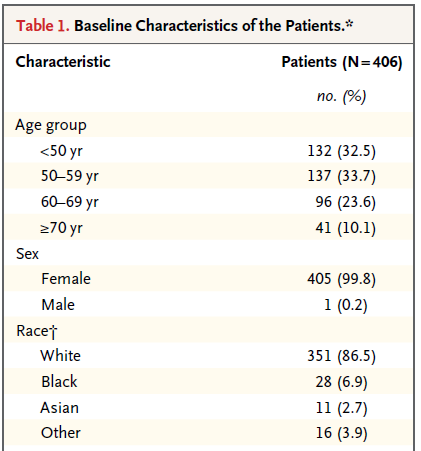
\includegraphics[width=0.5\linewidth]{images/Tolaney-snip1}

This (partial) table reports baseline characteristics on age group, sex
and race, describing 406 patients with HER2-positive\footnote{HER2 =
  human epidermal growth factor receptor type 2. Over-expression of this
  occurs in 15-20\% of invasive breast cancers, and has been associated
  with poor outcomes.} invasive breast cancer that began the protocol
therapy. Age, sex and race (along with severity of illness) are the most
commonly identified characteristics in a Table 1.

In addition to the measures shown in this excerpt, the full Table also
includes detailed information on the primary tumor for each patient,
including its size, nodal status and histologic grade. Footnotes tell us
that the percentages shown are subject to rounding, and may not total
100, and that the race information was self-reported.

\subsection{A group comparison}\label{a-group-comparison}

A more typical Table 1 involves a group comparison, for example in this
excerpt from \citet{Roy2008}. This Table 1 describes a multi-center
randomized clinical trial comparing two different approaches to caring
for patients with heart failure and atrial fibrillation\footnote{The
  complete Table 1 appears on pages 2668-2669 of \citet{Roy2008}, but I
  have only reproduced the first page and the footnote in this excerpt.}.

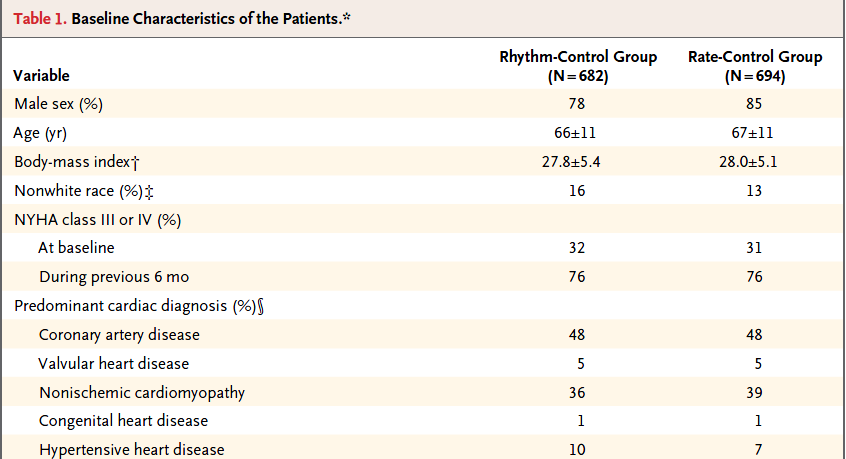
\includegraphics[width=0.9\linewidth]{images/Roy-snip1}

The article provides percentages, means and standard deviations across
groups, but note that it does not provide p values for the comparison of
baseline characteristics. This is a common feature of NEJM reports on
randomized clinical trials, where we anticipate that the two groups will
be well matched at baseline. Note that the patients in this study were
\emph{randomly} assigned to either the rhythm-control group or to the
rate-control group, using blocked randomizations stratified by study
center.

\section{The MR CLEAN trial}\label{the-mr-clean-trial}

\citet{Berkhemer2015} reported on the MR CLEAN trial, involving 500
patients with acute ischemic stroke caused by a proximal intracranial
arterial occlusion. The trial was conducted at 16 medical centers in the
Netherlands, where 233 were randomly assigned to the intervention
(intraarterial treatment plus usual care) and 267 to control (usual care
alone.) The primary outcome was the modified Rankin scale score at 90
days; this categorical scale measures functional outcome, with scores
ranging from 0 (no symptoms) to 6 (death). The fundamental conclusion of
\citet{Berkhemer2015} was that in patients with acute ischemic stroke
caused by a proximal intracranial occlusion of the anterior circulation,
intraarterial treatment administered within 6 hours after stroke onset
was effective and safe.

Here's the Table 1 from \citet{Berkhemer2015}.

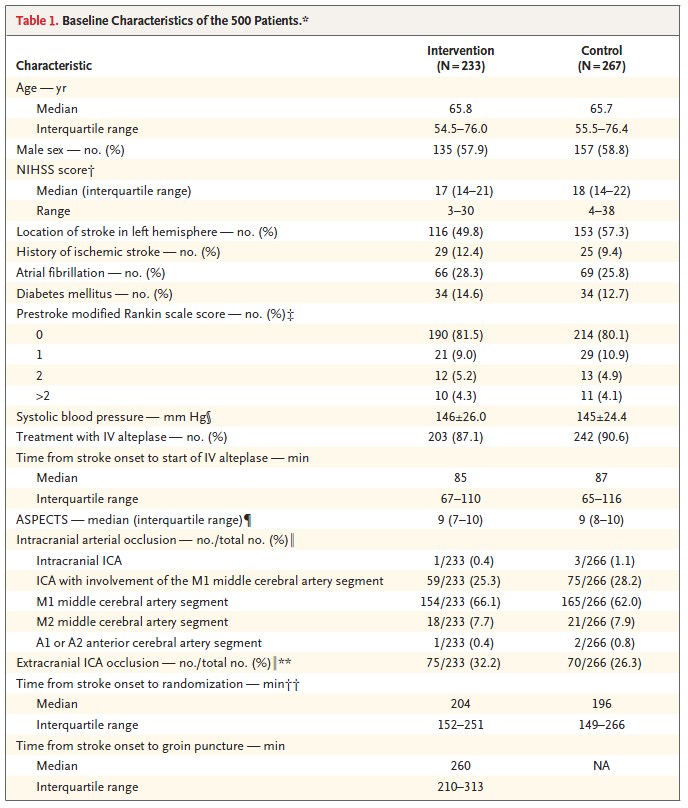
\includegraphics[width=0.9\linewidth]{images/Berkhemer-snip4complete}

The Table was accompanied by the following notes.

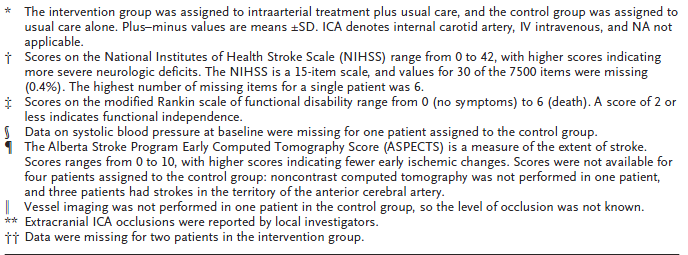
\includegraphics[width=0.9\linewidth]{images/Berkhemer-snip4notes}

\section{\texorpdfstring{Simulated \texttt{fakestroke}
data}{Simulated fakestroke data}}\label{simulated-fakestroke-data}

Consider the simulated data, available on the Data and Code page of
\href{https://github.com/THOMASELOVE/432-2018}{our course website} in
the \texttt{fakestroke.csv} file, which I built to let us mirror the
Table 1 for MR CLEAN \citep{Berkhemer2015}. The \texttt{fakestroke.csv}
file contains the following 18 variables for 500 patients.

\begin{longtable}[]{@{}rl@{}}
\toprule
\begin{minipage}[b]{0.16\columnwidth}\raggedleft\strut
Variable\strut
\end{minipage} & \begin{minipage}[b]{0.55\columnwidth}\raggedright\strut
Description\strut
\end{minipage}\tabularnewline
\midrule
\endhead
\begin{minipage}[t]{0.16\columnwidth}\raggedleft\strut
\texttt{studyid}\strut
\end{minipage} & \begin{minipage}[t]{0.55\columnwidth}\raggedright\strut
Study ID \# (z001 through z500)\strut
\end{minipage}\tabularnewline
\begin{minipage}[t]{0.16\columnwidth}\raggedleft\strut
\texttt{trt}\strut
\end{minipage} & \begin{minipage}[t]{0.55\columnwidth}\raggedright\strut
Treatment group (Intervention or Control)\strut
\end{minipage}\tabularnewline
\begin{minipage}[t]{0.16\columnwidth}\raggedleft\strut
\texttt{age}\strut
\end{minipage} & \begin{minipage}[t]{0.55\columnwidth}\raggedright\strut
Age in years\strut
\end{minipage}\tabularnewline
\begin{minipage}[t]{0.16\columnwidth}\raggedleft\strut
\texttt{sex}\strut
\end{minipage} & \begin{minipage}[t]{0.55\columnwidth}\raggedright\strut
Male or Female\strut
\end{minipage}\tabularnewline
\begin{minipage}[t]{0.16\columnwidth}\raggedleft\strut
\texttt{nihss}\strut
\end{minipage} & \begin{minipage}[t]{0.55\columnwidth}\raggedright\strut
NIH Stroke Scale Score (can range from 0-42; higher scores indicate more
severe neurological deficits)\strut
\end{minipage}\tabularnewline
\begin{minipage}[t]{0.16\columnwidth}\raggedleft\strut
\texttt{location}\strut
\end{minipage} & \begin{minipage}[t]{0.55\columnwidth}\raggedright\strut
Stroke Location - Left or Right Hemisphere\strut
\end{minipage}\tabularnewline
\begin{minipage}[t]{0.16\columnwidth}\raggedleft\strut
\texttt{hx.isch}\strut
\end{minipage} & \begin{minipage}[t]{0.55\columnwidth}\raggedright\strut
History of Ischemic Stroke (Yes/No)\strut
\end{minipage}\tabularnewline
\begin{minipage}[t]{0.16\columnwidth}\raggedleft\strut
\texttt{afib}\strut
\end{minipage} & \begin{minipage}[t]{0.55\columnwidth}\raggedright\strut
Atrial Fibrillation (1 = Yes, 0 = No)\strut
\end{minipage}\tabularnewline
\begin{minipage}[t]{0.16\columnwidth}\raggedleft\strut
\texttt{dm}\strut
\end{minipage} & \begin{minipage}[t]{0.55\columnwidth}\raggedright\strut
Diabetes Mellitus (1 = Yes, 0 = No)\strut
\end{minipage}\tabularnewline
\begin{minipage}[t]{0.16\columnwidth}\raggedleft\strut
\texttt{mrankin}\strut
\end{minipage} & \begin{minipage}[t]{0.55\columnwidth}\raggedright\strut
Pre-stroke modified Rankin scale score (0, 1, 2 or \textgreater{} 2)
indicating functional disability - complete range is 0 (no symptoms) to
6 (death)\strut
\end{minipage}\tabularnewline
\begin{minipage}[t]{0.16\columnwidth}\raggedleft\strut
\texttt{sbp}\strut
\end{minipage} & \begin{minipage}[t]{0.55\columnwidth}\raggedright\strut
Systolic blood pressure, in mm Hg\strut
\end{minipage}\tabularnewline
\begin{minipage}[t]{0.16\columnwidth}\raggedleft\strut
\texttt{iv.altep}\strut
\end{minipage} & \begin{minipage}[t]{0.55\columnwidth}\raggedright\strut
Treatment with IV alteplase (Yes/No)\strut
\end{minipage}\tabularnewline
\begin{minipage}[t]{0.16\columnwidth}\raggedleft\strut
\texttt{time.iv}\strut
\end{minipage} & \begin{minipage}[t]{0.55\columnwidth}\raggedright\strut
Time from stroke onset to start of IV alteplase (minutes) if
iv.altep=Yes\strut
\end{minipage}\tabularnewline
\begin{minipage}[t]{0.16\columnwidth}\raggedleft\strut
\texttt{aspects}\strut
\end{minipage} & \begin{minipage}[t]{0.55\columnwidth}\raggedright\strut
Alberta Stroke Program Early Computed Tomography score, which measures
extent of stroke from 0 - 10; higher scores indicate fewer early
ischemic changes\strut
\end{minipage}\tabularnewline
\begin{minipage}[t]{0.16\columnwidth}\raggedleft\strut
\texttt{ia.occlus}\strut
\end{minipage} & \begin{minipage}[t]{0.55\columnwidth}\raggedright\strut
Intracranial arterial occlusion, based on vessel imaging - five
categories\footnotemark{}\strut
\end{minipage}
\footnotetext{The five categories are Intracranial ICA, ICA with
  involvement of the M1 middle cerebral artery segment, M1 middle
  cerebral artery segment, M2 middle cerebral artery segment, A1 or A2
  anterior cerebral artery segment}\tabularnewline
\begin{minipage}[t]{0.16\columnwidth}\raggedleft\strut
\texttt{extra.ica}\strut
\end{minipage} & \begin{minipage}[t]{0.55\columnwidth}\raggedright\strut
Extracranial ICA occlusion (1 = Yes, 0 = No)\strut
\end{minipage}\tabularnewline
\begin{minipage}[t]{0.16\columnwidth}\raggedleft\strut
\texttt{time.rand}\strut
\end{minipage} & \begin{minipage}[t]{0.55\columnwidth}\raggedright\strut
Time from stroke onset to study randomization, in minutes\strut
\end{minipage}\tabularnewline
\begin{minipage}[t]{0.16\columnwidth}\raggedleft\strut
\texttt{time.punc}\strut
\end{minipage} & \begin{minipage}[t]{0.55\columnwidth}\raggedright\strut
Time from stroke onset to groin puncture, in minutes (only if
Intervention)\strut
\end{minipage}\tabularnewline
\bottomrule
\end{longtable}

Here's a quick look at the simulated data in \texttt{fakestroke}.

\begin{Shaded}
\begin{Highlighting}[]
\NormalTok{fakestroke}
\end{Highlighting}
\end{Shaded}

\begin{verbatim}
# A tibble: 500 x 18
   studyid trt        age sex   nihss location hx.isch  afib    dm mrankin
   <fct>   <fct>    <dbl> <fct> <int> <fct>    <fct>   <int> <int> <fct>  
 1 z001    Control   53.0 Male     21 Right    No          0     0 2      
 2 z002    Interve~  51.0 Male     23 Left     No          1     0 0      
 3 z003    Control   68.0 Fema~    11 Right    No          0     0 0      
 4 z004    Control   28.0 Male     22 Left     No          0     0 0      
 5 z005    Control   91.0 Male     24 Right    No          0     0 0      
 6 z006    Control   34.0 Fema~    18 Left     No          0     0 2      
 7 z007    Interve~  75.0 Male     25 Right    No          0     0 0      
 8 z008    Control   89.0 Fema~    18 Right    No          0     0 0      
 9 z009    Control   75.0 Male     25 Left     No          1     0 2      
10 z010    Interve~  26.0 Fema~    27 Right    No          0     0 0      
# ... with 490 more rows, and 8 more variables: sbp <int>, iv.altep <fct>,
#   time.iv <int>, aspects <int>, ia.occlus <fct>, extra.ica <int>,
#   time.rand <int>, time.punc <int>
\end{verbatim}

\section{\texorpdfstring{Building Table 1 for \texttt{fakestroke}:
Attempt
1}{Building Table 1 for fakestroke: Attempt 1}}\label{building-table-1-for-fakestroke-attempt-1}

Our goal, then, is to take the data in \texttt{fakestroke.csv} and use
it to generate a Table 1 for the study that compares the 233 patients in
the Intervention group to the 267 patients in the Control group, on all
of the other variables (except study ID \#) available. I'll use the
\texttt{tableone} package of functions available in R to help me
complete this task. We'll make a first attempt, using the
\texttt{CreateTableOne} function in the \texttt{tableone} package. To
use the function, we'll need to specify:

\begin{itemize}
\tightlist
\item
  the \texttt{vars} or variables we want to place in the rows of our
  Table 1 (which will include just about everything in the
  \texttt{fakestroke} data except the \texttt{studyid} code and the
  \texttt{trt} variable for which we have other plans, and the
  \texttt{time.punc} which applies only to subjects in the Intervention
  group.)

  \begin{itemize}
  \tightlist
  \item
    A useful trick here is to use the \texttt{dput} function,
    specifically something like \texttt{dput(names(fakestroke))} can be
    used to generate a list of all of the variables included in the
    \texttt{fakestroke} tibble, and then this can be copied and pasted
    into the \texttt{vars} specification, saving some typing.
  \end{itemize}
\item
  the \texttt{strata} which indicates the levels want to use in the
  columns of our Table 1 (for us, that's \texttt{trt})
\end{itemize}

\begin{Shaded}
\begin{Highlighting}[]
\NormalTok{fs.vars <-}\StringTok{ }\KeywordTok{c}\NormalTok{(}\StringTok{"age"}\NormalTok{, }\StringTok{"sex"}\NormalTok{, }\StringTok{"nihss"}\NormalTok{, }\StringTok{"location"}\NormalTok{, }
          \StringTok{"hx.isch"}\NormalTok{, }\StringTok{"afib"}\NormalTok{, }\StringTok{"dm"}\NormalTok{, }\StringTok{"mrankin"}\NormalTok{, }\StringTok{"sbp"}\NormalTok{,}
          \StringTok{"iv.altep"}\NormalTok{, }\StringTok{"time.iv"}\NormalTok{, }\StringTok{"aspects"}\NormalTok{, }
          \StringTok{"ia.occlus"}\NormalTok{, }\StringTok{"extra.ica"}\NormalTok{, }\StringTok{"time.rand"}\NormalTok{)}

\NormalTok{fs.trt <-}\StringTok{ }\KeywordTok{c}\NormalTok{(}\StringTok{"trt"}\NormalTok{)}

\NormalTok{att1 <-}\StringTok{ }\KeywordTok{CreateTableOne}\NormalTok{(}\DataTypeTok{data =}\NormalTok{ fakestroke, }
                       \DataTypeTok{vars =}\NormalTok{ fs.vars, }
                       \DataTypeTok{strata =}\NormalTok{ fs.trt)}
\KeywordTok{print}\NormalTok{(att1)}
\end{Highlighting}
\end{Shaded}

\begin{verbatim}
                       Stratified by trt
                        Control        Intervention   p      test
  n                        267            233                    
  age (mean (sd))        65.38 (16.10)  63.93 (18.09)  0.343     
  sex = Male (%)           157 (58.8)     135 (57.9)   0.917     
  nihss (mean (sd))      18.08 (4.32)   17.97 (5.04)   0.787     
  location = Right (%)     114 (42.7)     117 (50.2)   0.111     
  hx.isch = Yes (%)         25 ( 9.4)      29 (12.4)   0.335     
  afib (mean (sd))        0.26 (0.44)    0.28 (0.45)   0.534     
  dm (mean (sd))          0.13 (0.33)    0.12 (0.33)   0.923     
  mrankin (%)                                          0.922     
     > 2                    11 ( 4.1)      10 ( 4.3)             
     0                     214 (80.1)     190 (81.5)             
     1                      29 (10.9)      21 ( 9.0)             
     2                      13 ( 4.9)      12 ( 5.2)             
  sbp (mean (sd))       145.00 (24.40) 146.03 (26.00)  0.647     
  iv.altep = Yes (%)       242 (90.6)     203 (87.1)   0.267     
  time.iv (mean (sd))    87.96 (26.01)  98.22 (45.48)  0.003     
  aspects (mean (sd))     8.65 (1.47)    8.35 (1.64)   0.033     
  ia.occlus (%)                                        0.795     
     A1 or A2                2 ( 0.8)       1 ( 0.4)             
     ICA with M1            75 (28.2)      59 (25.3)             
     Intracranial ICA        3 ( 1.1)       1 ( 0.4)             
     M1                    165 (62.0)     154 (66.1)             
     M2                     21 ( 7.9)      18 ( 7.7)             
  extra.ica (mean (sd))   0.26 (0.44)    0.32 (0.47)   0.150     
  time.rand (mean (sd)) 213.88 (70.29) 202.51 (57.33)  0.051     
\end{verbatim}

\subsection{Some of this is very useful, and other parts need to be
fixed.}\label{some-of-this-is-very-useful-and-other-parts-need-to-be-fixed.}

\begin{enumerate}
\def\labelenumi{\arabic{enumi}.}
\tightlist
\item
  The 1/0 variables (\texttt{afib}, \texttt{dm}, \texttt{extra.ica})
  might be better if they were treated as the factors they are, and
  reported as the Yes/No variables are reported, with counts and
  percentages rather than with means and standard deviations.
\item
  In some cases, we may prefer to re-order the levels of the categorical
  (factor) variables, particularly the \texttt{mrankin} variable, but
  also the \texttt{ia.occlus} variable. It would also be more typical to
  put the Intervention group to the left and the Control group to the
  right, so we may need to adjust our \texttt{trt} variable's levels
  accordingly.
\item
  For each of the quantitative variables (\texttt{age}, \texttt{nihss},
  \texttt{sbp}, \texttt{time.iv}, \texttt{aspects}, \texttt{extra.ica},
  \texttt{time.rand} and \texttt{time.punc}) we should make a decision
  whether a summary with mean and standard deviation is appropriate, or
  whether we should instead summarize with, say, the median and
  quartiles. A mean and standard deviation really only yields an
  appropriate summary when the data are least approximately Normally
  distributed. This will make the \emph{p} values a bit more reasonable,
  too. The \texttt{test} column in the first attempt will soon have
  something useful to tell us.
\item
  If we'd left in the \texttt{time.punc} variable, we'd get some
  warnings, having to do with the fact that \texttt{time.punc} is only
  relevant to patients in the Intervention group.
\end{enumerate}

\subsection{\texorpdfstring{\texttt{fakestroke} Cleaning Up Categorical
Variables}{fakestroke Cleaning Up Categorical Variables}}\label{fakestroke-cleaning-up-categorical-variables}

Let's specify each of the categorical variables as categorical
explicitly. This helps the \texttt{CreateTableOne} function treat them
appropriately, and display them with counts and percentages. This
includes all of the 1/0, Yes/No and multi-categorical variables.

\begin{Shaded}
\begin{Highlighting}[]
\NormalTok{fs.factorvars <-}\StringTok{ }\KeywordTok{c}\NormalTok{(}\StringTok{"sex"}\NormalTok{, }\StringTok{"location"}\NormalTok{, }\StringTok{"hx.isch"}\NormalTok{, }\StringTok{"afib"}\NormalTok{, }\StringTok{"dm"}\NormalTok{, }
                   \StringTok{"mrankin"}\NormalTok{, }\StringTok{"iv.altep"}\NormalTok{, }\StringTok{"ia.occlus"}\NormalTok{, }\StringTok{"extra.ica"}\NormalTok{)}
\end{Highlighting}
\end{Shaded}

Then we simply add a \texttt{factorVars\ =\ fs.factorvars} call to the
\texttt{CreateTableOne} function.

We also want to re-order some of those categorical variables, so that
the levels are more useful to us. Specifically, we want to:

\begin{itemize}
\tightlist
\item
  place Intervention before Control in the \texttt{trt} variable,
\item
  reorder the \texttt{mrankin} scale as 0, 1, 2, \textgreater{} 2, and
\item
  rearrange the \texttt{ia.occlus} variable to the order\footnote{We
    might also have considered reordering the \texttt{ia.occlus} factor
    by its frequency, using the \texttt{fct\_infreq} function} presented
  in \citet{Berkhemer2015}.
\end{itemize}

To accomplish this, we'll use the \texttt{fct\_relevel} function from
the \texttt{forcats} package (loaded with the rest of the core
\texttt{tidyverse} packages) to reorder our levels manually.

\begin{Shaded}
\begin{Highlighting}[]
\NormalTok{fakestroke <-}\StringTok{ }\NormalTok{fakestroke }\OperatorTok
\StringTok{    }\KeywordTok{mutate}\NormalTok{(}\DataTypeTok{trt =} \KeywordTok{fct_relevel}\NormalTok{(trt, }\StringTok{"Intervention"}\NormalTok{, }\StringTok{"Control"}\NormalTok{),}
           \DataTypeTok{mrankin =} \KeywordTok{fct_relevel}\NormalTok{(mrankin, }\StringTok{"0"}\NormalTok{, }\StringTok{"1"}\NormalTok{, }\StringTok{"2"}\NormalTok{, }\StringTok{"> 2"}\NormalTok{),}
           \DataTypeTok{ia.occlus =} \KeywordTok{fct_relevel}\NormalTok{(ia.occlus, }\StringTok{"Intracranial ICA"}\NormalTok{, }
                                   \StringTok{"ICA with M1"}\NormalTok{, }\StringTok{"M1"}\NormalTok{, }\StringTok{"M2"}\NormalTok{, }
                                   \StringTok{"A1 or A2"}\NormalTok{)}
\NormalTok{           ) }
\end{Highlighting}
\end{Shaded}

\section{\texorpdfstring{\texttt{fakestroke} Table 1: Attempt
2}{fakestroke Table 1: Attempt 2}}\label{fakestroke-table-1-attempt-2}

\begin{Shaded}
\begin{Highlighting}[]
\NormalTok{att2 <-}\StringTok{ }\KeywordTok{CreateTableOne}\NormalTok{(}\DataTypeTok{data =}\NormalTok{ fakestroke, }
                       \DataTypeTok{vars =}\NormalTok{ fs.vars,}
                       \DataTypeTok{factorVars =}\NormalTok{ fs.factorvars,}
                       \DataTypeTok{strata =}\NormalTok{ fs.trt)}
\KeywordTok{print}\NormalTok{(att2)}
\end{Highlighting}
\end{Shaded}

\begin{verbatim}
                       Stratified by trt
                        Intervention   Control        p      test
  n                        233            267                    
  age (mean (sd))        63.93 (18.09)  65.38 (16.10)  0.343     
  sex = Male (%)           135 (57.9)     157 (58.8)   0.917     
  nihss (mean (sd))      17.97 (5.04)   18.08 (4.32)   0.787     
  location = Right (%)     117 (50.2)     114 (42.7)   0.111     
  hx.isch = Yes (%)         29 (12.4)      25 ( 9.4)   0.335     
  afib = 1 (%)              66 (28.3)      69 (25.8)   0.601     
  dm = 1 (%)                29 (12.4)      34 (12.7)   1.000     
  mrankin (%)                                          0.922     
     0                     190 (81.5)     214 (80.1)             
     1                      21 ( 9.0)      29 (10.9)             
     2                      12 ( 5.2)      13 ( 4.9)             
     > 2                    10 ( 4.3)      11 ( 4.1)             
  sbp (mean (sd))       146.03 (26.00) 145.00 (24.40)  0.647     
  iv.altep = Yes (%)       203 (87.1)     242 (90.6)   0.267     
  time.iv (mean (sd))    98.22 (45.48)  87.96 (26.01)  0.003     
  aspects (mean (sd))     8.35 (1.64)    8.65 (1.47)   0.033     
  ia.occlus (%)                                        0.795     
     Intracranial ICA        1 ( 0.4)       3 ( 1.1)             
     ICA with M1            59 (25.3)      75 (28.2)             
     M1                    154 (66.1)     165 (62.0)             
     M2                     18 ( 7.7)      21 ( 7.9)             
     A1 or A2                1 ( 0.4)       2 ( 0.8)             
  extra.ica = 1 (%)         75 (32.2)      70 (26.3)   0.179     
  time.rand (mean (sd)) 202.51 (57.33) 213.88 (70.29)  0.051     
\end{verbatim}

The categorical data presentation looks much improved.

\subsection{What summaries should we
show?}\label{what-summaries-should-we-show}

Now, we'll move on to the issue of making a decision about what type of
summary to show for the quantitative variables. Since the
\texttt{fakestroke} data are just simulated and only match the summary
statistics of the original results, not the details, we'll adopt the
decisions made by \citet{Berkhemer2015}, which were to use medians and
interquartile ranges to summarize the distributions of all of the
continuous variables \textbf{except} systolic blood pressure.

\begin{itemize}
\tightlist
\item
  Specifying certain quantitative variables as \emph{non-normal} causes
  R to show them with medians and the 25th and 75th percentiles, rather
  than means and standard deviations, and also causes those variables to
  be tested using non-parametric tests, like the Wilcoxon signed rank
  test, rather than the t test. The \texttt{test} column indicates this
  with the word \texttt{nonnorm}.

  \begin{itemize}
  \tightlist
  \item
    In real data situations, what should we do? The answer is to look at
    the data. I would not make the decision as to which approach to take
    without first plotting (perhaps in a histogram or a Normal Q-Q plot)
    the observed distributions in each of the two samples, so that I
    could make a sound decision about whether Normality was a reasonable
    assumption. If the means and medians are meaningfully different from
    each other, this is especially important.
  \item
    To be honest, though, if the variable in question is a relatively
    unimportant covariate and the \emph{p} values for the two approaches
    are nearly the same, I'm not sure that further investigation is
    especially important,
  \end{itemize}
\item
  Specifying \emph{exact} tests for certain categorical variables (we'll
  try this for the \texttt{location} and \texttt{mrankin} variables) can
  be done, and these changes will be noted in the \texttt{test} column,
  as well.

  \begin{itemize}
  \tightlist
  \item
    In real data situations, I would rarely be concerned about this
    issue, and often choose Pearson (approximate) options across the
    board. This is reasonable so long as the number of subjects falling
    in each category is reasonably large, say above 10. If not, then an
    exact test may be an improvement.
  \end{itemize}
\end{itemize}

To accomplish the Table 1, then, we need to specify which variables
should be treated as non-Normal in the \texttt{print} statement - notice
that we don't need to redo the \texttt{CreateTableOne} for this change.

\begin{Shaded}
\begin{Highlighting}[]
\KeywordTok{print}\NormalTok{(att2, }
      \DataTypeTok{nonnormal =} \KeywordTok{c}\NormalTok{(}\StringTok{"age"}\NormalTok{, }\StringTok{"nihss"}\NormalTok{, }\StringTok{"time.iv"}\NormalTok{, }\StringTok{"aspects"}\NormalTok{, }\StringTok{"time.rand"}\NormalTok{),}
      \DataTypeTok{exact =} \KeywordTok{c}\NormalTok{(}\StringTok{"location"}\NormalTok{, }\StringTok{"mrankin"}\NormalTok{))}
\end{Highlighting}
\end{Shaded}

\begin{verbatim}
                          Stratified by trt
                           Intervention            Control                
  n                           233                     267                 
  age (median [IQR])        65.80 [54.50, 76.00]    65.70 [55.75, 76.20]  
  sex = Male (%)              135 (57.9)              157 (58.8)          
  nihss (median [IQR])      17.00 [14.00, 21.00]    18.00 [14.00, 22.00]  
  location = Right (%)        117 (50.2)              114 (42.7)          
  hx.isch = Yes (%)            29 (12.4)               25 ( 9.4)          
  afib = 1 (%)                 66 (28.3)               69 (25.8)          
  dm = 1 (%)                   29 (12.4)               34 (12.7)          
  mrankin (%)                                                             
     0                        190 (81.5)              214 (80.1)          
     1                         21 ( 9.0)               29 (10.9)          
     2                         12 ( 5.2)               13 ( 4.9)          
     > 2                       10 ( 4.3)               11 ( 4.1)          
  sbp (mean (sd))          146.03 (26.00)          145.00 (24.40)         
  iv.altep = Yes (%)          203 (87.1)              242 (90.6)          
  time.iv (median [IQR])    85.00 [67.00, 110.00]   87.00 [65.00, 116.00] 
  aspects (median [IQR])     9.00 [7.00, 10.00]      9.00 [8.00, 10.00]   
  ia.occlus (%)                                                           
     Intracranial ICA           1 ( 0.4)                3 ( 1.1)          
     ICA with M1               59 (25.3)               75 (28.2)          
     M1                       154 (66.1)              165 (62.0)          
     M2                        18 ( 7.7)               21 ( 7.9)          
     A1 or A2                   1 ( 0.4)                2 ( 0.8)          
  extra.ica = 1 (%)            75 (32.2)               70 (26.3)          
  time.rand (median [IQR]) 204.00 [152.00, 249.50] 196.00 [149.00, 266.00]
                          Stratified by trt
                           p      test   
  n                                      
  age (median [IQR])        0.579 nonnorm
  sex = Male (%)            0.917        
  nihss (median [IQR])      0.453 nonnorm
  location = Right (%)      0.106 exact  
  hx.isch = Yes (%)         0.335        
  afib = 1 (%)              0.601        
  dm = 1 (%)                1.000        
  mrankin (%)               0.917 exact  
     0                                   
     1                                   
     2                                   
     > 2                                 
  sbp (mean (sd))           0.647        
  iv.altep = Yes (%)        0.267        
  time.iv (median [IQR])    0.596 nonnorm
  aspects (median [IQR])    0.075 nonnorm
  ia.occlus (%)             0.795        
     Intracranial ICA                    
     ICA with M1                         
     M1                                  
     M2                                  
     A1 or A2                            
  extra.ica = 1 (%)         0.179        
  time.rand (median [IQR])  0.251 nonnorm
\end{verbatim}

\section{Obtaining a more detailed
Summary}\label{obtaining-a-more-detailed-summary}

If this was a real data set, we'd want to get a more detailed
description of the data to make decisions about things like potentially
collapsing categories of a variable, or whether or not a normal
distribution was useful for a particular continuous variable, etc. You
can do this with the \texttt{summary} command applied to a created Table
1, which shows, among other things, the effect of changing from normal
to non-normal \emph{p} values for continuous variables, and from
approximate to ``exact'' \emph{p} values for categorical factors.

Again, as noted above, in a real data situation, we'd want to plot the
quantitative variables (within each group) to make a smart decision
about whether a t test or Wilcoxon approach is more appropriate.

Note in the summary below that we have some missing values here. Often,
we'll present this information within the Table 1, as well.

\begin{Shaded}
\begin{Highlighting}[]
\KeywordTok{summary}\NormalTok{(att2)}
\end{Highlighting}
\end{Shaded}

\begin{verbatim}

     ### Summary of continuous variables ###

trt: Intervention
            n miss p.miss mean sd median p25 p75 min max  skew  kurt
age       233    0    0.0   64 18     66  54  76  23  96 -0.34 -0.52
nihss     233    0    0.0   18  5     17  14  21  10  28  0.48 -0.74
sbp       233    0    0.0  146 26    146 129 164  78 214 -0.07 -0.22
time.iv   233   30   12.9   98 45     85  67 110  42 218  1.03  0.08
aspects   233    0    0.0    8  2      9   7  10   5  10 -0.56 -0.98
time.rand 233    2    0.9  203 57    204 152 250 100 300  0.01 -1.16
-------------------------------------------------------- 
trt: Control
            n miss p.miss mean sd median p25 p75 min max   skew  kurt
age       267    0    0.0   65 16     66  56  76  24  94 -0.296 -0.28
nihss     267    0    0.0   18  4     18  14  22  11  25  0.017 -1.24
sbp       267    1    0.4  145 24    145 128 161  82 231  0.156  0.08
time.iv   267   25    9.4   88 26     87  65 116  44 130  0.001 -1.32
aspects   267    4    1.5    9  1      9   8  10   5  10 -1.071  0.36
time.rand 267    0    0.0  214 70    196 149 266 120 360  0.508 -0.93

p-values
              pNormal pNonNormal
age       0.342813660 0.57856976
nihss     0.787487252 0.45311695
sbp       0.647157646 0.51346132
time.iv   0.003073372 0.59641104
aspects   0.032662901 0.07464683
time.rand 0.050803672 0.25134327

Standardize mean differences
              1 vs 2
age       0.08478764
nihss     0.02405390
sbp       0.04100833
time.iv   0.27691223
aspects   0.19210662
time.rand 0.17720957

=======================================================================================

     ### Summary of categorical variables ### 

trt: Intervention
       var   n miss p.miss            level freq percent cum.percent
       sex 233    0    0.0           Female   98    42.1        42.1
                                       Male  135    57.9       100.0
                                                                    
  location 233    0    0.0             Left  116    49.8        49.8
                                      Right  117    50.2       100.0
                                                                    
   hx.isch 233    0    0.0               No  204    87.6        87.6
                                        Yes   29    12.4       100.0
                                                                    
      afib 233    0    0.0                0  167    71.7        71.7
                                          1   66    28.3       100.0
                                                                    
        dm 233    0    0.0                0  204    87.6        87.6
                                          1   29    12.4       100.0
                                                                    
   mrankin 233    0    0.0                0  190    81.5        81.5
                                          1   21     9.0        90.6
                                          2   12     5.2        95.7
                                        > 2   10     4.3       100.0
                                                                    
  iv.altep 233    0    0.0               No   30    12.9        12.9
                                        Yes  203    87.1       100.0
                                                                    
 ia.occlus 233    0    0.0 Intracranial ICA    1     0.4         0.4
                                ICA with M1   59    25.3        25.8
                                         M1  154    66.1        91.8
                                         M2   18     7.7        99.6
                                   A1 or A2    1     0.4       100.0
                                                                    
 extra.ica 233    0    0.0                0  158    67.8        67.8
                                          1   75    32.2       100.0
                                                                    
-------------------------------------------------------- 
trt: Control
       var   n miss p.miss            level freq percent cum.percent
       sex 267    0    0.0           Female  110    41.2        41.2
                                       Male  157    58.8       100.0
                                                                    
  location 267    0    0.0             Left  153    57.3        57.3
                                      Right  114    42.7       100.0
                                                                    
   hx.isch 267    0    0.0               No  242    90.6        90.6
                                        Yes   25     9.4       100.0
                                                                    
      afib 267    0    0.0                0  198    74.2        74.2
                                          1   69    25.8       100.0
                                                                    
        dm 267    0    0.0                0  233    87.3        87.3
                                          1   34    12.7       100.0
                                                                    
   mrankin 267    0    0.0                0  214    80.1        80.1
                                          1   29    10.9        91.0
                                          2   13     4.9        95.9
                                        > 2   11     4.1       100.0
                                                                    
  iv.altep 267    0    0.0               No   25     9.4         9.4
                                        Yes  242    90.6       100.0
                                                                    
 ia.occlus 267    1    0.4 Intracranial ICA    3     1.1         1.1
                                ICA with M1   75    28.2        29.3
                                         M1  165    62.0        91.4
                                         M2   21     7.9        99.2
                                   A1 or A2    2     0.8       100.0
                                                                    
 extra.ica 267    1    0.4                0  196    73.7        73.7
                                          1   70    26.3       100.0
                                                                    

p-values
            pApprox    pExact
sex       0.9171387 0.8561188
location  0.1113553 0.1056020
hx.isch   0.3352617 0.3124683
afib      0.6009691 0.5460206
dm        1.0000000 1.0000000
mrankin   0.9224798 0.9173657
iv.altep  0.2674968 0.2518374
ia.occlus 0.7945580 0.8189090
extra.ica 0.1793385 0.1667574

Standardize mean differences
               1 vs 2
sex       0.017479025
location  0.151168444
hx.isch   0.099032275
afib      0.055906317
dm        0.008673478
mrankin   0.062543164
iv.altep  0.111897009
ia.occlus 0.117394890
extra.ica 0.129370206
\end{verbatim}

In this case, I have simulated the data to mirror the results in the
published Table 1 for this study. In no way have I captured the full
range of the real data, or any of the relationships in that data, so
it's more important here to see what's available in the analysis, rather
than to interpret it closely in the clinical context.

\section{Exporting the Completed Table 1 from R to Excel or
Word}\label{exporting-the-completed-table-1-from-r-to-excel-or-word}

Once you've built the table and are generally satisfied with it, you'll
probably want to be able to drop it into Excel or Word for final
cleanup.

\subsection{Approach A: Save and open in
Excel}\label{approach-a-save-and-open-in-excel}

One option is to \textbf{save the Table 1} to a \texttt{.csv} file,
which you can then open directly in Excel. This is the approach I
generally use. Note the addition of some \texttt{quote},
\texttt{noSpaces} and \texttt{printToggle} selections here.

\begin{Shaded}
\begin{Highlighting}[]
\NormalTok{fs.table1save <-}\StringTok{ }\KeywordTok{print}\NormalTok{(att2, }
      \DataTypeTok{nonnormal =} \KeywordTok{c}\NormalTok{(}\StringTok{"age"}\NormalTok{, }\StringTok{"nihss"}\NormalTok{, }\StringTok{"time.iv"}\NormalTok{, }\StringTok{"aspects"}\NormalTok{, }\StringTok{"time.rand"}\NormalTok{),}
      \DataTypeTok{exact =} \KeywordTok{c}\NormalTok{(}\StringTok{"location"}\NormalTok{, }\StringTok{"mrankin"}\NormalTok{),}
      \DataTypeTok{quote =} \OtherTok{FALSE}\NormalTok{, }\DataTypeTok{noSpaces =} \OtherTok{TRUE}\NormalTok{, }\DataTypeTok{printToggle =} \OtherTok{FALSE}\NormalTok{)}

\KeywordTok{write.csv}\NormalTok{(fs.table1save, }\DataTypeTok{file =} \StringTok{"fs-table1.csv"}\NormalTok{)}
\end{Highlighting}
\end{Shaded}

When I then open the \texttt{fs-table1.csv} file in Excel, it looks like
this:

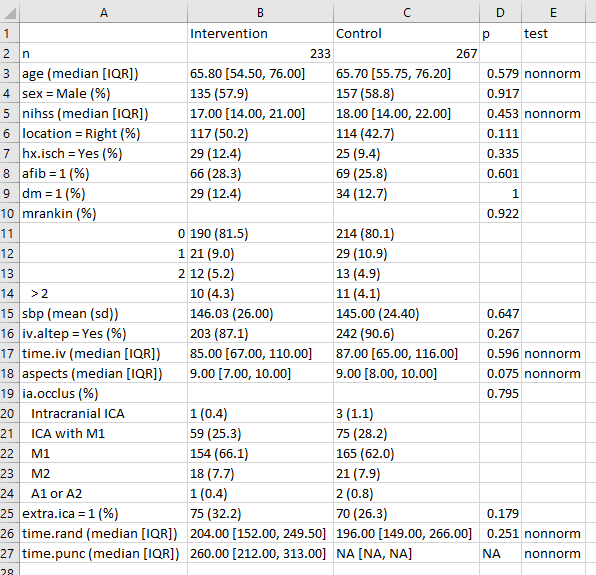
\includegraphics[width=0.9\linewidth]{images/fs-table1inExcel}

And from here, I can either drop it directly into Word, or present it as
is, or start tweaking it to meet formatting needs.

\subsection{Approach B: Produce the Table so you can cut and paste
it}\label{approach-b-produce-the-table-so-you-can-cut-and-paste-it}

\begin{Shaded}
\begin{Highlighting}[]
\KeywordTok{print}\NormalTok{(att2, }
      \DataTypeTok{nonnormal =} \KeywordTok{c}\NormalTok{(}\StringTok{"age"}\NormalTok{, }\StringTok{"nihss"}\NormalTok{, }\StringTok{"time.iv"}\NormalTok{, }\StringTok{"aspects"}\NormalTok{, }\StringTok{"time.rand"}\NormalTok{),}
      \DataTypeTok{exact =} \KeywordTok{c}\NormalTok{(}\StringTok{"location"}\NormalTok{, }\StringTok{"mrankin"}\NormalTok{),}
      \DataTypeTok{quote =} \OtherTok{TRUE}\NormalTok{, }\DataTypeTok{noSpaces =} \OtherTok{TRUE}\NormalTok{)}
\end{Highlighting}
\end{Shaded}

This will look like a mess by itself, but if you:

\begin{enumerate}
\def\labelenumi{\arabic{enumi}.}
\tightlist
\item
  copy and paste that mess into Excel
\item
  select Text to Columns from the Data menu
\item
  select Delimited, then Space and select Treat consecutive delimiters
  as one
\end{enumerate}

you should get something usable again.

Or, in Word,

\begin{enumerate}
\def\labelenumi{\arabic{enumi}.}
\tightlist
\item
  insert the text
\item
  select the text with your mouse
\item
  select Insert \ldots{} Table \ldots{} Convert Text to Table
\item
  place a quotation mark in the ``Other'' area under Separate text at
  \ldots{}
\end{enumerate}

After dropping blank columns, the result looks pretty good.

\section{A Controlled Biological Experiment - The Blood-Brain
Barrier}\label{a-controlled-biological-experiment---the-blood-brain-barrier}

My source for the data and the following explanatory paragraph is page
307 from \citet{RamseySchafer2002}. The original data come from
\citet{Barnett1995}.

\begin{quote}
The human brain (and that of rats, coincidentally) is protected from the
bacteria and toxins that course through the bloodstream by something
called the blood-brain barrier. After a method of disrupting the barrier
was developed, researchers tested this new mechanism, as follows. A
series of 34 rats were inoculated with human lung cancer cells to induce
brain tumors. After 9-11 days they were infused with either the barrier
disruption (BD) solution or, as a control, a normal saline (NS)
solution. Fifteen minutes later, the rats received a standard dose of a
particular therapeutic antibody (L6-F(ab')2. The key measure of the
effectiveness of transmission across the brain-blood barrier is the
ratio of the antibody concentration in the brain tumor to the antibody
concentration in normal tissue outside the brain. The rats were then
sacrificed, and the amounts of antibody in the brain tumor and in normal
tissue from the liver were measured. The study's primary objective is to
determine whether the antibody concentration in the tumor increased when
the blood-barrier disruption infusion was given, and if so, by how much?
\end{quote}

\section{\texorpdfstring{The \texttt{bloodbrain.csv}
file}{The bloodbrain.csv file}}\label{the-bloodbrain.csv-file}

Consider the data, available on the Data and Code page of
\href{https://github.com/THOMASELOVE/432-2018}{our course website} in
the \texttt{bloodbrain.csv} file, which includes the following
variables:

\begin{longtable}[]{@{}rl@{}}
\toprule
\begin{minipage}[b]{0.12\columnwidth}\raggedleft\strut
Variable\strut
\end{minipage} & \begin{minipage}[b]{0.59\columnwidth}\raggedright\strut
Description\strut
\end{minipage}\tabularnewline
\midrule
\endhead
\begin{minipage}[t]{0.12\columnwidth}\raggedleft\strut
\texttt{case}\strut
\end{minipage} & \begin{minipage}[t]{0.59\columnwidth}\raggedright\strut
identification number for the rat (1 - 34)\strut
\end{minipage}\tabularnewline
\begin{minipage}[t]{0.12\columnwidth}\raggedleft\strut
\texttt{brain}\strut
\end{minipage} & \begin{minipage}[t]{0.59\columnwidth}\raggedright\strut
an outcome: Brain tumor antibody count (per gram)\strut
\end{minipage}\tabularnewline
\begin{minipage}[t]{0.12\columnwidth}\raggedleft\strut
\texttt{liver}\strut
\end{minipage} & \begin{minipage}[t]{0.59\columnwidth}\raggedright\strut
an outcome: Liver antibody count (per gram)\strut
\end{minipage}\tabularnewline
\begin{minipage}[t]{0.12\columnwidth}\raggedleft\strut
\texttt{tlratio}\strut
\end{minipage} & \begin{minipage}[t]{0.59\columnwidth}\raggedright\strut
an outcome: tumor / liver concentration ratio\strut
\end{minipage}\tabularnewline
\begin{minipage}[t]{0.12\columnwidth}\raggedleft\strut
\texttt{solution}\strut
\end{minipage} & \begin{minipage}[t]{0.59\columnwidth}\raggedright\strut
the treatment: BD (barrier disruption) or NS (normal saline)\strut
\end{minipage}\tabularnewline
\begin{minipage}[t]{0.12\columnwidth}\raggedleft\strut
\texttt{sactime}\strut
\end{minipage} & \begin{minipage}[t]{0.59\columnwidth}\raggedright\strut
a design variable: Sacrifice time (hours; either 0.5, 3, 24 or 72)\strut
\end{minipage}\tabularnewline
\begin{minipage}[t]{0.12\columnwidth}\raggedleft\strut
\texttt{postin}\strut
\end{minipage} & \begin{minipage}[t]{0.59\columnwidth}\raggedright\strut
covariate: Days post-inoculation of lung cancer cells (9, 10 or
11)\strut
\end{minipage}\tabularnewline
\begin{minipage}[t]{0.12\columnwidth}\raggedleft\strut
\texttt{sex}\strut
\end{minipage} & \begin{minipage}[t]{0.59\columnwidth}\raggedright\strut
covariate: M or F\strut
\end{minipage}\tabularnewline
\begin{minipage}[t]{0.12\columnwidth}\raggedleft\strut
\texttt{wt.init}\strut
\end{minipage} & \begin{minipage}[t]{0.59\columnwidth}\raggedright\strut
covariate: Initial weight (grams)\strut
\end{minipage}\tabularnewline
\begin{minipage}[t]{0.12\columnwidth}\raggedleft\strut
\texttt{wt.loss}\strut
\end{minipage} & \begin{minipage}[t]{0.59\columnwidth}\raggedright\strut
covariate: Weight loss (grams)\strut
\end{minipage}\tabularnewline
\begin{minipage}[t]{0.12\columnwidth}\raggedleft\strut
\texttt{wt.tumor}\strut
\end{minipage} & \begin{minipage}[t]{0.59\columnwidth}\raggedright\strut
covariate: Tumor weight (10\textsuperscript{-4} grams)\strut
\end{minipage}\tabularnewline
\bottomrule
\end{longtable}

And here's what the data look like in R.

\begin{Shaded}
\begin{Highlighting}[]
\NormalTok{bloodbrain}
\end{Highlighting}
\end{Shaded}

\begin{verbatim}
# A tibble: 34 x 11
    case  brain   liver tlratio solution sactime postin sex   wt.init
   <int>  <int>   <int>   <dbl> <fct>      <dbl>  <int> <fct>   <int>
 1     1  41081 1456164  0.0282 BD         0.500     10 F         239
 2     2  44286 1602171  0.0276 BD         0.500     10 F         225
 3     3 102926 1601936  0.0642 BD         0.500     10 F         224
 4     4  25927 1776411  0.0146 BD         0.500     10 F         184
 5     5  42643 1351184  0.0316 BD         0.500     10 F         250
 6     6  31342 1790863  0.0175 NS         0.500     10 F         196
 7     7  22815 1633386  0.0140 NS         0.500     10 F         200
 8     8  16629 1618757  0.0103 NS         0.500     10 F         273
 9     9  22315 1567602  0.0142 NS         0.500     10 F         216
10    10  77961 1060057  0.0735 BD         3.00      10 F         267
# ... with 24 more rows, and 2 more variables: wt.loss <dbl>, wt.tumor
#   <int>
\end{verbatim}

\section{\texorpdfstring{A Table 1 for
\texttt{bloodbrain}}{A Table 1 for bloodbrain}}\label{a-table-1-for-bloodbrain}

\citet{Barnett1995} did not provide a Table 1 for these data, so let's
build one to compare the two \texttt{solutions} (\texttt{BD} vs.
\texttt{NS}) on the covariates and outcomes, plus the natural logarithm
of the tumor/liver concentration ratio (\texttt{tlratio}). We'll opt to
treat the sacrifice time (\texttt{sactime}) and the days
post-inoculation of lung cancer cells (\texttt{postin}) as categorical
rather than quantitative variables.

\begin{Shaded}
\begin{Highlighting}[]
\NormalTok{bloodbrain <-}\StringTok{ }\NormalTok{bloodbrain }\OperatorTok
\StringTok{    }\KeywordTok{mutate}\NormalTok{(}\DataTypeTok{logTL =} \KeywordTok{log}\NormalTok{(tlratio))}

\KeywordTok{dput}\NormalTok{(}\KeywordTok{names}\NormalTok{(bloodbrain))}
\end{Highlighting}
\end{Shaded}

\begin{verbatim}
c("case", "brain", "liver", "tlratio", "solution", "sactime", 
"postin", "sex", "wt.init", "wt.loss", "wt.tumor", "logTL")
\end{verbatim}

OK - there's the list of variables we'll need. I'll put the outcomes at
the bottom of the table.

\begin{Shaded}
\begin{Highlighting}[]
\NormalTok{bb.vars <-}\StringTok{ }\KeywordTok{c}\NormalTok{(}\StringTok{"sactime"}\NormalTok{, }\StringTok{"postin"}\NormalTok{, }\StringTok{"sex"}\NormalTok{, }\StringTok{"wt.init"}\NormalTok{, }\StringTok{"wt.loss"}\NormalTok{, }
             \StringTok{"wt.tumor"}\NormalTok{, }\StringTok{"brain"}\NormalTok{, }\StringTok{"liver"}\NormalTok{, }\StringTok{"tlratio"}\NormalTok{, }\StringTok{"logTL"}\NormalTok{)}

\NormalTok{bb.factors <-}\StringTok{ }\KeywordTok{c}\NormalTok{(}\StringTok{"sactime"}\NormalTok{, }\StringTok{"sex"}\NormalTok{, }\StringTok{"postin"}\NormalTok{)}

\NormalTok{bb.att1 <-}\StringTok{ }\KeywordTok{CreateTableOne}\NormalTok{(}\DataTypeTok{data =}\NormalTok{ bloodbrain,}
                          \DataTypeTok{vars =}\NormalTok{ bb.vars,}
                          \DataTypeTok{factorVars =}\NormalTok{ bb.factors,}
                          \DataTypeTok{strata =} \KeywordTok{c}\NormalTok{(}\StringTok{"solution"}\NormalTok{))}
\KeywordTok{summary}\NormalTok{(bb.att1)}
\end{Highlighting}
\end{Shaded}

\begin{verbatim}

     ### Summary of continuous variables ###

solution: BD
          n miss p.miss   mean    sd median    p25   p75    min   max
wt.init  17    0      0    243 3e+01  2e+02  2e+02 3e+02  2e+02 3e+02
wt.loss  17    0      0      3 5e+00  4e+00  1e+00 6e+00 -5e+00 1e+01
wt.tumor 17    0      0    157 8e+01  2e+02  1e+02 2e+02  2e+01 4e+02
brain    17    0      0  56043 3e+04  5e+04  4e+04 8e+04  6e+03 1e+05
liver    17    0      0 672577 7e+05  6e+05  2e+04 1e+06  2e+03 2e+06
tlratio  17    0      0      2 3e+00  1e-01  6e-02 3e+00  1e-02 9e+00
logTL    17    0      0     -1 2e+00 -2e+00 -3e+00 1e+00 -4e+00 2e+00
          skew kurt
wt.init  -0.39  0.7
wt.loss  -0.10  0.2
wt.tumor  0.53  1.0
brain     0.29 -0.6
liver     0.35 -1.7
tlratio   1.58  1.7
logTL     0.08 -1.7
-------------------------------------------------------- 
solution: NS
          n miss p.miss   mean    sd median    p25    p75    min   max
wt.init  17    0      0    240 3e+01  2e+02  2e+02  3e+02  2e+02 3e+02
wt.loss  17    0      0      4 4e+00  3e+00  2e+00  7e+00 -4e+00 1e+01
wt.tumor 17    0      0    209 1e+02  2e+02  2e+02  3e+02  3e+01 5e+02
brain    17    0      0  23887 1e+04  2e+04  1e+04  3e+04  1e+03 5e+04
liver    17    0      0 664975 7e+05  7e+05  2e+04  1e+06  9e+02 2e+06
tlratio  17    0      0      1 2e+00  5e-02  3e-02  9e-01  1e-02 7e+00
logTL    17    0      0     -2 2e+00 -3e+00 -3e+00 -7e-02 -5e+00 2e+00
          skew  kurt
wt.init   0.33 -0.48
wt.loss  -0.09  0.08
wt.tumor  0.63  0.77
brain     0.30 -0.35
liver     0.40 -1.56
tlratio   2.27  4.84
logTL     0.27 -1.61

p-values
             pNormal  pNonNormal
wt.init  0.807308940 0.641940278
wt.loss  0.683756156 0.876749808
wt.tumor 0.151510151 0.190482094
brain    0.001027678 0.002579901
liver    0.974853609 0.904045603
tlratio  0.320501715 0.221425879
logTL    0.351633525 0.221425879

Standardize mean differences
             1 vs 2
wt.init  0.08435244
wt.loss  0.14099823
wt.tumor 0.50397184
brain    1.23884159
liver    0.01089667
tlratio  0.34611465
logTL    0.32420504

=======================================================================================

     ### Summary of categorical variables ### 

solution: BD
     var  n miss p.miss level freq percent cum.percent
 sactime 17    0    0.0   0.5    5    29.4        29.4
                            3    4    23.5        52.9
                           24    4    23.5        76.5
                           72    4    23.5       100.0
                                                      
  postin 17    0    0.0     9    1     5.9         5.9
                           10   14    82.4        88.2
                           11    2    11.8       100.0
                                                      
     sex 17    0    0.0     F   13    76.5        76.5
                            M    4    23.5       100.0
                                                      
-------------------------------------------------------- 
solution: NS
     var  n miss p.miss level freq percent cum.percent
 sactime 17    0    0.0   0.5    4    23.5        23.5
                            3    5    29.4        52.9
                           24    4    23.5        76.5
                           72    4    23.5       100.0
                                                      
  postin 17    0    0.0     9    2    11.8        11.8
                           10   13    76.5        88.2
                           11    2    11.8       100.0
                                                      
     sex 17    0    0.0     F   13    76.5        76.5
                            M    4    23.5       100.0
                                                      

p-values
          pApprox pExact
sactime 0.9739246      1
postin  0.8309504      1
sex     1.0000000      1

Standardize mean differences
           1 vs 2
sactime 0.1622214
postin  0.2098877
sex     0.0000000
\end{verbatim}

Note that, in this particular case, the decisions we make about
normality vs.~non-normality (for quantitative variables) and the
decisions we make about approximate vs.~exact testing (for categorical
variables) won't actually change the implications of the \emph{p}
values. Each approach gives similar results for each variable. Of
course, that's not always true.

\subsection{\texorpdfstring{Generate final Table 1 for
\texttt{bloodbrain}}{Generate final Table 1 for bloodbrain}}\label{generate-final-table-1-for-bloodbrain}

I'll choose to treat \texttt{tlratio} and its logarithm as non-Normal,
but otherwise, use t tests, but admittedly, that's an arbitrary
decision, really.

\begin{Shaded}
\begin{Highlighting}[]
\KeywordTok{print}\NormalTok{(bb.att1, }\DataTypeTok{nonnormal =} \KeywordTok{c}\NormalTok{(}\StringTok{"tlratio"}\NormalTok{, }\StringTok{"logTL"}\NormalTok{))}
\end{Highlighting}
\end{Shaded}

\begin{verbatim}
                        Stratified by solution
                         BD                      NS                      
  n                             17                      17               
  sactime (%)                                                            
     0.5                         5 (29.4)                4 (23.5)        
     3                           4 (23.5)                5 (29.4)        
     24                          4 (23.5)                4 (23.5)        
     72                          4 (23.5)                4 (23.5)        
  postin (%)                                                             
     9                           1 ( 5.9)                2 (11.8)        
     10                         14 (82.4)               13 (76.5)        
     11                          2 (11.8)                2 (11.8)        
  sex = M (%)                    4 (23.5)                4 (23.5)        
  wt.init (mean (sd))       242.82 (27.23)          240.47 (28.54)       
  wt.loss (mean (sd))         3.34 (4.68)             3.94 (3.88)        
  wt.tumor (mean (sd))      157.29 (84.00)          208.53 (116.68)      
  brain (mean (sd))       56043.41 (33675.40)     23887.18 (14610.53)    
  liver (mean (sd))      672577.35 (694479.58)   664975.47 (700773.13)   
  tlratio (median [IQR])      0.12 [0.06, 2.84]       0.05 [0.03, 0.94]  
  logTL (median [IQR])       -2.10 [-2.74, 1.04]     -2.95 [-3.41, -0.07]
                        Stratified by solution
                         p      test   
  n                                    
  sactime (%)             0.974        
     0.5                               
     3                                 
     24                                
     72                                
  postin (%)              0.831        
     9                                 
     10                                
     11                                
  sex = M (%)             1.000        
  wt.init (mean (sd))     0.807        
  wt.loss (mean (sd))     0.684        
  wt.tumor (mean (sd))    0.152        
  brain (mean (sd))       0.001        
  liver (mean (sd))       0.975        
  tlratio (median [IQR])  0.221 nonnorm
  logTL (median [IQR])    0.221 nonnorm
\end{verbatim}

Or, we can get an Excel-readable version, using

\begin{Shaded}
\begin{Highlighting}[]
\NormalTok{bb.t1 <-}\StringTok{ }\KeywordTok{print}\NormalTok{(bb.att1, }\DataTypeTok{nonnormal =} \KeywordTok{c}\NormalTok{(}\StringTok{"tlratio"}\NormalTok{, }\StringTok{"logTL"}\NormalTok{), }\DataTypeTok{quote =} \OtherTok{FALSE}\NormalTok{,}
               \DataTypeTok{noSpaces =} \OtherTok{TRUE}\NormalTok{, }\DataTypeTok{printToggle =} \OtherTok{FALSE}\NormalTok{)}

\KeywordTok{write.csv}\NormalTok{(bb.t1, }\DataTypeTok{file =} \StringTok{"bb-table1.csv"}\NormalTok{)}
\end{Highlighting}
\end{Shaded}

which, when dropped into Excel, will look like this:

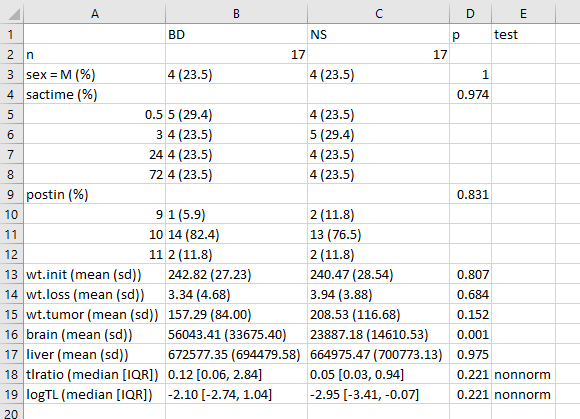
\includegraphics[width=0.9\linewidth]{images/bb-table1inExcel}

One thing I would definitely clean up here, in practice, is to change
the presentation of the \emph{p} value for \texttt{sex} from 1 to
\textgreater{} 0.99, or just omit it altogether. I'd also drop the
\texttt{computer-ese} where possible, add units for the measures, round
\textbf{a lot}, identify the outcomes carefully, and use notes to
indicate deviations from the main approach.

\subsection{A More Finished Version (after Cleanup in
Word)}\label{a-more-finished-version-after-cleanup-in-word}

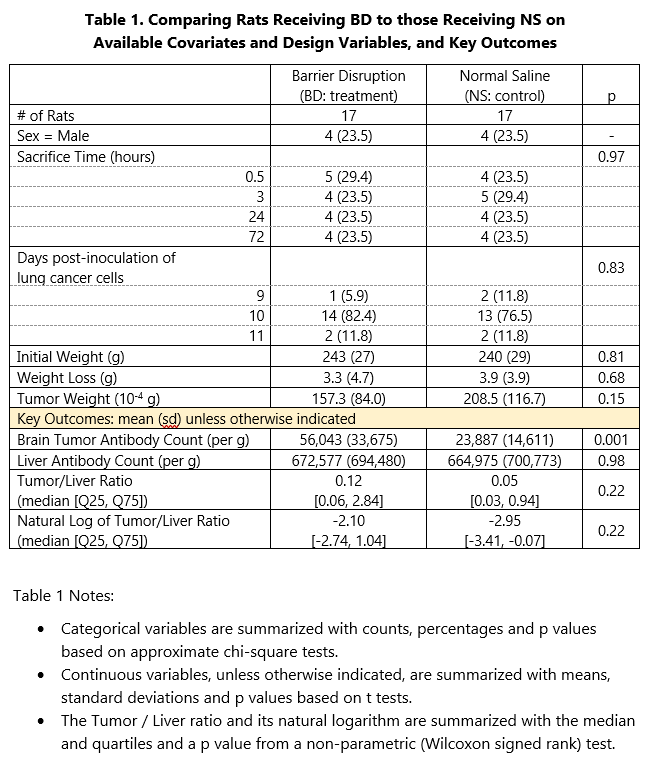
\includegraphics[width=0.95\linewidth]{images/bb-table1inWord}

\chapter{Linear Regression on a small SMART data
set}\label{linear-regression-on-a-small-smart-data-set}

\section{BRFSS and SMART}\label{brfss-and-smart}

The Centers for Disease Control analyzes Behavioral Risk Factor
Surveillance System (BRFSS) survey data for specific metropolitan and
micropolitan statistical areas (MMSAs) in a program called the
\href{https://www.cdc.gov/brfss/smart/Smart_data.htm}{Selected
Metropolitan/Micropolitan Area Risk Trends of BRFSS} (SMART BRFSS.)

In this work, we will focus on
\href{https://www.cdc.gov/brfss/smart/smart_2016.html}{data from the
2016 SMART}, and in particular on data from the Cleveland-Elyria, OH,
Metropolitan Statistical Area. The purpose of this survey is to provide
localized health information that can help public health practitioners
identify local emerging health problems, plan and evaluate local
responses, and efficiently allocate resources to specific needs.

\subsection{Key resources}\label{key-resources}

\begin{itemize}
\tightlist
\item
  the full data are available in the form of the 2016 SMART BRFSS MMSA
  Data, found in a zipped
  \href{https://www.cdc.gov/brfss/smart/2016/MMSA2016_XPT.zip}{SAS
  Transport Format} file. The data were released in August 2017.
\item
  the
  \href{https://www.cdc.gov/brfss/smart/2016/mmsa_varlayout_16.pdf}{MMSA
  Variable Layout PDF} which simply lists the variables included in the
  data file
\item
  the
  \href{https://www.cdc.gov/brfss/annual_data/2016/pdf/2016_calculated_variables_version4.pdf}{Calculated
  Variables PDF} which describes the risk factors by data variable names
  - there is also an
  \href{https://www.cdc.gov/brfss/annual_data/2016/Summary_Matrix_16.html}{online
  summary matrix of these calculated variables}, as well.
\item
  the lengthy
  \href{https://www.cdc.gov/brfss/questionnaires/pdf-ques/2016_BRFSS_Questionnaire_FINAL.pdf}{2016
  Survey Questions PDF} which lists all questions asked as part of the
  BRFSS in 2016
\item
  the enormous
  \href{https://www.cdc.gov/brfss/annual_data/2016/pdf/codebook16_llcp.pdf}{Codebook
  for the 2016 BRFSS Survey PDF} which identifies the variables by name
  for us.
\end{itemize}

Later this term, we'll use all of those resources to help construct a
more complete data set than we'll study today. I'll also demonstrate how
I built the \texttt{smartcle1} data set that we'll use in this Chapter.

\section{\texorpdfstring{The \texttt{smartcle1} data:
Cookbook}{The smartcle1 data: Cookbook}}\label{the-smartcle1-data-cookbook}

The \texttt{smartcle1.csv} data file available on the Data and Code page
of \href{https://github.com/THOMASELOVE/432-2018}{our website} describes
information on 11 variables for 1036 respondents to the BRFSS 2016, who
live in the Cleveland-Elyria, OH, Metropolitan Statistical Area. The
variables in the \texttt{smartcle1.csv} file are listed below, along
with (in some cases) the BRFSS items that generate these responses.

\begin{longtable}[]{@{}rl@{}}
\toprule
\begin{minipage}[b]{0.14\columnwidth}\raggedleft\strut
Variable\strut
\end{minipage} & \begin{minipage}[b]{0.74\columnwidth}\raggedright\strut
Description\strut
\end{minipage}\tabularnewline
\midrule
\endhead
\begin{minipage}[t]{0.14\columnwidth}\raggedleft\strut
\texttt{SEQNO}\strut
\end{minipage} & \begin{minipage}[t]{0.74\columnwidth}\raggedright\strut
respondent identification number (all begin with 2016)\strut
\end{minipage}\tabularnewline
\begin{minipage}[t]{0.14\columnwidth}\raggedleft\strut
\texttt{physhealth}\strut
\end{minipage} & \begin{minipage}[t]{0.74\columnwidth}\raggedright\strut
Now thinking about your physical health, which includes physical illness
and injury, for how many days during the past 30 days was your physical
health not good?\strut
\end{minipage}\tabularnewline
\begin{minipage}[t]{0.14\columnwidth}\raggedleft\strut
\texttt{menthealth}\strut
\end{minipage} & \begin{minipage}[t]{0.74\columnwidth}\raggedright\strut
Now thinking about your mental health, which includes stress,
depression, and problems with emotions, for how many days during the
past 30 days was your mental health not good?\strut
\end{minipage}\tabularnewline
\begin{minipage}[t]{0.14\columnwidth}\raggedleft\strut
\texttt{poorhealth}\strut
\end{minipage} & \begin{minipage}[t]{0.74\columnwidth}\raggedright\strut
During the past 30 days, for about how many days did poor physical or
mental health keep you from doing your usual activities, such as
self-care, work, or recreation?\strut
\end{minipage}\tabularnewline
\begin{minipage}[t]{0.14\columnwidth}\raggedleft\strut
\texttt{genhealth}\strut
\end{minipage} & \begin{minipage}[t]{0.74\columnwidth}\raggedright\strut
Would you say that in general, your health is \ldots{} (five categories:
Excellent, Very Good, Good, Fair or Poor)\strut
\end{minipage}\tabularnewline
\begin{minipage}[t]{0.14\columnwidth}\raggedleft\strut
\texttt{bmi}\strut
\end{minipage} & \begin{minipage}[t]{0.74\columnwidth}\raggedright\strut
Body mass index, in kg/m\textsuperscript{2}\strut
\end{minipage}\tabularnewline
\begin{minipage}[t]{0.14\columnwidth}\raggedleft\strut
\texttt{female}\strut
\end{minipage} & \begin{minipage}[t]{0.74\columnwidth}\raggedright\strut
Sex, 1 = female, 0 = male\strut
\end{minipage}\tabularnewline
\begin{minipage}[t]{0.14\columnwidth}\raggedleft\strut
\texttt{internet30}\strut
\end{minipage} & \begin{minipage}[t]{0.74\columnwidth}\raggedright\strut
Have you used the internet in the past 30 days? (1 = yes, 0 = no)\strut
\end{minipage}\tabularnewline
\begin{minipage}[t]{0.14\columnwidth}\raggedleft\strut
\texttt{exerany}\strut
\end{minipage} & \begin{minipage}[t]{0.74\columnwidth}\raggedright\strut
During the past month, other than your regular job, did you participate
in any physical activities or exercises such as running, calisthenics,
golf, gardening, or walking for exercise? (1 = yes, 0 = no)\strut
\end{minipage}\tabularnewline
\begin{minipage}[t]{0.14\columnwidth}\raggedleft\strut
\texttt{sleephrs}\strut
\end{minipage} & \begin{minipage}[t]{0.74\columnwidth}\raggedright\strut
On average, how many hours of sleep do you get in a 24-hour
period?\strut
\end{minipage}\tabularnewline
\begin{minipage}[t]{0.14\columnwidth}\raggedleft\strut
\texttt{alcdays}\strut
\end{minipage} & \begin{minipage}[t]{0.74\columnwidth}\raggedright\strut
How many days during the past 30 days did you have at least one drink of
any alcoholic beverage such as beer, wine, a malt beverage or
liquor?\strut
\end{minipage}\tabularnewline
\bottomrule
\end{longtable}

\begin{Shaded}
\begin{Highlighting}[]
\KeywordTok{str}\NormalTok{(smartcle1)}
\end{Highlighting}
\end{Shaded}

\begin{verbatim}
Classes 'tbl_df', 'tbl' and 'data.frame':   1036 obs. of  11 variables:
 $ SEQNO     : num  2.02e+09 2.02e+09 2.02e+09 2.02e+09 2.02e+09 ...
 $ physhealth: int  0 0 1 0 5 4 2 2 0 0 ...
 $ menthealth: int  0 0 5 0 0 18 0 3 0 0 ...
 $ poorhealth: int  NA NA 0 NA 0 6 0 0 NA NA ...
 $ genhealth : Factor w/ 5 levels "1_Excellent",..: 2 1 2 3 1 2 3 3 2 3 ...
 $ bmi       : num  26.7 23.7 26.9 21.7 24.1 ...
 $ female    : int  1 0 0 1 0 0 1 1 0 0 ...
 $ internet30: int  1 1 1 1 1 1 1 1 1 1 ...
 $ exerany   : int  1 1 0 1 1 1 1 1 1 0 ...
 $ sleephrs  : int  6 6 8 9 7 5 9 7 7 7 ...
 $ alcdays   : int  1 4 4 3 2 28 4 2 4 25 ...
\end{verbatim}

\section{\texorpdfstring{\texttt{smartcle2}: Omitting Missing
Observations: Complete-Case
Analyses}{smartcle2: Omitting Missing Observations: Complete-Case Analyses}}\label{smartcle2-omitting-missing-observations-complete-case-analyses}

For the purpose of fitting our first few models, we will eliminate the
missingness problem, and look only at the \emph{complete cases} in our
\texttt{smartcle1} data.

To inspect the missingness in our data, we might consider using the
\texttt{skim} function from the \texttt{skimr} package. We'll exclude
the respondent identifier code (\texttt{SEQNO}) from this summary as
uninteresting.

\begin{Shaded}
\begin{Highlighting}[]
\KeywordTok{skim_with}\NormalTok{(}\DataTypeTok{numeric =} \KeywordTok{list}\NormalTok{(}\DataTypeTok{hist =} \OtherTok{NULL}\NormalTok{), }\DataTypeTok{integer =} \KeywordTok{list}\NormalTok{(}\DataTypeTok{hist =} \OtherTok{NULL}\NormalTok{))}
\NormalTok{## above line eliminates the sparkline histograms}
\NormalTok{## it can be commented out when working in the console,}
\NormalTok{## but I need it to produce the Notes without errors right now}

\NormalTok{smartcle1 }\OperatorTok\StringTok{ }
\StringTok{    }\KeywordTok{skim}\NormalTok{(}\OperatorTok{-}\NormalTok{SEQNO)}
\end{Highlighting}
\end{Shaded}

\begin{verbatim}
Skim summary statistics
 n obs: 1036 
 n variables: 11 

Variable type: factor 
  variable missing complete    n n_unique
 genhealth       3     1033 1036        5
                             top_counts ordered
 2_V: 350, 3_G: 344, 1_E: 173, 4_F: 122   FALSE

Variable type: integer 
   variable missing complete    n mean   sd p0 p25 median p75 p100
    alcdays      46      990 1036 4.65 8.05  0   0      1   4   30
    exerany       3     1033 1036 0.76 0.43  0   1      1   1    1
     female       0     1036 1036 0.6  0.49  0   0      1   1    1
 internet30       6     1030 1036 0.81 0.39  0   1      1   1    1
 menthealth      11     1025 1036 2.72 6.82  0   0      0   2   30
 physhealth      17     1019 1036 3.97 8.67  0   0      0   2   30
 poorhealth     543      493 1036 4.07 8.09  0   0      0   3   30
   sleephrs       8     1028 1036 7.02 1.53  1   6      7   8   20

Variable type: numeric 
 variable missing complete    n  mean   sd    p0  p25 median   p75  p100
      bmi      84      952 1036 27.89 6.47 12.71 23.7  26.68 30.53 66.06
\end{verbatim}

Now, we'll create a new tibble called \texttt{smartcle2} which contains
every variable except \texttt{poorhealth}, and which includes all
respondents with complete data on the variables (other than
\texttt{poorhealth}). We'll store those observations with complete data
in the \texttt{smartcle2} tibble.

\begin{Shaded}
\begin{Highlighting}[]
\NormalTok{smartcle2 <-}\StringTok{ }\NormalTok{smartcle1 }\OperatorTok\StringTok{ }
\StringTok{    }\KeywordTok{select}\NormalTok{(}\OperatorTok{-}\NormalTok{poorhealth) }\OperatorTok
\StringTok{    }\KeywordTok{filter}\NormalTok{(}\KeywordTok{complete.cases}\NormalTok{(.))}

\NormalTok{smartcle2}
\end{Highlighting}
\end{Shaded}

\begin{verbatim}
# A tibble: 896 x 10
     SEQNO physhealth menthealth genhealth   bmi female internet30 exerany
     <dbl>      <int>      <int> <fct>     <dbl>  <int>      <int>   <int>
 1  2.02e9          0          0 2_VeryGo~  26.7      1          1       1
 2  2.02e9          0          0 1_Excell~  23.7      0          1       1
 3  2.02e9          1          5 2_VeryGo~  26.9      0          1       0
 4  2.02e9          0          0 3_Good     21.7      1          1       1
 5  2.02e9          5          0 1_Excell~  24.1      0          1       1
 6  2.02e9          4         18 2_VeryGo~  27.6      0          1       1
 7  2.02e9          2          0 3_Good     25.7      1          1       1
 8  2.02e9          2          3 3_Good     28.5      1          1       1
 9  2.02e9          0          0 2_VeryGo~  28.6      0          1       1
10  2.02e9          0          0 3_Good     23.1      0          1       0
# ... with 886 more rows, and 2 more variables: sleephrs <int>, alcdays
#   <int>
\end{verbatim}

Note that there are only 896 respondents with \textbf{complete} data on
the 10 variables (excluding \texttt{poorhealth}) in the
\texttt{smartcle2} tibble, as compared to our original
\texttt{smartcle1} data which described 1036 respondents and 11
variables, but with lots of missing data.

\section{\texorpdfstring{Can we use \texttt{bmi} to predict
\texttt{physhealth}?}{Can we use bmi to predict physhealth?}}\label{can-we-use-bmi-to-predict-physhealth}

We'll start with an effort to predict \texttt{physhealth} using
\texttt{bmi}. A natural graph would be a scatterplot.

\begin{Shaded}
\begin{Highlighting}[]
\KeywordTok{ggplot}\NormalTok{(}\DataTypeTok{data =}\NormalTok{ smartcle2, }\KeywordTok{aes}\NormalTok{(}\DataTypeTok{x =}\NormalTok{ bmi, }\DataTypeTok{y =}\NormalTok{ physhealth)) }\OperatorTok{+}
\StringTok{    }\KeywordTok{geom_point}\NormalTok{()}
\end{Highlighting}
\end{Shaded}

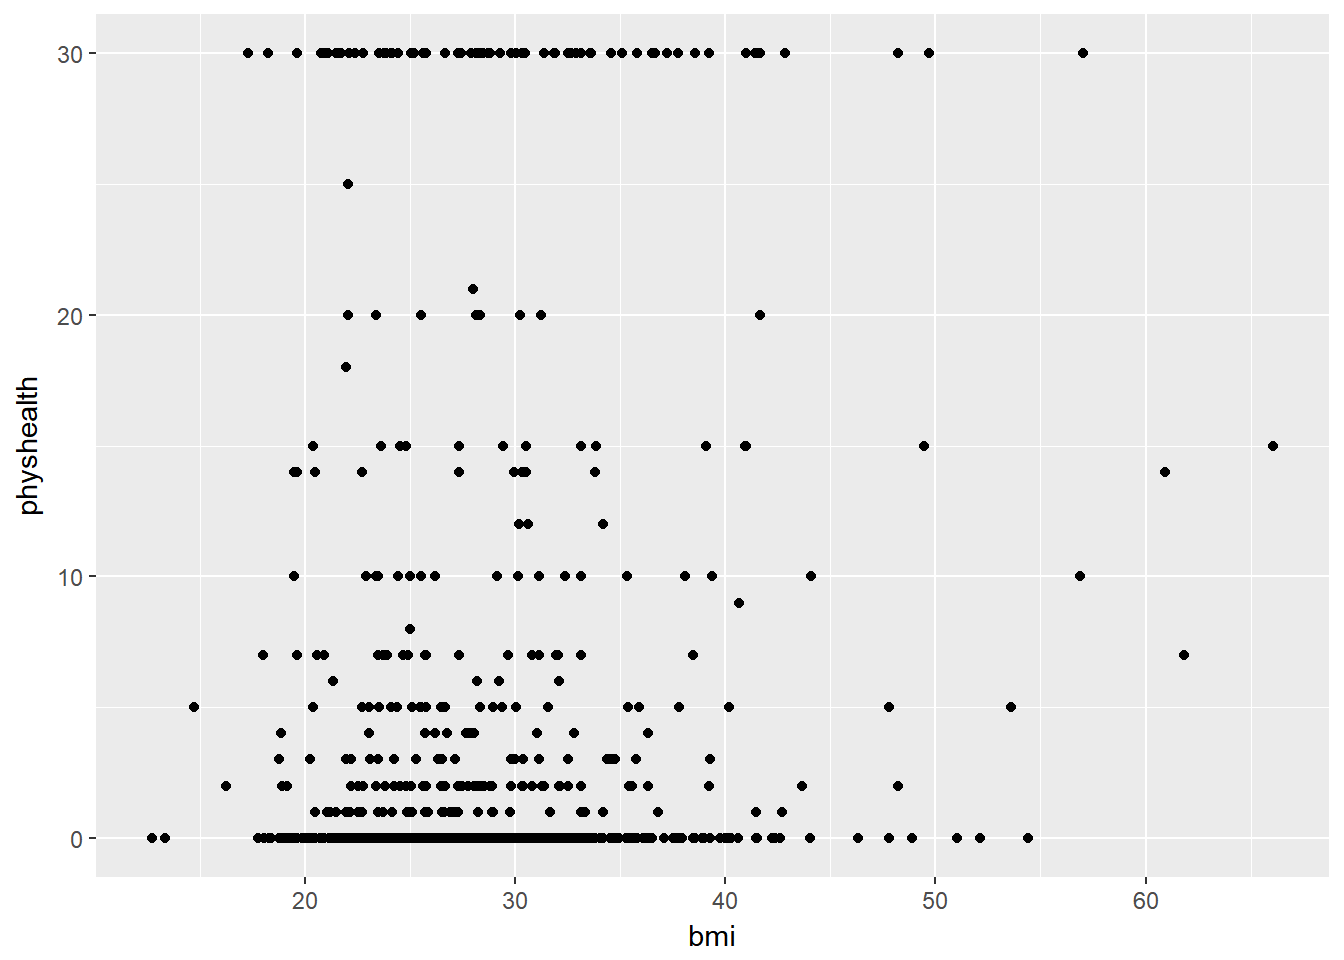
\includegraphics{bookdown-demo_files/figure-latex/scatter_physhealth_bmi_1-1.pdf}

A good question to ask ourselves here might be: ``In what BMI range can
we make a reasonable prediction of \texttt{physhealth}?''

Now, we might take the plot above and add a simple linear model \ldots{}

\begin{Shaded}
\begin{Highlighting}[]
\KeywordTok{ggplot}\NormalTok{(}\DataTypeTok{data =}\NormalTok{ smartcle2, }\KeywordTok{aes}\NormalTok{(}\DataTypeTok{x =}\NormalTok{ bmi, }\DataTypeTok{y =}\NormalTok{ physhealth)) }\OperatorTok{+}
\StringTok{    }\KeywordTok{geom_point}\NormalTok{() }\OperatorTok{+}
\StringTok{    }\KeywordTok{geom_smooth}\NormalTok{(}\DataTypeTok{method =} \StringTok{"lm"}\NormalTok{, }\DataTypeTok{se =} \OtherTok{FALSE}\NormalTok{)}
\end{Highlighting}
\end{Shaded}

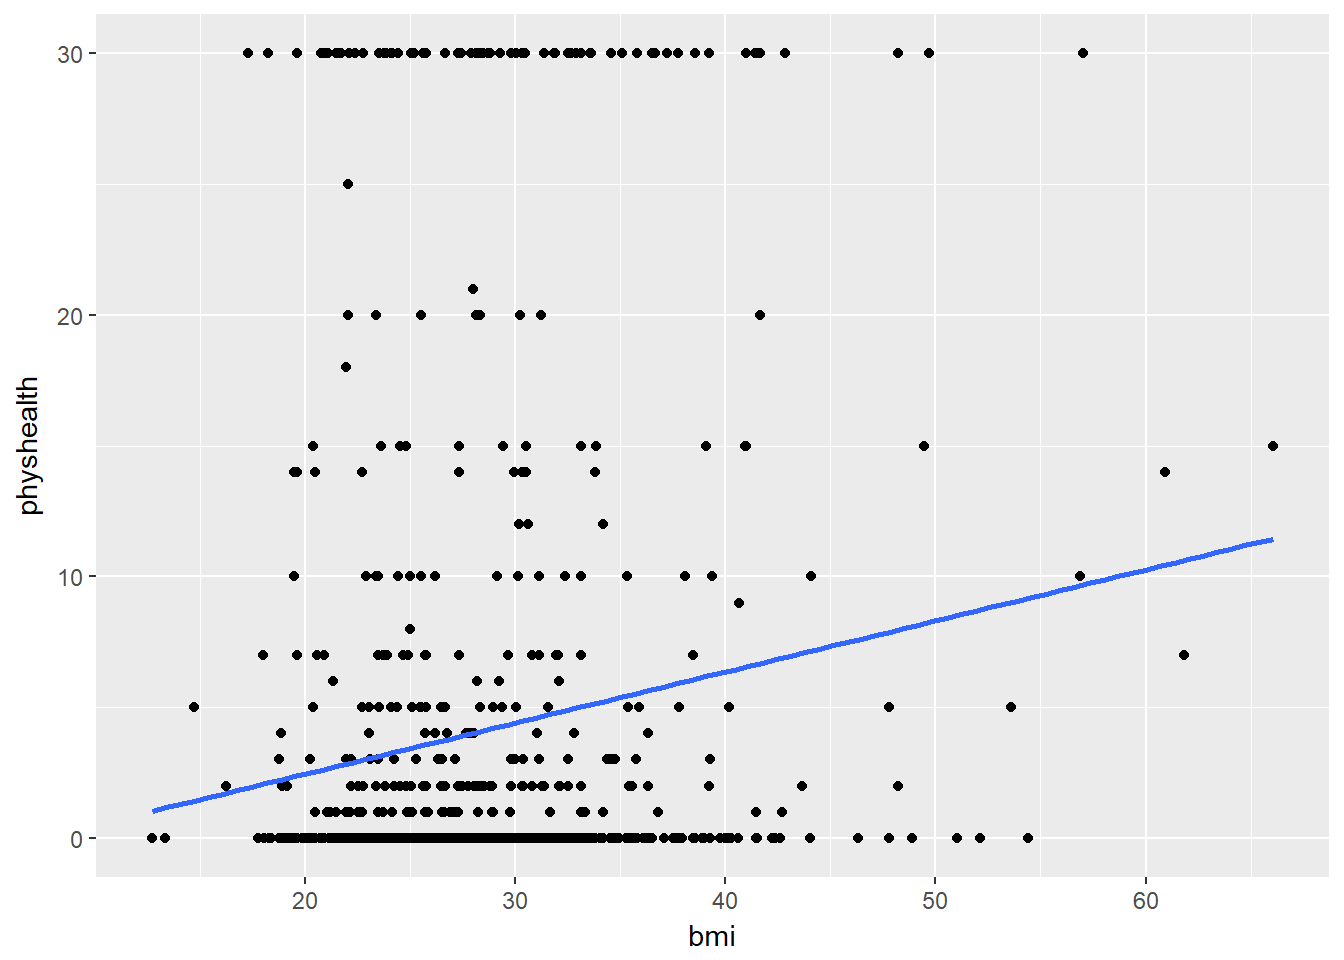
\includegraphics{bookdown-demo_files/figure-latex/c2_scatter_physhealth_bmi_2-1.pdf}

which shows the same least squares regression model that we can fit with
the \texttt{lm} command.

\subsubsection{Fitting a Simple Regression
Model}\label{fitting-a-simple-regression-model}

\begin{Shaded}
\begin{Highlighting}[]
\NormalTok{model_A <-}\StringTok{ }\KeywordTok{lm}\NormalTok{(physhealth }\OperatorTok{~}\StringTok{ }\NormalTok{bmi, }\DataTypeTok{data =}\NormalTok{ smartcle2)}

\NormalTok{model_A}
\end{Highlighting}
\end{Shaded}

\begin{verbatim}

Call:
lm(formula = physhealth ~ bmi, data = smartcle2)

Coefficients:
(Intercept)          bmi  
    -1.4514       0.1953  
\end{verbatim}

\begin{Shaded}
\begin{Highlighting}[]
\KeywordTok{summary}\NormalTok{(model_A)}
\end{Highlighting}
\end{Shaded}

\begin{verbatim}

Call:
lm(formula = physhealth ~ bmi, data = smartcle2)

Residuals:
   Min     1Q Median     3Q    Max 
-9.171 -4.057 -3.193 -1.576 28.073 

Coefficients:
            Estimate Std. Error t value Pr(>|t|)    
(Intercept) -1.45143    1.29185  -1.124    0.262    
bmi          0.19527    0.04521   4.319 1.74e-05 ***
---
Signif. codes:  0 '***' 0.001 '**' 0.01 '*' 0.05 '.' 0.1 ' ' 1

Residual standard error: 8.556 on 894 degrees of freedom
Multiple R-squared:  0.02044,   Adjusted R-squared:  0.01934 
F-statistic: 18.65 on 1 and 894 DF,  p-value: 1.742e-05
\end{verbatim}

\begin{Shaded}
\begin{Highlighting}[]
\KeywordTok{confint}\NormalTok{(model_A, }\DataTypeTok{level =} \FloatTok{0.95}\NormalTok{)}
\end{Highlighting}
\end{Shaded}

\begin{verbatim}
                 2.5 %    97.5 %
(Intercept) -3.9868457 1.0839862
bmi          0.1065409 0.2840068
\end{verbatim}

The model coefficients can be obtained by printing the model object, and
the \texttt{summary} function provides several useful descriptions of
the model's residuals, its statistical significance, and quality of fit.

\subsection{Model Summary for a Simple (One-Predictor)
Regression}\label{model-summary-for-a-simple-one-predictor-regression}

The fitted model predicts \texttt{physhealth} with the equation -1.45 +
0.195*\texttt{bmi}, as we can read off from the model coefficients.

Each of the 896 respondents included in the \texttt{smartcle2} data
makes a contribution to this model.

\subsubsection{Residuals}\label{residuals}

Suppose Harry is one of the people in that group, and Harry's data is
\texttt{bmi} = 20, and \texttt{physhealth} = 3.

\begin{itemize}
\tightlist
\item
  Harry's \emph{observed} value of \texttt{physhealth} is just the value
  we have in the data for them, in this case, observed
  \texttt{physhealth} = 3 for Harry.
\item
  Harry's \emph{fitted} or \emph{predicted} \texttt{physhealth} value is
  the result of calculating -1.45 + 0.195\emph{\texttt{bmi} for Harry.
  So, if Harry's BMI was 20, then Harry's predicted \texttt{physhealth}
  value is -1.45 + (0.195}20) = 2.45.
\item
  The \emph{residual} for Harry is then his \emph{observed} outcome
  minus his \emph{fitted} outcome, so Harry has a residual of 3 - 2.45 =
  0.55.
\item
  Graphically, a residual represents vertical distance between the
  observed point and the fitted regression line.
\item
  Points above the regression line will have positive residuals, and
  points below the regression line will have negative residuals. Points
  on the line have zero residuals.
\end{itemize}

The residuals are summarized at the top of the \texttt{summary} output
for linear model.

\begin{itemize}
\tightlist
\item
  The mean residual will always be zero in an ordinary least squares
  model, but a five number summary of the residuals is provided by the
  summary, as is an estimated standard deviation of the residuals
  (called here the Residual standard error.)
\item
  In the \texttt{smartcle2} data, the minimum residual was -9.17, so for
  one subject, the observed value was 9.17 days smaller than the
  predicted value. This means that the prediction was 9.17 days too
  large for that subject.
\item
  Similarly, the maximum residual was 28.07 days, so for one subject the
  prediction was 28.07 days too small. Not a strong performance.
\item
  In a least squares model, the residuals are assumed to follow a Normal
  distribution, with mean zero, and standard deviation (for the
  \texttt{smartcle2} data) of about 8.6 days. Thus, by the definition of
  a Normal distribution, we'd expect
\item
  about 68\% of the residuals to be between -8.6 and +8.6 days,
\item
  about 95\% of the residuals to be between -17.2 and +17.2 days,
\item
  about all (99.7\%) of the residuals to be between -25.8 and +25.8
  days.
\end{itemize}

\subsubsection{Coefficients section}\label{coefficients-section}

The \texttt{summary} for a linear model shows Estimates, Standard
Errors, t values and \emph{p} values for each coefficient fit.

\begin{itemize}
\tightlist
\item
  The Estimates are the point estimates of the intercept and slope of
  \texttt{bmi} in our model.
\item
  In this case, our estimated slope is 0.195, which implies that if
  Harry's BMI is 20 and Sally's BMI is 21, we predict that Sally's
  \texttt{physhealth} will be 0.195 days larger than Harry's.
\item
  The Standard Errors are also provided for each estimate. We can create
  rough 95\% confidence intervals by adding and subtracting two standard
  errors from each coefficient, or we can get a slightly more accurate
  answer with the \texttt{confint} function.
\item
  Here, the 95\% confidence interval for the slope of \texttt{bmi} is
  estimated to be (0.11, 0.28). This is a good measure of the
  uncertainty in the slope that is captured by our model. We are 95\%
  confident in the process of building this interval, but this doesn't
  mean we're 95\% sure that the true slope is actually in that interval.
\end{itemize}

Also available are a \emph{t} value (just the Estimate divided by the
Standard Error) and the appropriate \emph{p} value for testing the null
hypothesis that the true value of the coefficient is 0 against a
two-tailed alternative.

\begin{itemize}
\tightlist
\item
  If a slope coefficient is statistically significantly different from
  0, this implies that 0 will not be part of the uncertainty interval
  obtained through \texttt{confint}.
\item
  If the slope was zero, it would suggest that \texttt{bmi} would add no
  predictive value to the model. But that's unlikely here.
\end{itemize}

If the \texttt{bmi} slope coefficient is associated with a small
\emph{p} value, as in the case of our \texttt{model\_A}, it suggests
that the model including \texttt{bmi} is statistically significantly
better at predicting \texttt{physhealth} than the model without
\texttt{bmi}.

\begin{itemize}
\tightlist
\item
  Without \texttt{bmi} our \texttt{model\_A} would become an
  \emph{intercept-only} model, in this case, which would predict the
  mean \texttt{physhealth} for everyone, regardless of any other
  information.
\end{itemize}

\subsubsection{Model Fit Summaries}\label{model-fit-summaries}

The \texttt{summary} of a linear model also displays:

\begin{itemize}
\tightlist
\item
  The residual standard error and associated degrees of freedom for the
  residuals.
\item
  For a simple (one-predictor) least regression like this, the residual
  degrees of freedom will be the sample size minus 2.
\item
  The multiple R-squared (or coefficient of determination)
\item
  This is interpreted as the proportion of variation in the outcome
  (\texttt{physhealth}) accounted for by the model, and will always fall
  between 0 and 1 as a result.
\item
  Our model\_A accounts for a mere 2\% of the variation in
  \texttt{physhealth}.
\item
  The Adjusted R-squared value ``adjusts'' for the size of our model in
  terms of the number of coefficients included in the model.
\item
  The adjusted R-squared will always be less than the Multiple
  R-squared.
\item
  We still hope to find models with relatively large adjusted
  R\textsuperscript{2} values.
\item
  In particular, we hope to find models where the adjusted
  R\textsuperscript{2} isn't substantially less than the Multiple
  R-squared.
\item
  The adjusted R-squared is usually a better estimate of likely
  performance of our model in new data than is the Multiple R-squared.
\item
  The adjusted R-squared result is no longer interpretable as a
  proportion of anything - in fact, it can fall below 0.
\item
  We can obtain the adjusted R\textsuperscript{2} from the raw
  R\textsuperscript{2}, the number of observations \emph{N} and the
  number of predictors \emph{p} included in the model, as follows:
\end{itemize}

\[
R^2_{adj} = 1 - \frac{(1 - R^2)(N - 1)}{N - p - 1},
\]

\begin{itemize}
\tightlist
\item
  The F statistic and \emph{p} value from a global ANOVA test of the
  model.

  \begin{itemize}
  \tightlist
  \item
    Obtaining a statistically significant result here is usually pretty
    straightforward, since the comparison is between our model, and a
    model which simply predicts the mean value of the outcome for
    everyone.
  \item
    In a simple (one-predictor) linear regression like this, the t
    statistic for the slope is just the square root of the F statistic,
    and the resulting \emph{p} values for the slope's t test and for the
    global F test will be identical.
  \end{itemize}
\item
  To see the complete ANOVA F test for this model, we can run
  \texttt{anova(model\_A)}.
\end{itemize}

\begin{Shaded}
\begin{Highlighting}[]
\KeywordTok{anova}\NormalTok{(model_A)}
\end{Highlighting}
\end{Shaded}

\begin{verbatim}
Analysis of Variance Table

Response: physhealth
           Df Sum Sq Mean Sq F value    Pr(>F)    
bmi         1   1366  1365.5  18.655 1.742e-05 ***
Residuals 894  65441    73.2                      
---
Signif. codes:  0 '***' 0.001 '**' 0.01 '*' 0.05 '.' 0.1 ' ' 1
\end{verbatim}

\subsection{\texorpdfstring{Using the \texttt{broom}
package}{Using the broom package}}\label{using-the-broom-package}

The \texttt{broom} package has three functions of particular use in a
linear regression model:

\begin{itemize}
\tightlist
\item
  \texttt{tidy} builds a data frame/tibble containing information about
  the coefficients in the model, their standard errors, t statistics and
  \emph{p} values.
\end{itemize}

\begin{Shaded}
\begin{Highlighting}[]
\KeywordTok{tidy}\NormalTok{(model_A)}
\end{Highlighting}
\end{Shaded}

\begin{verbatim}
         term   estimate  std.error statistic      p.value
1 (Intercept) -1.4514298 1.29185199 -1.123526 2.615156e-01
2         bmi  0.1952739 0.04521145  4.319125 1.741859e-05
\end{verbatim}

\begin{itemize}
\tightlist
\item
  \texttt{glance} builds a data frame/tibble containing summary
  statistics about the model, including
\item
  the (raw) multiple R\textsuperscript{2} and adjusted R\^{}2
\item
  \texttt{sigma} which is the residual standard error
\item
  the F \texttt{statistic}, \texttt{p.value} model \texttt{df} and
  \texttt{df.residual} associated with the global ANOVA test, plus
\item
  several statistics that will be useful in comparing models down the
  line:
\item
  the model's log likelihood function value, \texttt{logLik}
\item
  the model's Akaike's Information Criterion value, \texttt{AIC}
\item
  the model's Bayesian Information Criterion value, \texttt{BIC}
\item
  and the model's \texttt{deviance} statistic
\end{itemize}

\begin{Shaded}
\begin{Highlighting}[]
\KeywordTok{glance}\NormalTok{(model_A)}
\end{Highlighting}
\end{Shaded}

\begin{verbatim}
   r.squared adj.r.squared    sigma statistic      p.value df    logLik
1 0.02044019    0.01934449 8.555737  18.65484 1.741859e-05  2 -3193.723
       AIC     BIC deviance df.residual
1 6393.446 6407.84 65441.36         894
\end{verbatim}

\begin{itemize}
\tightlist
\item
  \texttt{augment} builds a data frame/tibble which adds fitted values,
  residuals and other diagnostic summaries that describe each
  observation to the original data used to fit the model, and this
  includes
\item
  \texttt{.fitted} and \texttt{.resid}, the fitted and residual values,
  in addition to
\item
  \texttt{.hat}, the leverage value for this observation
\item
  \texttt{.cooksd}, the Cook's distance measure of \emph{influence} for
  this observation
\item
  \texttt{.stdresid}, the standardized residual (think of this as a
  z-score - a measure of the residual divided by its associated standard
  deviation \texttt{.sigma})
\item
  and \texttt{se.fit} which will help us generate prediction intervals
  for the model downstream
\end{itemize}

Note that each of the new columns begins with \texttt{.} to avoid
overwriting any data.

\begin{Shaded}
\begin{Highlighting}[]
\KeywordTok{augment}\NormalTok{(model_A)}
\end{Highlighting}
\end{Shaded}

\begin{verbatim}
    physhealth   bmi   .fitted   .se.fit      .resid        .hat   .sigma
1            0 26.69  3.760430 0.2907252 -3.76043009 0.001154651 8.559600
2            0 23.70  3.176561 0.3422908 -3.17656119 0.001600574 8.559865
3            1 26.92  3.805343 0.2890054 -2.80534308 0.001141030 8.560010
4            0 21.66  2.778202 0.4005101 -2.77820248 0.002191352 8.560020
5            5 24.09  3.252718 0.3329154  1.74728200 0.001514095 8.560326
6            4 27.64  3.945940 0.2860087  0.05405972 0.001117490 8.560526
7            2 25.71  3.569062 0.3019825 -1.56906169 0.001245801 8.560365
8            2 28.52  4.117781 0.2873552 -2.11778129 0.001128037 8.560232
9            0 28.63  4.139261 0.2879099 -4.13926142 0.001132396 8.559404
10           0 23.10  3.059397 0.3579331 -3.05939686 0.001750205 8.559913
11           0 26.60  3.742855 0.2914965 -3.74285544 0.001160785 8.559608
12          30 20.76  2.602456 0.4299951 27.39754402 0.002525877 8.511164
13           0 21.66  2.778202 0.4005101 -2.77820248 0.002191352 8.560020
14           3 32.51  4.896924 0.3546724 -1.89692407 0.001718462 8.560290
15           0 32.60  4.914499 0.3570966 -4.91449872 0.001742034 8.558943
16           0 18.27  2.116224 0.5195177 -2.11622402 0.003687108 8.560232
17           0 21.20  2.688376 0.4153437 -2.68837649 0.002356680 8.560052
18           0 33.13  5.017994 0.3719552 -5.01799388 0.001890021 8.558876
19           3 27.14  3.848303 0.2877025 -0.84830334 0.001130765 8.560479
20           0 13.34  1.153524 0.7162199 -1.15352380 0.007007739 8.560438
21           0 26.60  3.742855 0.2914965 -3.74285544 0.001160785 8.559608
22           0 36.37  5.650681 0.4791047 -5.65068125 0.003135784 8.558431
23           0 27.32  3.883453 0.2868888 -3.88345263 0.001124378 8.559538
24           1 21.03  2.655180 0.4209535 -1.65517993 0.002420770 8.560346
25           0 28.04  4.024050 0.2859361 -4.02404983 0.001116923 8.559465
26           0 26.68  3.758477 0.2908082 -3.75847735 0.001155310 8.559601
27           1 21.17  2.682518 0.4163289 -1.68251827 0.002367872 8.560340
28           6 32.10  4.816862 0.3440220  1.18313822 0.001616805 8.560434
29           0 21.19  2.686424 0.4156719 -2.68642375 0.002360405 8.560053
30           0 27.09  3.838540 0.2879690 -3.83853964 0.001132861 8.559561
31           0 27.32  3.883453 0.2868888 -3.88345263 0.001124378 8.559538
32           0 31.41  4.682123 0.3276877 -4.68212280 0.001466917 8.559090
33           0 12.71  1.030501 0.7424237 -1.03050125 0.007529893 8.560456
34           0 31.83  4.764138 0.3373811 -4.76413783 0.001554986 8.559039
35           0 18.96  2.250963 0.4937660 -2.25096300 0.003330639 8.560193
36           0 25.90  3.606164 0.2993209 -3.60616373 0.001223937 8.559674
37           0 37.86  5.941639 0.5346811 -5.94163933 0.003905483 8.558207
38           0 23.92  3.219521 0.3369208 -3.21952144 0.001550746 8.559847
39           2 28.04  4.024050 0.2859361 -2.02404983 0.001116923 8.560258
40           0 24.11  3.256623 0.3324527 -3.25662348 0.001509889 8.559831
41           0 20.32  2.516535 0.4450535 -2.51653548 0.002705887 8.560110
42           3 30.38  4.480991 0.3076073 -1.48099071 0.001292642 8.560382
43           0 28.63  4.139261 0.2879099 -4.13926142 0.001132396 8.559404
44           1 22.50  2.942233 0.3748880 -1.94223253 0.001919943 8.560279
45           0 25.67  3.561251 0.3025709 -3.56125073 0.001250661 8.559695
46           0 26.31  3.686226 0.2943507 -3.68622602 0.001183628 8.559636
47           0 30.48  4.500518 0.3093068 -4.50051809 0.001306965 8.559199
48          30 40.97  6.548941 0.6578200 23.45105891 0.005911522 8.524265
49           0 26.66  3.754572 0.2909762 -3.75457187 0.001156645 8.559603
50           0 18.76  2.211908 0.5011666 -2.21190822 0.003431227 8.560205
51           0 29.44  4.297433 0.2945592 -4.29743326 0.001185306 8.559316
52           0 22.35  2.912941 0.3793115 -2.91294145 0.001965518 8.559970
53           0 29.15  4.240804 0.2916680 -4.24080383 0.001162152 8.559348
54           0 20.37  2.526299 0.4433231 -2.52629917 0.002684887 8.560107
55           0 28.79  4.170505 0.2888677 -4.17050524 0.001139943 8.559387
56          14 33.80  5.148827 0.3920310  8.85117262 0.002099549 8.555389
57           0 19.29  2.315403 0.4816776 -2.31540338 0.003169553 8.560174
58           2 22.18  2.879745 0.3844078 -0.87974489 0.002018690 8.560475
59           2 25.61  3.549534 0.3034716 -1.54953430 0.001258118 8.560369
60           2 25.05  3.440181 0.3128889 -1.44018093 0.001337413 8.560390
61           0 33.66  5.121489 0.3877264 -5.12148903 0.002053695 8.558807
62           0 25.83  3.592495 0.3002756 -3.59249455 0.001231758 8.559681
63           3 21.97  2.838737 0.3908203  0.16126262 0.002086601 8.560524
64           0 25.76  3.578825 0.3012606 -3.57882538 0.001239852 8.559687
65          30 25.18  3.465567 0.3105443 26.53443347 0.001317444 8.514289
66           0 28.47  4.108018 0.2871312 -4.10801760 0.001126279 8.559421
67           0 31.50  4.699697 0.3296968 -4.69969745 0.001484960 8.559079
68          30 31.39  4.678217 0.3272465 25.32178268 0.001462969 8.518423
69           0 19.49  2.354458 0.4744297 -2.35445816 0.003074886 8.560162
70           1 27.28  3.875642 0.2870499 -2.87564168 0.001125641 8.559984
71           0 29.16  4.242757 0.2917584 -4.24275657 0.001162872 8.559347
72           0 32.18  4.832484 0.3460479 -4.83248369 0.001635903 8.558996
73           0 22.50  2.942233 0.3748880 -2.94223253 0.001919943 8.559958
74           0 40.09  6.377100 0.6222261 -6.37710008 0.005289098 8.557851
75           0 44.02  7.144526 0.7843095 -7.14452643 0.008403499 8.557158
76           0 24.19  3.272245 0.3306201 -3.27224539 0.001493289 8.559824
77           0 34.10  5.207410 0.4014359 -5.20740954 0.002201494 8.558748
78           7 32.02  4.801240 0.3420223  2.19876013 0.001598064 8.560209
79          15 27.31  3.881500 0.2869280 11.11850010 0.001124685 8.552427
80           0 19.88  2.430615 0.4604790 -2.43061497 0.002896709 8.560138
81           0 23.56  3.149223 0.3458137 -3.14922285 0.001633689 8.559876
82           0 23.60  3.157034 0.3447990 -3.15703380 0.001624116 8.559873
83           3 39.28  6.218928 0.5899372 -3.21892824 0.004754411 8.559845
84           0 20.49  2.549732 0.4391899 -2.54973204 0.002635056 8.560099
85           0 24.16  3.266387 0.3313039 -3.26638717 0.001499472 8.559827
86           0 42.21  6.791081 0.7087322 -6.79108070 0.006861980 8.557488
87           0 27.47  3.912744 0.2863856 -3.91274372 0.001120437 8.559523
88           0 28.35  4.084585 0.2866656 -4.08458473 0.001122629 8.559433
89           2 26.66  3.754572 0.2909762 -1.75457187 0.001156645 8.560324
90           0 27.01  3.822918 0.2884316 -3.82291773 0.001136504 8.559569
91           0 24.79  3.389410 0.3178525 -3.38940972 0.001380182 8.559773
92           0 25.76  3.578825 0.3012606 -3.57882538 0.001239852 8.559687
93           0 24.91  3.412843 0.3155169 -3.41284258 0.001359973 8.559763
94           0 24.33  3.299584 0.3274846 -3.29958373 0.001465099 8.559813
95           0 31.01  4.604013 0.3192334 -4.60401325 0.001392201 8.559137
96           1 31.65  4.728989 0.3331288 -3.72898853 0.001516036 8.559615
97           2 27.46  3.910791 0.2864142 -1.91079098 0.001120661 8.560287
98           0 27.38  3.895169 0.2866684 -3.89516907 0.001122651 8.559532
99           1 22.73  2.987146 0.3682447 -1.98714553 0.001852500 8.560267
100         30 25.61  3.549534 0.3034716 26.45046570 0.001258118 8.514585
101          0 22.49  2.940280 0.3751807 -2.94027980 0.001922942 8.559959
102          0 26.49  3.721375 0.2925132 -3.72137531 0.001168897 8.559619
103          0 54.40  9.171469 1.2332475 -9.17146930 0.020777134 8.554906
104         30 22.08  2.860218 0.3874456 27.13978250 0.002050721 8.512114
105          2 31.39  4.678217 0.3272465 -2.67821732 0.001462969 8.560056
106          0 27.47  3.912744 0.2863856 -3.91274372 0.001120437 8.559523
107         25 22.02  2.848501 0.3892821 22.15149893 0.002070208 8.528305
108          1 33.13  5.017994 0.3719552 -4.01799388 0.001890021 8.559468
109          0 26.51  3.725281 0.2923223 -3.72528079 0.001167372 8.559617
110          7 25.71  3.569062 0.3019825  3.43093831 0.001245801 8.559755
111          0 27.31  3.881500 0.2869280 -3.88149990 0.001124685 8.559539
112          0 21.66  2.778202 0.4005101 -2.77820248 0.002191352 8.560020
113          0 35.36  5.453455 0.4432954 -5.45345463 0.002684550 8.558575
114          2 24.25  3.283962 0.3292651 -1.28396182 0.001481073 8.560418
115          0 21.16  2.680566 0.4166577 -2.68056554 0.002371614 8.560055
116         15 23.62  3.160939 0.3442940 11.83906072 0.001619363 8.551338
117          0 25.03  3.436275 0.3132578 -3.43627545 0.001340569 8.559752
118          0 26.87  3.795579 0.2893483 -3.79557939 0.001143739 8.559582
119         30 25.05  3.440181 0.3128889 26.55981907 0.001337413 8.514200
120          0 27.40  3.899075 0.2866006 -3.89907454 0.001122120 8.559530
121          0 29.02  4.215418 0.2905548 -4.21541823 0.001153297 8.559362
122          0 19.32  2.321262 0.4805865 -2.32126160 0.003155211 8.560172
123         30 17.30  1.926808 0.5566620 28.07319164 0.004233195 8.508602
124          0 27.83  3.983042 0.2858316 -3.98304231 0.001116106 8.559487
125          0 29.73  4.354063 0.2979997 -4.35406268 0.001213157 8.559284
126          0 21.34  2.715715 0.4107744 -2.71571483 0.002305111 8.560042
127          0 27.77  3.971326 0.2858596 -3.97132588 0.001116326 8.559493
128          0 26.31  3.686226 0.2943507 -3.68622602 0.001183628 8.559636
129          2 31.39  4.678217 0.3272465 -2.67821732 0.001462969 8.560056
130          0 32.51  4.896924 0.3546724 -4.89692407 0.001718462 8.558955
131         30 34.55  5.295283 0.4159739 24.70471722 0.002363836 8.520418
132          0 25.11  3.451897 0.3117952 -3.45189736 0.001328079 8.559745
133         14 19.61  2.377891 0.4701109 11.62210898 0.003019157 8.551660
134          0 22.50  2.942233 0.3748880 -2.94223253 0.001919943 8.559958
135         15 24.80  3.391362 0.3176549 11.60863754 0.001378467 8.551695
136          0 24.66  3.364024 0.3204671 -3.36402411 0.001402982 8.559785
137          0 34.70  5.324574 0.4209268 -5.32457387 0.002420463 8.558667
138          5 26.68  3.758477 0.2908082  1.24152265 0.001155310 8.560425
139         15 24.54  3.340591 0.3229568 11.65940875 0.001424866 8.551617
140          0 28.93  4.197844 0.2898514 -4.19784358 0.001147720 8.559372
141          0 29.82  4.371637 0.2991762 -4.37163733 0.001222755 8.559274
142          0 31.99  4.795382 0.3412793 -4.79538165 0.001591128 8.559019
143          4 27.83  3.983042 0.2858316  0.01695769 0.001116106 8.560526
144          2 28.25  4.065057 0.2863555 -2.06505734 0.001120202 8.560247
145          1 20.49  2.549732 0.4391899 -1.54973204 0.002635056 8.560368
146          3 26.33  3.690131 0.2941359 -0.69013149 0.001181902 8.560495
147         30 23.87  3.209758 0.3381230 26.79024225 0.001561833 8.513379
148          0 30.78  4.559100 0.3147401 -4.55910026 0.001353285 8.559164
149          5 25.76  3.578825 0.3012606  1.42117462 0.001239852 8.560394
150          5 23.54  3.145317 0.3463235  1.85468263 0.001638510 8.560300
151          0 42.38  6.824277 0.7157721 -6.82427726 0.006998979 8.557458
152         30 33.60  5.109773 0.3858987 24.89022740 0.002034379 8.519826
153         10 23.39  3.116026 0.3501976  6.88397371 0.001675373 8.557420
154          0 28.25  4.065057 0.2863555 -4.06505734 0.001120202 8.559444
155          4 18.83  2.225577 0.4985703  1.77442260 0.003395767 8.560319
156          7 18.00  2.063500 0.5297538  4.93649992 0.003833834 8.558926
157          0 29.49  4.307197 0.2951137 -4.30719695 0.001189773 8.559311
158         30 30.04  4.414598 0.3022636 25.58540241 0.001248122 8.517549
159          0 25.40  3.508527 0.3067922 -3.50852679 0.001285801 8.559720
160          2 28.04  4.024050 0.2859361 -2.02404983 0.001116923 8.560258
161          2 31.32  4.664548 0.3257171 -2.66454815 0.001449327 8.560061
162          0 24.92  3.414795 0.3153257 -3.41479532 0.001358325 8.559762
163          5 35.89  5.556950 0.4618697 -0.55694978 0.002914232 8.560505
164          2 28.25  4.065057 0.2863555 -2.06505734 0.001120202 8.560247
165         30 39.24  6.211117 0.5883558 23.78888272 0.004728956 8.523255
166          0 32.44  4.883255 0.3528079 -4.88325490 0.001700441 8.558963
167          2 29.80  4.367732 0.2989104 -2.36773186 0.001220583 8.560159
168          0 23.82  3.199994 0.3393361 -3.19999406 0.001573060 8.559855
169          0 23.92  3.219521 0.3369208 -3.21952144 0.001550746 8.559847
170          0 23.54  3.145317 0.3463235 -3.14531737 0.001638510 8.559878
171          0 27.14  3.848303 0.2877025 -3.84830334 0.001130765 8.559556
172          7 33.15  5.021899 0.3725345  1.97810065 0.001895912 8.560269
173         10 19.49  2.354458 0.4744297  7.64554184 0.003074886 8.556690
174         30 32.51  4.896924 0.3546724 25.10307593 0.001718462 8.519138
175          0 25.73  3.572967 0.3016919 -3.57296717 0.001243404 8.559690
176         30 26.68  3.758477 0.2908082 26.24152265 0.001155310 8.515315
177          0 23.90  3.215616 0.3374004 -3.21561597 0.001555164 8.559848
178          3 18.78  2.215814 0.5004241  0.78418630 0.003421068 8.560485
179          0 32.10  4.816862 0.3440220 -4.81686178 0.001616805 8.559006
180         30 30.31  4.467322 0.3064517 25.53267847 0.001282949 8.517725
181         30 36.51  5.678020 0.4841993 24.32198041 0.003202827 8.521622
182          0 23.99  3.233191 0.3352560 -3.23319061 0.001535459 8.559841
183          0 24.84  3.399173 0.3168701 -3.39917341 0.001371664 8.559769
184          0 23.04  3.047680 0.3595725 -3.04768043 0.001766274 8.559917
185          0 22.73  2.987146 0.3682447 -2.98714553 0.001852500 8.559941
186          0 25.83  3.592495 0.3002756 -3.59249455 0.001231758 8.559681
187          0 31.47  4.693839 0.3290229 -4.69383924 0.001478895 8.559083
188          0 29.62  4.332583 0.2966312 -4.33258256 0.001202040 8.559296
189         10 33.13  5.017994 0.3719552  4.98200612 0.001890021 8.558899
190          0 25.71  3.569062 0.3019825 -3.56906169 0.001245801 8.559692
191          0 29.23  4.256426 0.2924097 -4.25642574 0.001168070 8.559339
192          0 33.66  5.121489 0.3877264 -5.12148903 0.002053695 8.558807
193          0 29.99  4.404834 0.3015359 -4.40483389 0.001242119 8.559255
194          0 26.66  3.754572 0.2909762 -3.75457187 0.001156645 8.559603
195          0 26.51  3.725281 0.2923223 -3.72528079 0.001167372 8.559617
196          0 38.51  6.068567 0.5597375 -6.06856735 0.004280101 8.558106
197          0 22.28  2.899272 0.3813995 -2.89927228 0.001987217 8.559975
198          0 22.89  3.018389 0.3637271 -3.01838935 0.001807326 8.559929
199          0 31.84  4.766091 0.3376215 -4.76609057 0.001557203 8.559038
200          0 22.18  2.879745 0.3844078 -2.87974489 0.002018690 8.559982
201          2 30.31  4.467322 0.3064517 -2.46732153 0.001282949 8.560127
202         14 30.53  4.510282 0.3101777  9.48971821 0.001314336 8.554626
203          0 25.20  3.469472 0.3101919 -3.46947201 0.001314456 8.559737
204          0 34.93  5.369487 0.4286186 -5.36948686 0.002509732 8.558635
205          0 23.19  3.076972 0.3554987 -3.07697151 0.001726479 8.559905
206          1 26.52  3.727234 0.2922279 -2.72723353 0.001166617 8.560039
207          3 18.78  2.215814 0.5004241  0.78418630 0.003421068 8.560485
208          0 28.93  4.197844 0.2898514 -4.19784358 0.001147720 8.559372
209          0 25.80  3.586636 0.3006941 -3.58663634 0.001235193 8.559683
210          0 24.11  3.256623 0.3324527 -3.25662348 0.001509889 8.559831
211          0 23.03  3.045728 0.3598470 -3.04572769 0.001768972 8.559918
212         30 33.13  5.017994 0.3719552 24.98200612 0.001890021 8.519530
213          0 30.21  4.447794 0.3048503 -4.44779415 0.001269575 8.559230
214          0 25.27  3.483141 0.3089761 -3.48314118 0.001304172 8.559731
215          0 24.88  3.406984 0.3160937 -3.40698437 0.001364950 8.559766
216          0 28.27  4.068963 0.2864118 -4.06896282 0.001120643 8.559442
217         30 21.66  2.778202 0.4005101 27.22179752 0.002191352 8.511813
218          8 24.99  3.428464 0.3140022  4.57153551 0.001346948 8.559157
219          0 25.67  3.561251 0.3025709 -3.56125073 0.001250661 8.559695
220         14 20.49  2.549732 0.4391899 11.45026796 0.002635056 8.551924
221          2 27.77  3.971326 0.2858596 -1.97132588 0.001116326 8.560271
222         30 22.78  2.996909 0.3668236 27.00309078 0.001838230 8.512612
223          2 27.29  3.877594 0.2870085 -1.87759442 0.001125317 8.560295
224          0 25.61  3.549534 0.3034716 -3.54953430 0.001258118 8.559701
225          0 30.77  4.557148 0.3145510 -4.55714752 0.001351660 8.559166
226          0 24.75  3.381599 0.3186477 -3.38159876 0.001387097 8.559777
227          0 23.32  3.102357 0.3520357 -3.10235712 0.001693006 8.559895
228          0 21.34  2.715715 0.4107744 -2.71571483 0.002305111 8.560042
229          0 17.75  2.014682 0.5393048 -2.01468161 0.003973321 8.560259
230         30 20.96  2.641511 0.4232824 27.35848924 0.002447629 8.511309
231          0 25.49  3.526101 0.3053373 -3.52610143 0.001273635 8.559712
232          2 27.42  3.902980 0.2865356 -1.90298002 0.001121611 8.560289
233         10 32.39  4.873491 0.3514874  5.12650880 0.001687737 8.558804
234          0 29.03  4.217371 0.2906364 -4.21737097 0.001153945 8.559361
235         30 35.08  5.398778 0.4336959 24.60122206 0.002569542 8.520746
236          0 30.53  4.510282 0.3101777 -4.51028179 0.001314336 8.559193
237          4 26.16  3.656935 0.2960441  0.34306507 0.001197286 8.560518
238          2 32.14  4.824673 0.3450317 -2.82467273 0.001626309 8.560003
239          0 31.83  4.764138 0.3373811 -4.76413783 0.001554986 8.559039
240          0 25.61  3.549534 0.3034716 -3.54953430 0.001258118 8.559701
241          0 41.47  6.646578 0.6782514 -6.64657803 0.006284439 8.557618
242         30 28.44  4.102159 0.2870052 25.89784062 0.001125291 8.516495
243          0 23.92  3.219521 0.3369208 -3.21952144 0.001550746 8.559847
244          0 24.14  3.262482 0.3317621 -3.26248170 0.001503622 8.559829
245          0 25.76  3.578825 0.3012606 -3.57882538 0.001239852 8.559687
246          0 37.10  5.793231 0.5059756 -5.79323118 0.003497393 8.558323
247          0 23.74  3.184372 0.3412992 -3.18437214 0.001591313 8.559861
248          0 32.20  4.836389 0.3465584 -4.83638917 0.001640733 8.558993
249          0 22.33  2.909036 0.3799065 -2.90903597 0.001971690 8.559971
250          0 27.31  3.881500 0.2869280 -3.88149990 0.001124685 8.559539
251          0 21.86  2.817257 0.3942288 -2.81725725 0.002123156 8.560006
252          0 35.68  5.515942 0.4544498 -5.51594227 0.002821350 8.558530
253          7 61.84 10.624307 1.5624078 -3.62430696 0.033348321 8.559637
254          0 24.38  3.309347 0.3263872 -3.30934743 0.001455296 8.559808
255          2 29.82  4.371637 0.2991762 -2.37163733 0.001222755 8.560157
256          0 28.13  4.041624 0.2860773 -4.04162448 0.001118026 8.559456
257          0 36.16  5.609674 0.4715190 -5.60967373 0.003037272 8.558461
258          2 24.50  3.332780 0.3238027 -1.33278029 0.001432340 8.560409
259          0 32.58  4.910593 0.3565553 -4.91059324 0.001736757 8.558946
260          0 26.66  3.754572 0.2909762 -3.75457187 0.001156645 8.559603
261          0 26.31  3.686226 0.2943507 -3.68622602 0.001183628 8.559636
262          0 18.83  2.225577 0.4985703 -2.22557740 0.003395767 8.560201
263         20 25.52  3.531960 0.3048629 16.46804035 0.001269680 8.542747
264          0 29.02  4.215418 0.2905548 -4.21541823 0.001153297 8.559362
265         30 23.75  3.186325 0.3410523 26.81367512 0.001589012 8.513295
266          0 21.97  2.838737 0.3908203 -2.83873738 0.002086601 8.559998
267         30 24.16  3.266387 0.3313039 26.73361283 0.001499472 8.513582
268          0 21.60  2.766486 0.4024150 -2.76648604 0.002212246 8.560024
269          0 24.99  3.428464 0.3140022 -3.42846449 0.001346948 8.559756
270          0 24.25  3.283962 0.3292651 -3.28396182 0.001481073 8.559819
271          5 29.37  4.283764 0.2938104  0.71623591 0.001179287 8.560492
272          0 29.45  4.299386 0.2946688 -4.29938600 0.001186188 8.559315
273          0 32.82  4.957459 0.3631462 -4.95745897 0.001801558 8.558915
274          0 38.57  6.080284 0.5620716 -6.08028378 0.004315870 8.558097
275          0 31.39  4.678217 0.3272465 -4.67821732 0.001462969 8.559092
276          0 20.24  2.500914 0.4478319 -2.50091357 0.002739778 8.560116
277          6 28.17  4.049435 0.2861587  1.95056457 0.001118662 8.560277
278          0 25.16  3.461661 0.3108989 -3.46166105 0.001320455 8.559741
279          0 29.16  4.242757 0.2917584 -4.24275657 0.001162872 8.559347
280          9 40.67  6.490359 0.6456307  2.50964107 0.005694473 8.560111
281          0 19.25  2.307592 0.4831344 -2.30759242 0.003188755 8.560176
282          0 21.22  2.692282 0.4146882 -2.69228197 0.002349246 8.560051
283          0 23.63  3.162892 0.3440422 -3.16289202 0.001616995 8.559870
284          7 23.70  3.176561 0.3422908  3.82343881 0.001600574 8.559568
285          7 19.62  2.379844 0.4697520  4.62015624 0.003014550 8.559125
286         30 28.79  4.170505 0.2888677 25.82949476 0.001139943 8.516727
287          0 25.18  3.465567 0.3105443 -3.46556653 0.001317444 8.559739
288          0 27.40  3.899075 0.2866006 -3.89907454 0.001122120 8.559530
289          0 23.92  3.219521 0.3369208 -3.21952144 0.001550746 8.559847
290          0 31.65  4.728989 0.3331288 -4.72898853 0.001516036 8.559061
291          0 23.04  3.047680 0.3595725 -3.04768043 0.001766274 8.559917
292          0 25.47  3.522196 0.3056566 -3.52219596 0.001276300 8.559713
293          0 28.93  4.197844 0.2898514 -4.19784358 0.001147720 8.559372
294          0 20.83  2.616125 0.4276359 -2.61612515 0.002498236 8.560077
295          0 33.34  5.059001 0.3781013 -5.05900139 0.001952996 8.558848
296         15 39.09  6.181826 0.5824375  8.81817380 0.004634296 8.555415
297          0 25.01  3.432370 0.3136290 -3.43236997 0.001343747 8.559754
298          0 22.76  2.993004 0.3673911 -2.99300374 0.001843921 8.559939
299          2 32.10  4.816862 0.3440220 -2.81686178 0.001616805 8.560006
300          0 28.35  4.084585 0.2866656 -4.08458473 0.001122629 8.559433
301          0 29.12  4.234946 0.2914010 -4.23494562 0.001160025 8.559351
302          0 28.99  4.209560 0.2903142 -4.20956001 0.001151388 8.559365
303          2 16.22  1.715913 0.5990869  0.28408743 0.004903033 8.560520
304          0 24.11  3.256623 0.3324527 -3.25662348 0.001509889 8.559831
305          0 23.70  3.176561 0.3422908 -3.17656119 0.001600574 8.559865
306          0 23.95  3.225380 0.3362046 -3.22537966 0.001544161 8.559844
307          0 21.69  2.784061 0.3995612 -2.78406069 0.002180980 8.560018
308          0 35.36  5.453455 0.4432954 -5.45345463 0.002684550 8.558575
309          0 39.27  6.216975 0.5895417 -6.21697550 0.004748039 8.557985
310          0 31.28  4.656737 0.3248538 -4.65673720 0.001441654 8.559105
311          2 30.36  4.477085 0.3072742 -2.47708523 0.001289845 8.560124
312          0 30.82  4.566911 0.3155015 -4.56691121 0.001359841 8.559160
313          0 21.82  2.809446 0.3954765 -2.80944630 0.002136617 8.560008
314          0 28.63  4.139261 0.2879099 -4.13926142 0.001132396 8.559404
315          1 25.83  3.592495 0.3002756 -2.59249455 0.001231758 8.560086
316         12 34.20  5.226937 0.4046233  6.77306307 0.002236593 8.557518
317          0 28.17  4.049435 0.2861587 -4.04943543 0.001118662 8.559452
318          0 28.14  4.043577 0.2860966 -4.04357722 0.001118177 8.559455
319          0 26.48  3.719423 0.2926096 -3.71942258 0.001169668 8.559620
320          1 27.09  3.838540 0.2879690 -2.83853964 0.001132861 8.559998
321          0 29.71  4.350157 0.2977452 -4.35015721 0.001211085 8.559286
322          1 33.32  5.055096 0.3775099 -4.05509591 0.001946892 8.559448
323          0 28.16  4.047483 0.2861373 -4.04748269 0.001118495 8.559453
324          1 22.13  2.869981 0.3859231 -1.86998120 0.002034636 8.560297
325          0 32.44  4.883255 0.3528079 -4.88325490 0.001700441 8.558963
326          0 30.10  4.426314 0.3031568 -4.42631402 0.001255509 8.559243
327          0 24.81  3.393315 0.3174580 -3.39331520 0.001376758 8.559772
328          0 30.61  4.525904 0.3116003 -4.52590370 0.001326420 8.559184
329         30 22.38  2.918800 0.3784212 27.08120033 0.001956303 8.512328
330          0 22.49  2.940280 0.3751807 -2.94027980 0.001922942 8.559959
331          0 30.31  4.467322 0.3064517 -4.46732153 0.001282949 8.559219
332          0 27.97  4.010381 0.2858662 -4.01038066 0.001116377 8.559473
333          0 21.19  2.686424 0.4156719 -2.68642375 0.002360405 8.560053
334         30 28.70  4.152931 0.2883070 25.84706941 0.001135522 8.516668
335         10 35.31  5.443691 0.4415698  4.55630907 0.002663692 8.559164
336          0 30.52  4.508329 0.3100024 -4.50832905 0.001312851 8.559195
337          0 25.73  3.572967 0.3016919 -3.57296717 0.001243404 8.559690
338          0 21.20  2.688376 0.4153437 -2.68837649 0.002356680 8.560052
339          2 35.55  5.490557 0.4498955 -3.49055666 0.002765085 8.559727
340          0 26.46  3.715517 0.2928045 -3.71551710 0.001171226 8.559622
341          0 22.68  2.977382 0.3696742 -2.97738183 0.001866910 8.559945
342         10 24.44  3.321064 0.3250862  6.67893614 0.001443718 8.557603
343          0 31.39  4.678217 0.3272465 -4.67821732 0.001462969 8.559092
344          0 26.48  3.719423 0.2926096 -3.71942258 0.001169668 8.559620
345          1 25.11  3.451897 0.3117952 -2.45189736 0.001328079 8.560132
346          2 43.65  7.072275 0.7687559 -5.07227509 0.008073504 8.558829
347          2 28.88  4.188080 0.2894846 -2.18807989 0.001144817 8.560212
348          0 27.32  3.883453 0.2868888 -3.88345263 0.001124378 8.559538
349          0 25.05  3.440181 0.3128889 -3.44018093 0.001337413 8.559751
350          0 22.46  2.934422 0.3760607 -2.93442158 0.001931973 8.559961
351         20 41.65  6.681727 0.6856401 13.31827267 0.006422107 8.548841
352          0 27.01  3.822918 0.2884316 -3.82291773 0.001136504 8.559569
353         10 30.12  4.430219 0.3034594  5.56978050 0.001258016 8.558494
354         30 21.09  2.666896 0.4189661 27.33310364 0.002397965 8.511403
355          0 23.74  3.184372 0.3412992 -3.18437214 0.001591313 8.559861
356          0 32.96  4.984797 0.3670844 -4.98479732 0.001840844 8.558897
357          2 31.29  4.658690 0.3250689 -2.65868994 0.001443564 8.560063
358         30 31.89  4.775854 0.3388301 25.22414574 0.001568372 8.518743
359          0 23.62  3.160939 0.3442940 -3.16093928 0.001619363 8.559871
360          0 27.46  3.910791 0.2864142 -3.91079098 0.001120661 8.559524
361          0 25.10  3.449945 0.3119761 -3.44994462 0.001329621 8.559746
362          0 20.91  2.631747 0.4249525 -2.63174707 0.002466981 8.560072
363         30 28.49  4.111923 0.2872187 25.88807693 0.001126965 8.516529
364          0 27.59  3.936177 0.2860982 -3.93617658 0.001118189 8.559511
365          0 27.31  3.881500 0.2869280 -3.88149990 0.001124685 8.559539
366          0 33.80  5.148827 0.3920310 -5.14882738 0.002099549 8.558788
367          0 40.29  6.416155 0.6302716 -6.41615485 0.005426760 8.557818
368          7 31.92  4.781712 0.3395604  2.21828752 0.001575140 8.560203
369          0 39.99  6.357573 0.6182137 -6.35757269 0.005221105 8.557868
370         30 24.11  3.256623 0.3324527 26.74337652 0.001509889 8.513547
371          2 25.76  3.578825 0.3012606 -1.57882538 0.001239852 8.560363
372          2 23.79  3.194136 0.3400691 -1.19413584 0.001579863 8.560432
373         30 21.71  2.787966 0.3989298 27.21203383 0.002174094 8.511849
374         10 29.12  4.234946 0.2914010  5.76505438 0.001160025 8.558349
375          0 48.88  8.093557 0.9921632 -8.09355748 0.013447805 8.556182
376          0 30.48  4.500518 0.3093068 -4.50051809 0.001306965 8.559199
377          0 42.59  6.865285 0.7244865 -6.86528478 0.007170440 8.557420
378          0 26.51  3.725281 0.2923223 -3.72528079 0.001167372 8.559617
379         20 23.39  3.116026 0.3501976 16.88397371 0.001675373 8.541829
380          5 47.80  7.882662 0.9455096 -2.88266169 0.012212850 8.559976
381          0 20.32  2.516535 0.4450535 -2.51653548 0.002705887 8.560110
382          1 25.06  3.442134 0.3127052 -2.44213367 0.001335843 8.560135
383         30 19.63  2.381796 0.4693933 27.61820350 0.003009947 8.510339
384          0 36.51  5.678020 0.4841993 -5.67801959 0.003202827 8.558410
385         30 27.92  4.000617 0.2858378 25.99938304 0.001116155 8.516149
386          0 24.75  3.381599 0.3186477 -3.38159876 0.001387097 8.559777
387          5 26.46  3.715517 0.2928045  1.28448290 0.001171226 8.560418
388          1 25.71  3.569062 0.3019825 -2.56906169 0.001245801 8.560094
389          0 21.97  2.838737 0.3908203 -2.83873738 0.002086601 8.559998
390          0 24.98  3.426512 0.3141897 -3.42651176 0.001348556 8.559757
391          5 23.05  3.049633 0.3592984  1.95036683 0.001763582 8.560277
392          0 23.92  3.219521 0.3369208 -3.21952144 0.001550746 8.559847
393          0 32.20  4.836389 0.3465584 -4.83638917 0.001640733 8.558993
394          0 29.03  4.217371 0.2906364 -4.21737097 0.001153945 8.559361
395          0 30.82  4.566911 0.3155015 -4.56691121 0.001359841 8.559160
396          0 46.30  7.589751 0.8811039 -7.58975087 0.010605702 8.556717
397         15 20.39  2.530205 0.4426323 12.46979535 0.002676526 8.550322
398          0 30.80  4.563006 0.3151197 -4.56300574 0.001356552 8.559162
399          0 23.07  3.053539 0.3587512 -3.05353865 0.001758215 8.559915
400          0 23.32  3.102357 0.3520357 -3.10235712 0.001693006 8.559895
401          0 27.31  3.881500 0.2869280 -3.88149990 0.001124685 8.559539
402          0 24.99  3.428464 0.3140022 -3.42846449 0.001346948 8.559756
403          0 25.76  3.578825 0.3012606 -3.57882538 0.001239852 8.559687
404          0 24.11  3.256623 0.3324527 -3.25662348 0.001509889 8.559831
405          2 35.44  5.469077 0.4460661 -3.46907654 0.002718214 8.559736
406          0 28.56  4.125592 0.2875471 -4.12559225 0.001129544 8.559411
407         10 24.99  3.428464 0.3140022  6.57153551 0.001346948 8.557697
408          0 25.34  3.496810 0.3077881 -3.49681035 0.001294163 8.559725
409         30 25.69  3.565156 0.3022755 26.43484379 0.001248220 8.514640
410         20 28.13  4.041624 0.2860773 15.95837552 0.001118026 8.543834
411          0 28.44  4.102159 0.2870052 -4.10215938 0.001125291 8.559424
412          0 27.47  3.912744 0.2863856 -3.91274372 0.001120437 8.559523
413          4 32.78  4.949648 0.3620335 -0.94964802 0.001790534 8.560467
414          0 33.66  5.121489 0.3877264 -5.12148903 0.002053695 8.558807
415          2 25.05  3.440181 0.3128889 -1.44018093 0.001337413 8.560390
416         30 29.27  4.264237 0.2927967 25.73576330 0.001171163 8.517044
417          1 28.89  4.190033 0.2895566 -3.19003263 0.001145386 8.559859
418          0 33.13  5.017994 0.3719552 -5.01799388 0.001890021 8.558876
419         10 23.49  3.135554 0.3476049  6.86444632 0.001650658 8.557438
420          0 28.63  4.139261 0.2879099 -4.13926142 0.001132396 8.559404
421          0 24.49  3.330828 0.3240154 -3.33082755 0.001434222 8.559799
422         30 27.40  3.899075 0.2866006 26.10092546 0.001122120 8.515800
423          0 29.12  4.234946 0.2914010 -4.23494562 0.001160025 8.559351
424          6 21.34  2.715715 0.4107744  3.28428517 0.002305111 8.559819
425          0 20.89  2.627842 0.4256220 -2.62784159 0.002474762 8.560073
426          0 26.67  3.756525 0.2908919 -3.75652461 0.001155975 8.559602
427          0 27.32  3.883453 0.2868888 -3.88345263 0.001124378 8.559538
428          0 29.35  4.279859 0.2936023 -4.27985861 0.001177617 8.559326
429          4 26.77  3.776052 0.2900859  0.22394800 0.001149578 8.560523
430          0 21.66  2.778202 0.4005101 -2.77820248 0.002191352 8.560020
431          0 27.15  3.850256 0.2876513 -3.85025607 0.001130363 8.559555
432          2 25.71  3.569062 0.3019825 -1.56906169 0.001245801 8.560365
433          2 22.76  2.993004 0.3673911 -0.99300374 0.001843921 8.560461
434          1 36.80  5.734649 0.4948430 -4.73464901 0.003345184 8.559055
435          0 19.04  2.266585 0.4908212 -2.26658491 0.003291030 8.560189
436          0 38.89  6.142771 0.5745760 -6.14277142 0.004510037 8.558046
437          2 19.14  2.286112 0.4871529 -0.28611230 0.003242020 8.560520
438          0 32.51  4.896924 0.3546724 -4.89692407 0.001718462 8.558955
439          0 29.03  4.217371 0.2906364 -4.21737097 0.001153945 8.559361
440          2 22.50  2.942233 0.3748880 -0.94223253 0.001919943 8.560468
441         30 31.39  4.678217 0.3272465 25.32178268 0.001462969 8.518423
442          0 24.11  3.256623 0.3324527 -3.25662348 0.001509889 8.559831
443          0 33.13  5.017994 0.3719552 -5.01799388 0.001890021 8.558876
444         30 57.04  9.686992 1.3496392 20.31300766 0.024884021 8.532804
445         30 27.28  3.875642 0.2870499 26.12435832 0.001125641 8.515720
446         18 21.97  2.838737 0.3908203 15.16126262 0.002086601 8.545447
447          0 25.71  3.569062 0.3019825 -3.56906169 0.001245801 8.559692
448          0 26.66  3.754572 0.2909762 -3.75457187 0.001156645 8.559603
449          0 29.80  4.367732 0.2989104 -4.36773186 0.001220583 8.559276
450          0 25.61  3.549534 0.3034716 -3.54953430 0.001258118 8.559701
451          0 25.20  3.469472 0.3101919 -3.46947201 0.001314456 8.559737
452          0 23.90  3.215616 0.3374004 -3.21561597 0.001555164 8.559848
453          0 26.48  3.719423 0.2926096 -3.71942258 0.001169668 8.559620
454          0 31.89  4.775854 0.3388301 -4.77585426 0.001568372 8.559031
455          1 27.28  3.875642 0.2870499 -2.87564168 0.001125641 8.559984
456          0 29.02  4.215418 0.2905548 -4.21541823 0.001153297 8.559362
457          0 26.37  3.697942 0.2937144 -3.69794245 0.001178516 8.559630
458          5 25.49  3.526101 0.3053373  1.47389857 0.001273635 8.560384
459          0 28.93  4.197844 0.2898514 -4.19784358 0.001147720 8.559372
460          0 37.93  5.955308 0.5373584 -5.95530850 0.003944693 8.558197
461          0 30.64  4.531762 0.3121430 -4.53176192 0.001331044 8.559181
462          0 26.82  3.785816 0.2897085 -3.78581569 0.001146589 8.559587
463          0 27.83  3.983042 0.2858316 -3.98304231 0.001116106 8.559487
464          0 28.82  4.176363 0.2890671 -4.17636345 0.001141518 8.559384
465          0 22.62  2.965665 0.3714005 -2.96566540 0.001884387 8.559949
466          5 30.03  4.412645 0.3021169  0.58735515 0.001246910 8.560503
467          0 21.16  2.680566 0.4166577 -2.68056554 0.002371614 8.560055
468          0 26.58  3.738950 0.2916753 -3.73894996 0.001162210 8.559610
469          5 20.36  2.524346 0.4436688  2.47565357 0.002689076 8.560124
470          0 25.76  3.578825 0.3012606 -3.57882538 0.001239852 8.559687
471          0 35.55  5.490557 0.4498955 -5.49055666 0.002765085 8.558548
472          2 32.14  4.824673 0.3450317 -2.82467273 0.001626309 8.560003
473         30 25.11  3.451897 0.3117952 26.54810264 0.001328079 8.514241
474          0 28.23  4.061152 0.2863020 -4.06115186 0.001119783 8.559446
475          0 26.95  3.811201 0.2888079 -3.81120130 0.001139471 8.559575
476          3 35.77  5.533517 0.4576204 -2.53351692 0.002860855 8.560105
477         30 31.86  4.769996 0.3381036 25.23000395 0.001561654 8.518724
478         15 33.86  5.160544 0.3938926  9.83945619 0.002119536 8.554178
479          2 23.37  3.112121 0.3507208 -1.11212081 0.001680383 8.560445
480         30 36.65  5.705358 0.4893227 24.29464207 0.003270965 8.521706
481          0 26.51  3.725281 0.2923223 -3.72528079 0.001167372 8.559617
482          0 26.39  3.701848 0.2935076 -3.70184793 0.001176857 8.559628
483          0 24.11  3.256623 0.3324527 -3.25662348 0.001509889 8.559831
484          3 34.75  5.334338 0.4225891 -2.33433756 0.002439618 8.560169
485         20 22.02  2.848501 0.3892821 17.15149893 0.002070208 8.541223
486          0 20.83  2.616125 0.4276359 -2.61612515 0.002498236 8.560077
487          0 24.98  3.426512 0.3141897 -3.42651176 0.001348556 8.559757
488          0 21.17  2.682518 0.4163289 -2.68251827 0.002367872 8.560054
489          3 26.52  3.727234 0.2922279 -0.72723353 0.001166617 8.560491
490         30 28.13  4.041624 0.2860773 25.95837552 0.001118026 8.516289
491          2 33.13  5.017994 0.3719552 -3.01799388 0.001890021 8.559929
492          0 25.61  3.549534 0.3034716 -3.54953430 0.001258118 8.559701
493          0 35.44  5.469077 0.4460661 -5.46907654 0.002718214 8.558564
494          0 26.22  3.668651 0.2953492 -3.66865137 0.001191672 8.559644
495          0 20.30  2.512630 0.4457470 -2.51263000 0.002714326 8.560112
496          0 26.20  3.664746 0.2955783 -3.66474589 0.001193521 8.559646
497          1 22.08  2.860218 0.3874456 -1.86021750 0.002050721 8.560299
498         30 36.65  5.705358 0.4893227 24.29464207 0.003270965 8.521706
499         30 28.79  4.170505 0.2888677 25.82949476 0.001139943 8.516727
500          0 22.66  2.973476 0.3702483 -2.97347635 0.001872713 8.559946
501          0 23.90  3.215616 0.3374004 -3.21561597 0.001555164 8.559848
502         30 25.76  3.578825 0.3012606 26.42117462 0.001239852 8.514688
503          0 22.50  2.942233 0.3748880 -2.94223253 0.001919943 8.559958
504          5 28.93  4.197844 0.2898514  0.80215642 0.001147720 8.560484
505          0 29.80  4.367732 0.2989104 -4.36773186 0.001220583 8.559276
506          0 23.05  3.049633 0.3592984 -3.04963317 0.001763582 8.559916
507         14 19.49  2.354458 0.4744297 11.64554184 0.003074886 8.551624
508          0 52.11  8.724292 1.1327866 -8.72429211 0.017529977 8.555457
509          0 24.62  3.356213 0.3212890 -3.35621316 0.001410188 8.559788
510          0 39.27  6.216975 0.5895417 -6.21697550 0.004748039 8.557985
511         10 38.08  5.984600 0.5431131  4.01540042 0.004029635 8.559467
512         15 49.47  8.208769 1.0177361  6.79123093 0.014149970 8.557465
513          0 25.90  3.606164 0.2993209 -3.60616373 0.001223937 8.559674
514          0 25.58  3.543676 0.3039300 -3.54367608 0.001261922 8.559703
515          0 22.45  2.932469 0.3763547 -2.93246884 0.001934995 8.559962
516         30 41.41  6.634862 0.6757923 23.36513840 0.006238952 8.524519
517         30 18.25  2.112319 0.5202730 27.88768145 0.003697837 8.509316
518          0 30.53  4.510282 0.3101777 -4.51028179 0.001314336 8.559193
519          0 28.93  4.197844 0.2898514 -4.19784358 0.001147720 8.559372
520          0 21.52  2.750864 0.4049691 -2.75086413 0.002240418 8.560030
521          0 23.73  3.182419 0.3415464 -3.18241941 0.001593620 8.559862
522          0 34.15  5.217173 0.4030264 -5.21717323 0.002218974 8.558741
523          0 26.46  3.715517 0.2928045 -3.71551710 0.001171226 8.559622
524          0 24.52  3.336686 0.3233788 -3.33668577 0.001428592 8.559797
525          0 26.68  3.758477 0.2908082 -3.75847735 0.001155310 8.559601
526          0 27.32  3.883453 0.2868888 -3.88345263 0.001124378 8.559538
527          0 22.33  2.909036 0.3799065 -2.90903597 0.001971690 8.559971
528         30 33.58  5.105867 0.3852917 24.89413288 0.002027984 8.519813
529         10 56.89  9.657701 1.3430121  0.34229874 0.024640246 8.560518
530          5 35.36  5.453455 0.4432954 -0.45345463 0.002684550 8.560512
531         10 25.52  3.531960 0.3048629  6.46804035 0.001269680 8.557786
532          0 25.45  3.518290 0.3059781 -3.51829048 0.001278986 8.559715
533          0 31.28  4.656737 0.3248538 -4.65673720 0.001441654 8.559105
534         30 41.54  6.660247 0.6811227 23.33975280 0.006337762 8.524594
535          0 23.90  3.215616 0.3374004 -3.21561597 0.001555164 8.559848
536          5 25.52  3.531960 0.3048629  1.46804035 0.001269680 8.560385
537          0 35.28  5.437833 0.4405369 -5.43783272 0.002651244 8.558586
538          5 31.58  4.715319 0.3315144  0.28468064 0.001501377 8.560520
539          0 28.79  4.170505 0.2888677 -4.17050524 0.001139943 8.559387
540          0 32.44  4.883255 0.3528079 -4.88325490 0.001700441 8.558963
541          0 24.19  3.272245 0.3306201 -3.27224539 0.001493289 8.559824
542          0 18.40  2.141610 0.5146199 -2.14160963 0.003617914 8.560225
543          1 24.84  3.399173 0.3168701 -2.39917341 0.001371664 8.560149
544          0 29.62  4.332583 0.2966312 -4.33258256 0.001202040 8.559296
545          0 32.33  4.861775 0.3499156 -4.86177477 0.001672676 8.558977
546          0 27.32  3.883453 0.2868888 -3.88345263 0.001124378 8.559538
547          0 23.86  3.207805 0.3383648 -3.20780501 0.001564067 8.559852
548          0 39.76  6.312660 0.6090122 -6.31265970 0.005066839 8.557906
549          0 23.32  3.102357 0.3520357 -3.10235712 0.001693006 8.559895
550          0 29.53  4.315008 0.2955690 -4.31500791 0.001193446 8.559306
551          0 19.63  2.381796 0.4693933 -2.38179650 0.003009947 8.560154
552          0 26.51  3.725281 0.2923223 -3.72528079 0.001167372 8.559617
553          0 20.89  2.627842 0.4256220 -2.62784159 0.002474762 8.560073
554         30 25.13  3.455803 0.3114350 26.54419716 0.001325013 8.514255
555          0 27.32  3.883453 0.2868888 -3.88345263 0.001124378 8.559538
556          0 31.41  4.682123 0.3276877 -4.68212280 0.001466917 8.559090
557          0 22.90  3.020342 0.3634477 -3.02034209 0.001804551 8.559928
558         30 28.32  4.078727 0.2865651 25.92127349 0.001121842 8.516416
559          0 30.18  4.441936 0.3043813 -4.44193593 0.001265672 8.559234
560          0 27.32  3.883453 0.2868888 -3.88345263 0.001124378 8.559538
561          0 28.32  4.078727 0.2865651 -4.07872651 0.001121842 8.559436
562          0 35.44  5.469077 0.4460661 -5.46907654 0.002718214 8.558564
563          4 23.05  3.049633 0.3592984  0.95036683 0.001763582 8.560467
564          0 26.66  3.754572 0.2909762 -3.75457187 0.001156645 8.559603
565         30 21.70  2.786013 0.3992454 27.21398657 0.002177534 8.511842
566          0 26.41  3.705753 0.2933034 -3.70575340 0.001175220 8.559626
567          0 29.40  4.289622 0.2941274 -4.28962230 0.001181833 8.559321
568         30 30.48  4.500518 0.3093068 25.49948191 0.001306965 8.517835
569         30 49.69  8.251729 1.0272861 21.74827068 0.014416771 8.529079
570          0 26.52  3.727234 0.2922279 -3.72723353 0.001166617 8.559616
571          3 34.55  5.295283 0.4159739 -2.29528278 0.002363836 8.560180
572          0 51.04  8.515349 1.0860442 -8.51534906 0.016113140 8.555704
573          0 40.12  6.382958 0.6234312 -6.38295830 0.005309605 8.557846
574          7 27.32  3.883453 0.2868888  3.11654737 0.001124378 8.559890
575          0 21.69  2.784061 0.3995612 -2.78406069 0.002180980 8.560018
576         30 23.54  3.145317 0.3463235 26.85468263 0.001638510 8.513148
577          0 28.23  4.061152 0.2863020 -4.06115186 0.001119783 8.559446
578          0 22.18  2.879745 0.3844078 -2.87974489 0.002018690 8.559982
579          0 22.73  2.987146 0.3682447 -2.98714553 0.001852500 8.559941
580          0 38.45  6.056851 0.5574069 -6.05685092 0.004244532 8.558116
581          0 29.82  4.371637 0.2991762 -4.37163733 0.001222755 8.559274
582          0 38.98  6.160346 0.5781094 -6.16034607 0.004565677 8.558032
583          0 47.80  7.882662 0.9455096 -7.88266169 0.012212850 8.556410
584          0 37.67  5.904537 0.5274413 -5.90453729 0.003800436 8.558237
585          0 24.34  3.301536 0.3272642 -3.30153647 0.001463127 8.559812
586          0 25.67  3.561251 0.3025709 -3.56125073 0.001250661 8.559695
587          7 20.89  2.627842 0.4256220  4.37215841 0.002474762 8.559272
588         10 22.90  3.020342 0.3634477  6.97965791 0.001804551 8.557333
589          2 32.51  4.896924 0.3546724 -2.89692407 0.001718462 8.559976
590          0 28.14  4.043577 0.2860966 -4.04357722 0.001118177 8.559455
591          0 23.43  3.123837 0.3491558 -3.12383724 0.001665420 8.559886
592         30 25.76  3.578825 0.3012606 26.42117462 0.001239852 8.514688
593          0 34.86  5.355818 0.4262655 -5.35581769 0.002482250 8.558645
594          0 23.70  3.176561 0.3422908 -3.17656119 0.001600574 8.559865
595          0 22.90  3.020342 0.3634477 -3.02034209 0.001804551 8.559928
596         30 41.64  6.679775 0.6852291 23.32022541 0.006414412 8.524651
597          3 25.28  3.485094 0.3088047 -0.48509392 0.001302726 8.560510
598         10 39.37  6.236503 0.5935000  3.76349711 0.004812011 8.559595
599          0 21.69  2.784061 0.3995612 -2.78406069 0.002180980 8.560018
600          0 25.76  3.578825 0.3012606 -3.57882538 0.001239852 8.559687
601          0 29.39  4.287670 0.2940211 -4.28766957 0.001180979 8.559322
602          0 28.79  4.170505 0.2888677 -4.17050524 0.001139943 8.559387
603          0 19.84  2.422804 0.4618983 -2.42280401 0.002914592 8.560141
604          4 23.04  3.047680 0.3595725  0.95231957 0.001766274 8.560466
605          0 27.31  3.881500 0.2869280 -3.88149990 0.001124685 8.559539
606          2 28.88  4.188080 0.2894846 -2.18807989 0.001144817 8.560212
607          0 24.34  3.301536 0.3272642 -3.30153647 0.001463127 8.559812
608          1 34.16  5.219126 0.4033453 -4.21912597 0.002222486 8.559359
609          0 28.16  4.047483 0.2861373 -4.04748269 0.001118495 8.559453
610         30 21.47  2.741100 0.4065737 27.25889956 0.002258207 8.511677
611          0 25.76  3.578825 0.3012606 -3.57882538 0.001239852 8.559687
612         30 38.57  6.080284 0.5620716 23.91971622 0.004315870 8.522858
613          7 38.47  6.060756 0.5581834  0.93924361 0.004256366 8.560468
614          0 21.25  2.698140 0.4137065 -2.69814018 0.002338137 8.560049
615          0 21.69  2.784061 0.3995612 -2.78406069 0.002180980 8.560018
616          0 31.54  4.707508 0.3306019 -4.70750841 0.001493124 8.559074
617          5 28.32  4.078727 0.2865651  0.92127349 0.001121842 8.560470
618          0 26.58  3.738950 0.2916753 -3.73894996 0.001162210 8.559610
619         30 48.21  7.962724 0.9631953 22.03727602 0.012674005 8.528293
620          0 28.63  4.139261 0.2879099 -4.13926142 0.001132396 8.559404
621          6 29.22  4.254473 0.2923147  1.74552699 0.001167311 8.560326
622          0 30.31  4.467322 0.3064517 -4.46732153 0.001282949 8.559219
623          0 19.62  2.379844 0.4697520 -2.37984376 0.003014550 8.560154
624          0 19.63  2.381796 0.4693933 -2.38179650 0.003009947 8.560154
625          3 29.99  4.404834 0.3015359 -1.40483389 0.001242119 8.560397
626          0 26.58  3.738950 0.2916753 -3.73894996 0.001162210 8.559610
627          0 37.49  5.869388 0.5206205 -5.86938799 0.003702778 8.558264
628          0 28.44  4.102159 0.2870052 -4.10215938 0.001125291 8.559424
629          0 21.92  2.828974 0.3923655 -2.82897368 0.002103133 8.560001
630          0 22.34  2.910989 0.3796088 -2.91098871 0.001968601 8.559970
631         15 40.97  6.548941 0.6578200  8.45105891 0.005911522 8.555825
632          4 36.32  5.640918 0.4772924 -1.64091755 0.003112105 8.560349
633          4 25.69  3.565156 0.3022755  0.43484379 0.001248220 8.560513
634          0 25.77  3.580778 0.3011180 -3.58077812 0.001238679 8.559686
635         15 40.92  6.539177 0.6557847  8.46082260 0.005874998 8.555815
636          0 19.56  2.368127 0.4719076 -2.36812733 0.003042280 8.560158
637          0 30.39  4.482943 0.3077747 -4.48294345 0.001294049 8.559210
638          0 33.74  5.137111 0.3901794 -5.13711094 0.002079764 8.558796
639          1 24.14  3.262482 0.3317621 -2.26248170 0.001503622 8.560190
640          0 32.14  4.824673 0.3450317 -4.82467273 0.001626309 8.559001
641         20 30.22  4.449747 0.3050078 15.55025311 0.001270887 8.544675
642          0 22.73  2.987146 0.3682447 -2.98714553 0.001852500 8.559941
643          3 34.36  5.258181 0.4097753 -2.25818075 0.002293912 8.560191
644          0 27.00  3.820965 0.2884926 -3.82096499 0.001136984 8.559570
645          0 24.44  3.321064 0.3250862 -3.32106386 0.001443718 8.559803
646          5 53.58  9.011345 1.1972144 -4.01134472 0.019580737 8.559452
647          0 24.84  3.399173 0.3168701 -3.39917341 0.001371664 8.559769
648          0 24.75  3.381599 0.3186477 -3.38159876 0.001387097 8.559777
649          0 28.32  4.078727 0.2865651 -4.07872651 0.001121842 8.559436
650          0 24.34  3.301536 0.3272642 -3.30153647 0.001463127 8.559812
651          0 25.11  3.451897 0.3117952 -3.45189736 0.001328079 8.559745
652          2 28.79  4.170505 0.2888677 -2.17050524 0.001139943 8.560217
653          0 20.49  2.549732 0.4391899 -2.54973204 0.002635056 8.560099
654          1 42.68  6.882859 0.7282273 -5.88285943 0.007244678 8.558245
655          1 21.47  2.741100 0.4065737 -1.74110044 0.002258207 8.560327
656          2 27.29  3.877594 0.2870085 -1.87759442 0.001125317 8.560295
657          0 24.50  3.332780 0.3238027 -3.33278029 0.001432340 8.559798
658          0 29.22  4.254473 0.2923147 -4.25447301 0.001167311 8.559340
659          2 28.35  4.084585 0.2866656 -2.08458473 0.001122629 8.560241
660          0 28.13  4.041624 0.2860773 -4.04162448 0.001118026 8.559456
661         15 29.44  4.297433 0.2945592 10.70256674 0.001185306 8.553022
662          0 27.09  3.838540 0.2879690 -3.83853964 0.001132861 8.559561
663          4 28.04  4.024050 0.2859361 -0.02404983 0.001116923 8.560526
664          0 28.25  4.065057 0.2863555 -4.06505734 0.001120202 8.559444
665          0 21.26  2.700093 0.4133798 -2.70009292 0.002334445 8.560048
666          0 34.04  5.195693 0.3995358 -5.19569311 0.002180703 8.558756
667          0 28.14  4.043577 0.2860966 -4.04357722 0.001118177 8.559455
668          0 19.99  2.452095 0.4565902 -2.45209510 0.002847990 8.560131
669          0 33.38  5.066812 0.3792876 -5.06681235 0.001965271 8.558843
670          1 41.47  6.646578 0.6782514 -5.64657803 0.006284439 8.558427
671          7 25.76  3.578825 0.3012606  3.42117462 0.001239852 8.559759
672          0 20.46  2.543874 0.4402206 -2.54387382 0.002647438 8.560101
673          0 33.18  5.027758 0.3734059 -5.02775757 0.001904791 8.558869
674          5 25.11  3.451897 0.3117952  1.54810264 0.001328079 8.560369
675          0 29.44  4.297433 0.2945592 -4.29743326 0.001185306 8.559316
676          0 31.50  4.699697 0.3296968 -4.69969745 0.001484960 8.559079
677          0 41.52  6.656342 0.6803021 -6.65634173 0.006322499 8.557609
678          0 30.31  4.467322 0.3064517 -4.46732153 0.001282949 8.559219
679          0 27.01  3.822918 0.2884316 -3.82291773 0.001136504 8.559569
680          5 24.38  3.309347 0.3263872  1.69065257 0.001455296 8.560339
681          0 21.71  2.787966 0.3989298 -2.78796617 0.002174094 8.560016
682          5 14.72  1.423002 0.6594820  3.57699825 0.005941431 8.559684
683         30 37.24  5.820570 0.5112111 24.17943048 0.003570143 8.522063
684          0 30.61  4.525904 0.3116003 -4.52590370 0.001326420 8.559184
685          0 27.13  3.846351 0.2877544 -3.84635060 0.001131173 8.559557
686          3 23.10  3.059397 0.3579331 -0.05939686 0.001750205 8.560526
687          0 33.57  5.103914 0.3849887 -5.10391438 0.002024796 8.558818
688          2 30.80  4.563006 0.3151197 -2.56300574 0.001356552 8.560096
689          3 23.49  3.135554 0.3476049 -0.13555368 0.001650658 8.560525
690          0 29.02  4.215418 0.2905548 -4.21541823 0.001153297 8.559362
691         30 21.47  2.741100 0.4065737 27.25889956 0.002258207 8.511677
692          0 19.84  2.422804 0.4618983 -2.42280401 0.002914592 8.560141
693         12 30.61  4.525904 0.3116003  7.47409630 0.001326420 8.556866
694          0 22.88  3.016437 0.3640069 -3.01643661 0.001810108 8.559930
695          0 33.46  5.082434 0.3816749 -5.08243426 0.001990088 8.558833
696          0 27.47  3.912744 0.2863856 -3.91274372 0.001120437 8.559523
697          0 23.25  3.088688 0.3538925 -3.08868794 0.001710913 8.559901
698          0 29.62  4.332583 0.2966312 -4.33258256 0.001202040 8.559296
699          2 24.80  3.391362 0.3176549 -1.39136246 0.001378467 8.560399
700          0 27.40  3.899075 0.2866006 -3.89907454 0.001122120 8.559530
701         30 37.77  5.924065 0.5312467 24.07593532 0.003855473 8.522381
702          0 26.66  3.754572 0.2909762 -3.75457187 0.001156645 8.559603
703          0 20.09  2.471622 0.4530734 -2.47162248 0.002804286 8.560125
704         12 30.18  4.441936 0.3043813  7.55806407 0.001265672 8.556784
705          0 20.24  2.500914 0.4478319 -2.50091357 0.002739778 8.560116
706          0 19.49  2.354458 0.4744297 -2.35445816 0.003074886 8.560162
707          3 24.25  3.283962 0.3292651 -0.28396182 0.001481073 8.560521
708         14 22.73  2.987146 0.3682447 11.01285447 0.001852500 8.552575
709          2 18.90  2.239247 0.4959805 -0.23924657 0.003360581 8.560522
710         14 30.31  4.467322 0.3064517  9.53267847 0.001282949 8.554573
711          0 27.99  4.014286 0.2858826 -4.01428613 0.001116505 8.559471
712          0 22.53  2.948091 0.3740118 -2.94809075 0.001910978 8.559956
713          0 25.76  3.578825 0.3012606 -3.57882538 0.001239852 8.559687
714          0 22.20  2.883650 0.3838038 -2.88365037 0.002012351 8.559981
715          0 22.90  3.020342 0.3634477 -3.02034209 0.001804551 8.559928
716          2 48.21  7.962724 0.9631953 -5.96272398 0.012674005 8.558170
717          0 28.32  4.078727 0.2865651 -4.07872651 0.001121842 8.559436
718          0 27.42  3.902980 0.2865356 -3.90298002 0.001121611 8.559528
719          0 23.22  3.082830 0.3546939 -3.08282973 0.001718671 8.559903
720          0 28.44  4.102159 0.2870052 -4.10215938 0.001125291 8.559424
721          0 31.35  4.670406 0.3263697 -4.67040637 0.001455140 8.559097
722          0 32.51  4.896924 0.3546724 -4.89692407 0.001718462 8.558955
723         15 30.53  4.510282 0.3101777 10.48971821 0.001314336 8.553316
724          0 18.26  2.114271 0.5198953 -2.11427128 0.003692470 8.560232
725          0 25.52  3.531960 0.3048629 -3.53195965 0.001269680 8.559709
726          0 28.68  4.149025 0.2881901 -4.14902511 0.001134601 8.559399
727          0 28.93  4.197844 0.2898514 -4.19784358 0.001147720 8.559372
728          0 29.16  4.242757 0.2917584 -4.24275657 0.001162872 8.559347
729          0 35.78  5.535470 0.4579735 -5.53546966 0.002865272 8.558516
730          0 25.76  3.578825 0.3012606 -3.57882538 0.001239852 8.559687
731          0 26.31  3.686226 0.2943507 -3.68622602 0.001183628 8.559636
732          0 23.03  3.045728 0.3598470 -3.04572769 0.001768972 8.559918
733          0 29.73  4.354063 0.2979997 -4.35406268 0.001213157 8.559284
734          0 28.32  4.078727 0.2865651 -4.07872651 0.001121842 8.559436
735          0 26.66  3.754572 0.2909762 -3.75457187 0.001156645 8.559603
736          0 20.40  2.532157 0.4422872 -2.53215739 0.002672354 8.560105
737         30 42.82  6.910198 0.7340532 23.08980223 0.007361057 8.525324
738          0 33.11  5.014088 0.3713773 -5.01408840 0.001884151 8.558878
739         30 32.64  4.922310 0.3581836 25.07769033 0.001752655 8.519221
740         10 31.15  4.631352 0.3221022  5.36864841 0.001417335 8.558638
741          0 22.08  2.860218 0.3874456 -2.86021750 0.002050721 8.559990
742          7 24.66  3.364024 0.3204671  3.63597589 0.001402982 8.559660
743          0 18.83  2.225577 0.4985703 -2.22557740 0.003395767 8.560201
744          0 20.40  2.532157 0.4422872 -2.53215739 0.002672354 8.560105
745          0 23.40  3.117979 0.3499366 -3.11797903 0.001672876 8.559889
746          0 27.48  3.914696 0.2863577 -3.91469646 0.001120219 8.559522
747          2 26.48  3.719423 0.2926096 -1.71942258 0.001169668 8.560332
748          0 26.82  3.785816 0.2897085 -3.78581569 0.001146589 8.559587
749          0 22.62  2.965665 0.3714005 -2.96566540 0.001884387 8.559949
750          0 23.80  3.196089 0.3398243 -3.19608858 0.001577590 8.559857
751          0 27.09  3.838540 0.2879690 -3.83853964 0.001132861 8.559561
752          0 33.33  5.057049 0.3778054 -5.05704865 0.001949942 8.558850
753          0 23.04  3.047680 0.3595725 -3.04768043 0.001766274 8.559917
754          2 36.32  5.640918 0.4772924 -3.64091755 0.003112105 8.559656
755          0 29.22  4.254473 0.2923147 -4.25447301 0.001167311 8.559340
756          0 31.15  4.631352 0.3221022 -4.63135159 0.001417335 8.559121
757          0 25.27  3.483141 0.3089761 -3.48314118 0.001304172 8.559731
758          0 20.33  2.518488 0.4447070 -2.51848822 0.002701676 8.560110
759          7 23.90  3.215616 0.3374004  3.78438403 0.001555164 8.559588
760          0 31.81  4.760232 0.3369015 -4.76023235 0.001550569 8.559041
761          0 23.70  3.176561 0.3422908 -3.17656119 0.001600574 8.559865
762          0 24.80  3.391362 0.3176549 -3.39136246 0.001378467 8.559772
763          7 31.15  4.631352 0.3221022  2.36864841 0.001417335 8.560158
764          0 30.53  4.510282 0.3101777 -4.51028179 0.001314336 8.559193
765          0 25.40  3.508527 0.3067922 -3.50852679 0.001285801 8.559720
766         15 66.06 11.448363 1.7503283  3.55163726 0.041852772 8.559665
767          0 30.06  4.418503 0.3025590 -4.41850306 0.001250562 8.559247
768          0 23.74  3.184372 0.3412992 -3.18437214 0.001591313 8.559861
769          1 23.70  3.176561 0.3422908 -2.17656119 0.001600574 8.560215
770          0 31.84  4.766091 0.3376215 -4.76609057 0.001557203 8.559038
771         30 21.68  2.782108 0.3998772 27.21789205 0.002184432 8.511827
772         10 44.08  7.156243 0.7868363  2.84375714 0.008457733 8.559992
773          0 23.70  3.176561 0.3422908 -3.17656119 0.001600574 8.559865
774          3 22.20  2.883650 0.3838038  0.11634963 0.002012351 8.560525
775          0 26.01  3.627644 0.2978823 -3.62764385 0.001212201 8.559664
776          1 21.97  2.838737 0.3908203 -1.83873738 0.002086601 8.560304
777          0 22.86  3.012531 0.3645675 -3.01253113 0.001815688 8.559931
778          7 29.66  4.340394 0.2971199  2.65960649 0.001206004 8.560063
779          0 31.98  4.793429 0.3410325 -4.79342891 0.001588827 8.559020
780          0 31.39  4.678217 0.3272465 -4.67821732 0.001462969 8.559092
781          0 28.14  4.043577 0.2860966 -4.04357722 0.001118177 8.559455
782         14 60.95 10.450513 1.5228665  3.54948679 0.031681725 8.559675
783          0 25.71  3.569062 0.3019825 -3.56906169 0.001245801 8.559692
784          0 23.60  3.157034 0.3447990 -3.15703380 0.001624116 8.559873
785          0 31.15  4.631352 0.3221022 -4.63135159 0.001417335 8.559121
786          0 28.77  4.166600 0.2887383 -4.16659976 0.001138922 8.559389
787          7 24.91  3.412843 0.3155169  3.58715742 0.001359973 8.559683
788          0 30.53  4.510282 0.3101777 -4.51028179 0.001314336 8.559193
789          0 20.76  2.602456 0.4299951 -2.60245598 0.002525877 8.560082
790          0 25.84  3.594447 0.3001374 -3.59444729 0.001230624 8.559680
791          0 35.79  5.537422 0.4583269 -5.53742240 0.002869695 8.558514
792          7 30.78  4.559100 0.3147401  2.44089974 0.001353285 8.560136
793         15 33.12  5.016041 0.3716661  9.98395886 0.001887083 8.553991
794         20 31.25  4.650879 0.3242114 15.34912102 0.001435958 8.545080
795          0 31.81  4.760232 0.3369015 -4.76023235 0.001550569 8.559041
796          0 19.46  2.348600 0.4755130 -2.34859994 0.003088943 8.560164
797          0 26.33  3.690131 0.2941359 -3.69013149 0.001181902 8.559634
798          4 31.02  4.605966 0.3194350 -0.60596599 0.001393960 8.560502
799          0 40.59  6.474737 0.6423895 -6.47473702 0.005637442 8.557768
800          0 22.99  3.037917 0.3609485 -3.03791674 0.001779819 8.559921
801          2 28.16  4.047483 0.2861373 -2.04748269 0.001118495 8.560251
802          0 20.49  2.549732 0.4391899 -2.54973204 0.002635056 8.560099
803          0 23.56  3.149223 0.3458137 -3.14922285 0.001633689 8.559876
804         21 28.00  4.016239 0.2858919 16.98376113 0.001116577 8.541618
805          0 25.13  3.455803 0.3114350 -3.45580284 0.001325013 8.559744
806          3 20.24  2.500914 0.4478319  0.49908643 0.002739778 8.560509
807          0 27.20  3.860020 0.2874059 -3.86001977 0.001128435 8.559550
808         30 24.41  3.315206 0.3257345 26.68479436 0.001449482 8.513756
809          0 26.66  3.754572 0.2909762 -3.75457187 0.001156645 8.559603
810          2 39.24  6.211117 0.5883558 -4.21111728 0.004728956 8.559360
811          2 25.62  3.551487 0.3033200 -1.55148704 0.001256861 8.560368
812          0 20.49  2.549732 0.4391899 -2.54973204 0.002635056 8.560099
813          0 27.83  3.983042 0.2858316 -3.98304231 0.001116106 8.559487
814          7 23.46  3.129695 0.3483786  3.87030454 0.001658014 8.559544
815          0 27.60  3.938129 0.2860789 -3.93812932 0.001118038 8.559510
816          1 26.60  3.742855 0.2914965 -2.74285544 0.001160785 8.560033
817          0 29.82  4.371637 0.2991762 -4.37163733 0.001222755 8.559274
818         10 26.16  3.656935 0.2960441  6.34306507 0.001197286 8.557891
819          0 23.51  3.139459 0.3470911 -3.13945915 0.001645782 8.559880
820          0 36.07  5.592099 0.4682893 -5.59209908 0.002995806 8.558474
821          0 25.05  3.440181 0.3128889 -3.44018093 0.001337413 8.559751
822          0 24.99  3.428464 0.3140022 -3.42846449 0.001346948 8.559756
823          5 26.58  3.738950 0.2916753  1.26105004 0.001162210 8.560422
824          1 28.25  4.065057 0.2863555 -3.06505734 0.001120202 8.559911
825          0 30.12  4.430219 0.3034594 -4.43021950 0.001258016 8.559240
826          1 28.93  4.197844 0.2898514 -3.19784358 0.001147720 8.559856
827          0 35.79  5.537422 0.4583269 -5.53742240 0.002869695 8.558514
828          0 24.16  3.266387 0.3313039 -3.26638717 0.001499472 8.559827
829         30 30.48  4.500518 0.3093068 25.49948191 0.001306965 8.517835
830          0 24.92  3.414795 0.3153257 -3.41479532 0.001358325 8.559762
831          1 29.73  4.354063 0.2979997 -3.35406268 0.001213157 8.559789
832          0 22.53  2.948091 0.3740118 -2.94809075 0.001910978 8.559956
833          1 25.01  3.432370 0.3136290 -2.43236997 0.001343747 8.560138
834          0 31.15  4.631352 0.3221022 -4.63135159 0.001417335 8.559121
835          0 34.80  5.344101 0.4242569 -5.34410125 0.002458912 8.558653
836         30 29.82  4.371637 0.2991762 25.62836267 0.001222755 8.517405
837          0 22.19  2.881698 0.3841057 -2.88169763 0.002015518 8.559982
838          0 28.79  4.170505 0.2888677 -4.17050524 0.001139943 8.559387
839          0 19.63  2.381796 0.4693933 -2.38179650 0.003009947 8.560154
840          0 21.97  2.838737 0.3908203 -2.83873738 0.002086601 8.559998
841         30 32.88  4.969175 0.3648258 25.03082459 0.001818261 8.519373
842          0 20.73  2.596598 0.4310094 -2.59659777 0.002537807 8.560084
843          0 34.65  5.314810 0.4192702 -5.31481017 0.002401448 8.558674
844          0 23.73  3.182419 0.3415464 -3.18241941 0.001593620 8.559862
845          0 24.34  3.301536 0.3272642 -3.30153647 0.001463127 8.559812
846          7 20.57  2.565354 0.4364501  4.43464605 0.002602282 8.559236
847          0 22.20  2.883650 0.3838038 -2.88365037 0.002012351 8.559981
848          3 29.82  4.371637 0.2991762 -1.37163733 0.001222755 8.560403
849          0 19.49  2.354458 0.4744297 -2.35445816 0.003074886 8.560162
850          0 47.80  7.882662 0.9455096 -7.88266169 0.012212850 8.556410
851          5 37.80  5.929923 0.5323905 -0.92992289 0.003872093 8.560469
852          0 20.73  2.596598 0.4310094 -2.59659777 0.002537807 8.560084
853          0 22.53  2.948091 0.3740118 -2.94809075 0.001910978 8.559956
854          0 34.53  5.291377 0.4153174 -5.29137731 0.002356380 8.558690
855          0 30.01  4.408739 0.3018252 -4.40873937 0.001244504 8.559253
856         30 35.79  5.537422 0.4583269 24.46257760 0.002869695 8.521183
857          0 34.07  5.201551 0.4004847 -5.20155132 0.002191073 8.558752
858          0 24.73  3.377693 0.3190484 -3.37769329 0.001390588 8.559779
859          0 18.05  2.073264 0.5278519 -2.07326377 0.003806355 8.560244
860          0 32.14  4.824673 0.3450317 -4.82467273 0.001626309 8.559001
861          0 28.32  4.078727 0.2865651 -4.07872651 0.001121842 8.559436
862          0 25.18  3.465567 0.3105443 -3.46556653 0.001317444 8.559739
863          0 19.99  2.452095 0.4565902 -2.45209510 0.002847990 8.560131
864         20 28.32  4.078727 0.2865651 15.92127349 0.001121842 8.543911
865         14 29.96  4.398976 0.3011066  9.60102432 0.001238585 8.554487
866          0 20.40  2.532157 0.4422872 -2.53215739 0.002672354 8.560105
867          0 28.90  4.191985 0.2896292 -4.19198536 0.001145961 8.559375
868         14 27.32  3.883453 0.2868888 10.11654737 0.001124378 8.553822
869          0 26.83  3.787768 0.2896351 -3.78776843 0.001146008 8.559586
870          0 24.38  3.309347 0.3263872 -3.30934743 0.001455296 8.559808
871          0 33.60  5.109773 0.3858987 -5.10977260 0.002034379 8.558814
872          0 22.35  2.912941 0.3793115 -2.91294145 0.001965518 8.559970
873          0 26.66  3.754572 0.2909762 -3.75457187 0.001156645 8.559603
874          0 19.16  2.290018 0.4864209 -2.29001778 0.003232285 8.560182
875          0 23.36  3.110168 0.3509830 -3.11016807 0.001682896 8.559892
876          0 23.10  3.059397 0.3579331 -3.05939686 0.001750205 8.559913
877          0 27.40  3.899075 0.2866006 -3.89907454 0.001122120 8.559530
878          0 23.74  3.184372 0.3412992 -3.18437214 0.001591313 8.559861
879          1 23.49  3.135554 0.3476049 -2.13555368 0.001650658 8.560227
880          0 20.49  2.549732 0.4391899 -2.54973204 0.002635056 8.560099
881          0 25.77  3.580778 0.3011180 -3.58077812 0.001238679 8.559686
882          0 25.05  3.440181 0.3128889 -3.44018093 0.001337413 8.559751
883          5 40.18  6.394675 0.6258432 -1.39467473 0.005350769 8.560398
884          0 34.16  5.219126 0.4033453 -5.21912597 0.002222486 8.558740
885          0 23.05  3.049633 0.3592984 -3.04963317 0.001763582 8.559916
886          0 28.20  4.055294 0.2862271 -4.05529365 0.001119198 8.559449
887          0 33.34  5.059001 0.3781013 -5.05900139 0.001952996 8.558848
888          0 22.19  2.881698 0.3841057 -2.88169763 0.002015518 8.559982
889          0 28.23  4.061152 0.2863020 -4.06115186 0.001119783 8.559446
890          0 29.62  4.332583 0.2966312 -4.33258256 0.001202040 8.559296
891          5 22.73  2.987146 0.3682447  2.01285447 0.001852500 8.560260
892          0 21.97  2.838737 0.3908203 -2.83873738 0.002086601 8.559998
893          0 25.73  3.572967 0.3016919 -3.57296717 0.001243404 8.559690
894          0 27.40  3.899075 0.2866006 -3.89907454 0.001122120 8.559530
895          0 29.52  4.313055 0.2954542 -4.31305517 0.001192520 8.559308
896          3 31.15  4.631352 0.3221022 -1.63135159 0.001417335 8.560351
         .cooksd   .std.resid
1   1.117852e-04 -0.439775451
2   1.106717e-04 -0.371575999
3   6.147744e-05 -0.328077528
4   1.160381e-04 -0.325074461
5   3.167016e-05  0.204378225
6   2.235722e-08  0.006322069
7   2.100229e-05 -0.183507280
8   3.463547e-05 -0.247667366
9   1.328261e-04 -0.484073692
10  1.122890e-04 -0.357897605
11  1.113325e-04 -0.437721472
12  1.301629e-02  3.206294455
13  1.160381e-04 -0.325074461
14  4.238273e-05 -0.221904453
15  2.883929e-04 -0.574910742
16  1.136247e-04 -0.247802883
17  1.168921e-04 -0.314590084
18  3.263061e-04 -0.587061389
19  5.570738e-06 -0.099206344
20  6.459435e-05 -0.135299507
21  1.113325e-04 -0.437721472
22  6.882258e-04 -0.661493218
23  1.160862e-04 -0.454155831
24  4.552021e-05 -0.193693079
25  1.238157e-04 -0.470596412
26  1.117331e-04 -0.439547227
27  4.600364e-05 -0.196887056
28  1.550919e-05  0.138397882
29  1.169078e-04 -0.314362164
30  1.142742e-04 -0.448905325
31  1.160862e-04 -0.454155831
32  2.203035e-04 -0.547651347
33  5.545059e-05 -0.120901697
34  2.418255e-04 -0.557268931
35  1.160426e-04 -0.263533234
36  1.089856e-04 -0.421748909
37  9.491644e-04 -0.695822712
38  1.101353e-04 -0.376591847
39  3.132502e-05 -0.236704471
40  1.097104e-04 -0.380923929
41  1.176859e-04 -0.294533039
42  1.941609e-05 -0.173211131
43  1.328261e-04 -0.484073692
44  4.966096e-05 -0.227227623
45  1.086142e-04 -0.416501806
46  1.101192e-04 -0.431103673
47  1.812927e-04 -0.526367530
48  2.247136e-02  2.749112591
49  1.116301e-04 -0.439090782
50  1.154581e-04 -0.258973935
51  1.498767e-04 -0.502584706
52  1.143680e-04 -0.340801559
53  1.430950e-04 -0.495956148
54  1.176755e-04 -0.295672660
55  1.357396e-04 -0.487729402
56  1.128258e-03  1.035618479
57  1.168057e-04 -0.271055738
58  1.071503e-05 -0.102929092
59  2.068580e-05 -0.181224601
60  1.899841e-05 -0.168441948
61  3.694616e-04 -0.599218550
62  1.088537e-04 -0.420151913
63  3.722000e-07  0.018868174
64  1.087386e-04 -0.418554963
65  6.352608e-03  3.103406583
66  1.301201e-04 -0.480418354
67  2.246986e-04 -0.549711958
68  6.426145e-03  2.961793522
69  1.171497e-04 -0.275614650
70  6.372398e-05 -0.336296174
71  1.433158e-04 -0.496184697
72  2.618036e-04 -0.565286364
73  1.139637e-04 -0.344220629
74  1.484874e-03 -0.747338547
75  2.979835e-03 -0.838587807
76  1.095440e-04 -0.382748026
77  4.095722e-04 -0.609316444
78  5.294124e-05  0.257198088
79  9.518227e-04  1.300268836
80  1.175742e-04 -0.284504201
81  1.110329e-04 -0.368384225
82  1.109283e-04 -0.369296150
83  3.397144e-04 -0.377127979
84  1.176321e-04 -0.298407738
85  1.096055e-04 -0.382063986
86  2.191610e-03 -0.796483305
87  1.174301e-04 -0.457580416
88  1.282221e-04 -0.477677089
89  2.437827e-05 -0.205194190
90  1.137113e-04 -0.447079206
91  1.086024e-04 -0.396430052
92  1.087386e-04 -0.418554963
93  1.084926e-04 -0.399166754
94  1.092733e-04 -0.385940290
95  2.021344e-04 -0.538495003
96  1.444324e-04 -0.436177331
97  2.801107e-05 -0.223459723
98  1.166080e-04 -0.455525632
99  5.015144e-05 -0.232474275
100 6.027491e-03  3.093494022
101 1.139910e-04 -0.343992689
102 1.108292e-04 -0.435211170
103 1.244960e-02 -1.083280020
104 1.035995e-02  3.175372784
105 7.188753e-05 -0.313260991
106 1.174301e-04 -0.457580416
107 6.967476e-03  2.591765560
108 2.092105e-04 -0.470070136
109 1.109167e-04 -0.435667579
110 1.004182e-04  0.401260297
111 1.160013e-04 -0.453927536
112 1.160381e-04 -0.325074461
113 5.482833e-04 -0.638260577
114 1.672720e-05 -0.150181539
115 1.169538e-04 -0.313678404
116 1.555398e-03  1.384878786
117 1.084140e-04 -0.401903562
118 1.128061e-04 -0.443883673
119 6.461500e-03  3.106406682
120 1.167865e-04 -0.455982242
121 1.403072e-04 -0.492985152
122 1.168629e-04 -0.271739583
123 2.298221e-02  3.288179804
124 1.212162e-04 -0.465800558
125 1.574765e-04 -0.509214615
126 1.166595e-04 -0.317780966
127 1.205278e-04 -0.464430420
128 1.101192e-04 -0.431103673
129 7.188753e-05 -0.313260991
130 2.824462e-04 -0.572848051
131 9.901201e-03  2.890922070
132 1.083800e-04 -0.403728161
133 2.802446e-03  1.360454828
134 1.139637e-04 -0.344220629
135 1.272367e-03  1.357761150
136 1.087539e-04 -0.393465409
137 4.710080e-04 -0.623094159
138 1.219178e-05  0.145193861
139 1.326847e-03  1.363731097
140 1.384653e-04 -0.490928459
141 1.600094e-04 -0.511272456
142 2.507205e-04 -0.560933724
143 2.197172e-09  0.001983132
144 3.270312e-05 -0.241500531
145 4.345603e-05 -0.181372797
146 3.854140e-06 -0.080710722
147 7.680700e-03  3.133708843
148 1.926544e-04 -0.533231496
149 1.714737e-05  0.166210873
150 3.862493e-05  0.216954311
151 2.257895e-03 -0.800431931
152 8.643975e-03  2.912149481
153 5.441286e-04  0.805278123
154 1.267239e-04 -0.475392856
155 7.352953e-05  0.207748687
156 6.430773e-04  0.578090498
157 1.511272e-04 -0.503727696
158 5.594760e-03  2.992306232
159 1.083917e-04 -0.410342759
160 3.132502e-05 -0.236704471
161 7.049015e-05 -0.311660030
162 1.084848e-04 -0.399394817
163 6.210784e-06 -0.065191710
164 3.270312e-05 -0.241500531
165 1.845380e-02  2.787057638
166 2.779162e-04 -0.571243859
167 4.685417e-05 -0.276911068
168 1.103739e-04 -0.374311884
169 1.101353e-04 -0.376591847
170 1.110855e-04 -0.367928265
171 1.146434e-04 -0.450046686
172 5.086493e-05  0.231421155
173 1.235309e-03  0.894992901
174 7.422376e-03  2.936587931
175 1.086942e-04 -0.417870569
176 5.446730e-03  3.068899300
177 1.101823e-04 -0.376135850
178 1.446878e-05  0.091813383
179 2.570671e-04 -0.563453580
180 5.727595e-03  2.986192039
181 1.302486e-02  2.847332105
182 1.099742e-04 -0.378187853
183 1.085530e-04 -0.397570332
184 1.124573e-04 -0.356529850
185 1.133279e-04 -0.349463328
186 1.088537e-04 -0.420151913
187 2.232207e-04 -0.549025070
188 1.544943e-04 -0.506699660
189 3.216425e-04  0.582851137
190 1.086662e-04 -0.417414311
191 1.448870e-04 -0.497784584
192 3.694616e-04 -0.599218550
193 1.650278e-04 -0.515159859
194 1.116301e-04 -0.439090782
195 1.109167e-04 -0.435667579
196 1.085943e-03 -0.710820873
197 1.145530e-04 -0.339206012
198 1.128791e-04 -0.353110523
199 2.423699e-04 -0.557497965
200 1.148122e-04 -0.336926680
201 5.348488e-05 -0.288567294
202 8.106075e-04  1.109893987
203 1.083604e-04 -0.405780895
204 4.967418e-04 -0.628378099
205 1.120377e-04 -0.359949263
206 5.940762e-05 -0.318946906
207 1.446878e-05  0.091813383
208 1.384653e-04 -0.490928459
209 1.088024e-04 -0.419467501
210 1.097104e-04 -0.380923929
211 1.124854e-04 -0.356301892
212 8.087598e-03  2.922676187
213 1.719913e-04 -0.520191353
214 1.083592e-04 -0.407377510
215 1.085172e-04 -0.398482568
216 1.270175e-04 -0.475849691
217 1.114054e-02  3.185193033
218 1.927972e-04  0.534684223
219 1.086142e-04 -0.416501806
220 2.372292e-03  1.340081434
221 2.969840e-05 -0.230538549
222 9.189251e-03  3.159043454
223 2.715886e-05 -0.219578024
224 1.085457e-04 -0.415133074
225 1.922576e-04 -0.533002670
226 1.086455e-04 -0.395517841
227 1.116784e-04 -0.362912829
228 1.166595e-04 -0.317780966
229 1.110401e-04 -0.235946492
230 1.257516e-02  3.201598357
231 1.084418e-04 -0.412395705
232 2.780614e-05 -0.222546368
233 3.039979e-04  0.599695919
234 1.405163e-04 -0.493213680
235 1.067724e-02  2.879108009
236 1.831097e-04 -0.527511410
237 9.648210e-07  0.040121691
238 8.892181e-05 -0.330418354
239 2.418255e-04 -0.557268931
240 1.085457e-04 -0.415133074
241 1.920409e-03 -0.779308929
242 5.166841e-03  3.028660788
243 1.101353e-04 -0.376591847
244 1.096471e-04 -0.381607961
245 1.087386e-04 -0.418554963
246 8.073919e-04 -0.678303767
247 1.105711e-04 -0.372487952
248 2.630038e-04 -0.565744581
249 1.144211e-04 -0.340345687
250 1.160013e-04 -0.453927536
251 1.155943e-04 -0.329632954
252 5.896653e-04 -0.645618276
253 3.202131e-03 -0.430856410
254 1.091833e-04 -0.387080414
255 4.709273e-05 -0.277368123
256 1.250233e-04 -0.472651957
257 6.568349e-04 -0.656660255
258 1.742864e-05 -0.155887899
259 2.870595e-04 -0.574452351
260 1.116301e-04 -0.439090782
261 1.101192e-04 -0.431103673
262 1.156733e-04 -0.260569709
263 2.357963e-03  1.926018236
264 1.403072e-04 -0.492985152
265 7.828459e-03  3.136492523
266 1.153345e-04 -0.332140151
267 7.341963e-03  3.126987132
268 1.161634e-04 -0.323706924
269 1.084366e-04 -0.400991280
270 1.094247e-04 -0.384116125
271 4.142016e-06  0.083763519
272 1.501248e-04 -0.502813301
273 3.035204e-04 -0.579953634
274 1.099330e-03 -0.712206030
275 2.193425e-04 -0.547193456
276 1.176931e-04 -0.292709639
277 2.913715e-05  0.228110865
278 1.083666e-04 -0.404868561
279 1.433158e-04 -0.496184697
280 2.477948e-04  0.294167220
281 1.167263e-04 -0.270143940
282 1.168605e-04 -0.315045923
283 1.108506e-04 -0.369980100
284 1.603358e-04  0.447244051
285 4.421945e-04  0.540822612
286 5.206681e-03  3.020690137
287 1.083630e-04 -0.405324727
288 1.167865e-04 -0.455982242
289 1.101353e-04 -0.376591847
290 2.322839e-04 -0.553146671
291 1.124573e-04 -0.356529850
292 1.084287e-04 -0.411939489
293 1.384653e-04 -0.490928459
294 1.173757e-04 -0.306157054
295 3.427553e-04 -0.591877582
296 2.484454e-03  1.033070375
297 1.084248e-04 -0.401447420
298 1.132440e-04 -0.350147171
299 8.791223e-05 -0.329503093
300 1.282221e-04 -0.477677089
301 1.424381e-04 -0.495270510
302 1.396854e-04 -0.492299574
303 2.729564e-06  0.033286023
304 1.097104e-04 -0.380923929
305 1.106717e-04 -0.371575999
306 1.100656e-04 -0.377275846
307 1.159740e-04 -0.325758232
308 5.482833e-04 -0.638260577
309 1.265499e-03 -0.728375324
310 2.141573e-04 -0.544675193
311 5.419954e-05 -0.289710213
312 1.942541e-04 -0.534146817
313 1.156861e-04 -0.328721251
314 1.328261e-04 -0.484073692
315 5.668743e-05 -0.303199220
316 7.039749e-04  0.792526738
317 1.255785e-04 -0.473565568
318 1.251610e-04 -0.472880358
319 1.107861e-04 -0.434982967
320 6.248938e-05 -0.331958421
321 1.569250e-04 -0.508757336
322 2.195291e-04 -0.474424266
323 1.254386e-04 -0.473337164
324 4.879614e-05 -0.218787293
325 2.779162e-04 -0.571243859
326 1.684422e-04 -0.517675501
327 1.085820e-04 -0.396886162
328 1.860800e-04 -0.529341713
329 9.838479e-03  3.168368750
330 1.139910e-04 -0.343992689
331 1.753371e-04 -0.522478675
332 1.229157e-04 -0.468997729
333 1.169078e-04 -0.314362164
334 5.193502e-03  3.022738755
335 3.797364e-04  0.533255017
336 1.827439e-04 -0.527282630
337 1.086942e-04 -0.417870569
338 1.168921e-04 -0.314590084
339 2.313972e-04 -0.408543725
340 1.107012e-04 -0.434526564
341 1.134673e-04 -0.348323597
342 4.411709e-04  0.781202467
343 2.193425e-04 -0.547193456
344 1.107861e-04 -0.434982967
345 5.468120e-05 -0.286769828
346 1.441995e-03 -0.595258551
347 3.752429e-05 -0.255890699
348 1.160862e-04 -0.454155831
349 1.084041e-04 -0.402359707
350 1.140725e-04 -0.343308871
351 7.881787e-03  1.561670950
352 1.137113e-04 -0.447079206
353 2.672459e-04  0.651409393
354 1.229593e-02  3.198548015
355 1.105711e-04 -0.372487952
356 3.135939e-04 -0.583163316
357 6.990067e-05 -0.310973924
358 6.837550e-03  2.950529026
359 1.108765e-04 -0.369752116
360 1.173363e-04 -0.457352102
361 1.083834e-04 -0.403500084
362 1.172883e-04 -0.307980413
363 5.170645e-03  3.027521496
364 1.186019e-04 -0.460320282
365 1.160013e-04 -0.453927536
366 3.817891e-04 -0.602431000
367 1.542666e-03 -0.751967450
368 5.311036e-05  0.259479309
369 1.456623e-03 -0.745024651
370 7.398524e-03  3.128145493
371 2.116268e-05 -0.184648629
372 1.543673e-05 -0.139681746
373 1.104450e-02  3.184023058
374 2.639596e-04  0.674214425
375 6.182233e-03 -0.952405756
376 1.812927e-04 -0.526367530
377 2.341902e-03 -0.805311307
378 1.109167e-04 -0.435667579
379 3.273199e-03  1.975064871
380 7.104489e-04 -0.339003811
381 1.176859e-04 -0.294533039
382 5.456456e-05 -0.285628993
383 1.577696e-02  3.232902464
384 7.098537e-04 -0.664715915
385 5.165064e-03  3.040521909
386 1.086455e-04 -0.395517841
387 1.323033e-05  0.150219183
388 5.630353e-05 -0.300460796
389 1.153345e-04 -0.332140151
390 1.084428e-04 -0.400763212
391 4.598505e-05  0.228161408
392 1.101353e-04 -0.376591847
393 2.630038e-04 -0.565744581
394 1.405163e-04 -0.493213680
395 1.942541e-04 -0.534146817
396 4.262956e-03 -0.891836841
397 2.858072e-03  1.459432103
398 1.934517e-04 -0.533689153
399 1.123731e-04 -0.357213726
400 1.116784e-04 -0.362912829
401 1.160013e-04 -0.453927536
402 1.084366e-04 -0.400991280
403 1.087386e-04 -0.418554963
404 1.097104e-04 -0.380923929
405 2.246626e-04 -0.406020094
406 1.316172e-04 -0.482474437
407 3.983917e-04  0.768603099
408 1.083710e-04 -0.408974165
409 5.972890e-03  3.091651654
410 1.949199e-03  1.866268742
411 1.296352e-04 -0.479733019
412 1.174301e-04 -0.457580416
413 1.106929e-05 -0.111094975
414 3.694616e-04 -0.599218550
415 1.899841e-05 -0.168441948
416 5.310856e-03  3.009775530
417 7.979816e-05 -0.373066776
418 3.263061e-04 -0.587061389
419 5.330380e-04  0.802983895
420 1.328261e-04 -0.484073692
421 1.089990e-04 -0.389588743
422 5.233370e-03  3.052405995
423 1.424381e-04 -0.495270510
424 1.706213e-04  0.384312557
425 1.173111e-04 -0.307524573
426 1.116814e-04 -0.439319004
427 1.160862e-04 -0.454155831
428 1.476868e-04 -0.500527425
429 3.947181e-07  0.026190244
430 1.160381e-04 -0.325074461
431 1.147188e-04 -0.450274962
432 2.100229e-05 -0.183507280
433 1.246529e-05 -0.116170069
434 5.156574e-04 -0.554316740
435 1.162503e-04 -0.265356909
436 1.172979e-03 -0.719595605
437 1.824587e-06 -0.033495330
438 2.824462e-04 -0.572848051
439 1.405163e-04 -0.493213680
440 1.168769e-05 -0.110234617
441 6.426145e-03  2.961793522
442 1.097104e-04 -0.380923929
443 3.263061e-04 -0.587061389
444 7.375843e-02  2.404300160
445 5.259259e-03  3.055151766
446 3.289877e-03  1.773909801
447 1.086662e-04 -0.417414311
448 1.116301e-04 -0.439090782
449 1.594392e-04 -0.510815146
450 1.085457e-04 -0.415133074
451 1.083604e-04 -0.405780895
452 1.101823e-04 -0.376135850
453 1.107861e-04 -0.434982967
454 2.451149e-04 -0.558643166
455 6.372398e-05 -0.336296174
456 1.403072e-04 -0.492985152
457 1.103406e-04 -0.432472802
458 1.894708e-05  0.172380021
459 1.384653e-04 -0.490928459
460 9.631857e-04 -0.697437230
461 1.872141e-04 -0.530028106
462 1.125067e-04 -0.442742465
463 1.212162e-04 -0.465800558
464 1.363096e-04 -0.488414890
465 1.136339e-04 -0.346955930
466 2.945613e-06  0.068693288
467 1.169538e-04 -0.313678404
468 1.112369e-04 -0.437265044
469 1.131818e-04  0.289745816
470 1.087386e-04 -0.418554963
471 5.725343e-04 -0.642628866
472 8.892181e-05 -0.330418354
473 6.410626e-03  3.105021831
474 1.264331e-04 -0.474936026
475 1.133111e-04 -0.445709665
476 1.261500e-04 -0.296543573
477 6.811333e-03  2.951204348
478 1.407606e-03  1.151262678
479 1.424388e-05 -0.130094745
480 1.327388e-02  2.844228866
481 1.109167e-04 -0.435667579
482 1.104178e-04 -0.432929186
483 1.097104e-04 -0.380923929
484 9.124854e-05 -0.273172295
485 4.177086e-03  2.006756489
486 1.173757e-04 -0.306157054
487 1.084428e-04 -0.400763212
488 1.169386e-04 -0.313906324
489 4.224208e-06 -0.085049147
490 5.157437e-03  3.035729092
491 1.180325e-04 -0.353078884
492 1.085457e-04 -0.415133074
493 5.583815e-04 -0.640099735
494 1.098147e-04 -0.429050048
495 1.176888e-04 -0.294077190
496 1.097515e-04 -0.428593698
497 4.867124e-05 -0.217646698
498 1.327388e-02  2.844228866
499 5.206681e-03  3.020690137
500 1.135229e-04 -0.347867707
501 1.101823e-04 -0.376135850
502 5.926616e-03  3.090040050
503 1.139637e-04 -0.344220629
504 5.055996e-06  0.093810407
505 1.594392e-04 -0.510815146
506 1.124292e-04 -0.356757808
507 2.866015e-03  1.363235922
508 9.441877e-03 -1.028757783
509 1.088070e-04 -0.392553234
510 1.265499e-03 -0.728375324
511 4.473895e-04  0.470271047
512 4.586549e-03  0.799439607
513 1.089856e-04 -0.421748909
514 1.085157e-04 -0.414448720
515 1.140996e-04 -0.343080932
516 2.355806e-02  2.739491532
517 1.978999e-02  3.265573492
518 1.831097e-04 -0.527511410
519 1.384653e-04 -0.490928459
520 1.163244e-04 -0.321883546
521 1.105962e-04 -0.372259963
522 4.143882e-04 -0.610464237
523 1.107012e-04 -0.434526564
524 1.089521e-04 -0.390272846
525 1.117331e-04 -0.439547227
526 1.160862e-04 -0.454155831
527 1.144211e-04 -0.340345687
528 8.619400e-03  2.912597090
529 2.072913e-05  0.040510302
530 3.790786e-06 -0.053071352
531 3.637463e-04  0.756469100
532 1.084167e-04 -0.411483276
533 2.141573e-04 -0.544675193
534 2.388394e-02  2.736651204
535 1.101823e-04 -0.376135850
536 1.873825e-05  0.171694532
537 5.383472e-04 -0.636421595
538 8.336158e-07  0.033298662
539 1.357396e-04 -0.487729402
540 2.779162e-04 -0.571243859
541 1.095440e-04 -0.382748026
542 1.141674e-04 -0.250766746
543 5.407772e-05 -0.280609446
544 1.544943e-04 -0.506699660
545 2.709635e-04 -0.568723202
546 1.160862e-04 -0.454155831
547 1.102773e-04 -0.375223863
548 1.393251e-03 -0.739704081
549 1.116784e-04 -0.362912829
550 1.521453e-04 -0.504642117
551 1.173388e-04 -0.278805816
552 1.109167e-04 -0.435667579
553 1.173111e-04 -0.307524573
554 6.393903e-03  3.104560286
555 1.160862e-04 -0.454155831
556 2.203035e-04 -0.547651347
557 1.128510e-04 -0.353338476
558 5.160296e-03  3.031395946
559 1.710098e-04 -0.519505190
560 1.160862e-04 -0.454155831
561 1.277648e-04 -0.476991805
562 5.583815e-04 -0.640099735
563 1.091859e-05  0.111177564
564 1.116301e-04 -0.439090782
565 1.106364e-02  3.184257033
566 1.104966e-04 -0.433385575
567 1.488938e-04 -0.501670343
568 5.819932e-03  2.982345372
569 4.794971e-02  2.560475747
570 1.109611e-04 -0.435895785
571 8.546740e-05 -0.268591767
572 8.244227e-03 -1.003396229
573 1.493432e-03 -0.748032788
574 7.476393e-05  0.364469016
575 1.159740e-04 -0.325758232
576 8.097828e-03  3.141367190
577 1.264331e-04 -0.474936026
578 1.148122e-04 -0.336926680
579 1.133279e-04 -0.349463328
580 1.072688e-03 -0.709435838
581 1.600094e-04 -0.511272456
582 1.194388e-03 -0.721674557
583 5.312406e-03 -0.927008660
584 9.119430e-04 -0.691441251
585 1.092550e-04 -0.386168314
586 1.086142e-04 -0.416501806
587 3.247376e-04  0.511654187
588 6.026447e-04  0.816523962
589 9.884695e-05 -0.338885652
590 1.251610e-04 -0.472880358
591 1.113790e-04 -0.365420519
592 5.926616e-03  3.090040050
593 4.887773e-04 -0.626769794
594 1.106717e-04 -0.371575999
595 1.128510e-04 -0.353338476
596 2.413609e-02  2.734467032
597 2.099385e-06 -0.056735056
598 4.700615e-04  0.440942149
599 1.159740e-04 -0.325758232
600 1.087386e-04 -0.418554963
601 1.486504e-04 -0.501441756
602 1.357396e-04 -0.487729402
603 1.175452e-04 -0.283592469
604 1.098030e-05  0.111406154
605 1.160013e-04 -0.453927536
606 3.752429e-05 -0.255890699
607 1.092550e-04 -0.386168314
608 2.714387e-04 -0.493683061
609 1.254386e-04 -0.473337164
610 1.151328e-02  3.189641160
611 1.087386e-04 -0.418554963
612 1.701345e-02  2.801804446
613 2.586757e-05  0.110013775
614 1.168120e-04 -0.315729683
615 1.159740e-04 -0.325758232
616 2.266893e-04 -0.550627838
617 6.518371e-06  0.107739487
618 1.112369e-04 -0.437265044
619 4.312844e-02  2.592210199
620 1.328261e-04 -0.484073692
621 2.435058e-05  0.204137497
622 1.753371e-04 -0.522478675
623 1.173267e-04 -0.278577878
624 1.173388e-04 -0.278805816
625 1.678603e-05 -0.164299960
626 1.112369e-04 -0.437265044
627 8.777901e-04 -0.687291462
628 1.296352e-04 -0.479733019
629 1.154539e-04 -0.331000514
630 1.143946e-04 -0.340573623
631 2.918278e-03  0.990697799
632 5.759574e-05 -0.192090634
633 1.616209e-06  0.050856571
634 1.087540e-04 -0.418783096
635 2.906739e-03  0.991824154
636 1.172495e-04 -0.277210240
637 1.780973e-04 -0.524308660
638 3.764570e-04 -0.601054177
639 5.273160e-05 -0.264639348
640 2.594226e-04 -0.564369955
641 2.104465e-03  1.818679608
642 1.133279e-04 -0.349463328
643 8.026831e-05 -0.264240863
644 1.136433e-04 -0.446850946
645 1.090804e-04 -0.388448583
646 2.238930e-03 -0.473507276
647 1.085530e-04 -0.397570332
648 1.086455e-04 -0.395517841
649 1.277648e-04 -0.476991805
650 1.092550e-04 -0.386168314
651 1.083800e-04 -0.403728161
652 3.676638e-05 -0.253834766
653 1.176321e-04 -0.298407738
654 1.737668e-03 -0.690096696
655 4.697105e-05 -0.203731101
656 2.715886e-05 -0.219578024
657 1.089832e-04 -0.389816776
658 1.446597e-04 -0.497556024
659 3.339690e-05 -0.243784480
660 1.250233e-04 -0.472651957
661 9.295904e-04  1.251664898
662 1.142742e-04 -0.448905325
663 4.422552e-09 -0.002812530
664 1.267239e-04 -0.475392856
665 1.167955e-04 -0.315957603
666 4.038638e-04 -0.607939177
667 1.251610e-04 -0.472880358
668 1.176374e-04 -0.287011444
669 3.459839e-04 -0.592795069
670 1.386016e-03 -0.662059282
671 9.936949e-05  0.400117207
672 1.176453e-04 -0.297723970
673 3.301470e-04 -0.588208008
674 2.179882e-05  0.181063504
675 1.498767e-04 -0.502584706
676 2.246986e-04 -0.549711958
677 1.937868e-03 -0.780468665
678 1.753371e-04 -0.522478675
679 1.137113e-04 -0.447079206
680 2.849576e-05  0.197748502
681 1.159308e-04 -0.326214079
682 5.254843e-04  0.419329417
683 1.435951e-02  2.831165717
684 1.860800e-04 -0.529341713
685 1.145685e-04 -0.449818412
686 4.232459e-08 -0.006948427
687 3.617459e-04 -0.597153655
688 6.103371e-05 -0.299769152
689 2.078594e-07 -0.015856693
690 1.403072e-04 -0.492985152
691 1.151328e-02  3.189641160
692 1.175452e-04 -0.283592469
693 5.074655e-04  0.874157118
694 1.129072e-04 -0.352882571
695 3.525343e-04 -0.594630158
696 1.174301e-04 -0.457580416
697 1.118712e-04 -0.361317054
698 1.544943e-04 -0.506699660
699 1.827807e-05 -0.162735539
700 1.167865e-04 -0.455982242
701 1.538348e-02  2.819451192
702 1.116301e-04 -0.439090782
703 1.176741e-04 -0.289290735
704 4.951052e-04  0.883950956
705 1.176931e-04 -0.292709639
706 1.171497e-04 -0.275614650
707 8.181615e-07 -0.033214246
708 1.540366e-03  1.288383423
709 1.322772e-06 -0.028010398
710 7.983795e-04  1.114900992
711 1.231694e-04 -0.469454489
712 1.138817e-04 -0.344904451
713 1.087386e-04 -0.418554963
714 1.147608e-04 -0.337382544
715 1.128510e-04 -0.353338476
716 3.157456e-03 -0.701385866
717 1.277648e-04 -0.476991805
718 1.169674e-04 -0.456438857
719 1.119544e-04 -0.360633157
720 1.296352e-04 -0.479733019
721 2.174373e-04 -0.546277696
722 2.824462e-04 -0.572848051
723 9.904479e-04  1.226851515
724 1.135813e-04 -0.247574890
725 1.084637e-04 -0.413080036
726 1.337139e-04 -0.485216061
727 1.384653e-04 -0.490928459
728 1.433158e-04 -0.496184697
729 6.031459e-04 -0.647918146
730 1.087386e-04 -0.418554963
731 1.101192e-04 -0.431103673
732 1.124854e-04 -0.356301892
733 1.574765e-04 -0.509214615
734 1.277648e-04 -0.476991805
735 1.116301e-04 -0.439090782
736 1.176670e-04 -0.296356431
737 2.720528e-02  2.708738921
738 3.247828e-04 -0.586602757
739 7.555278e-03  2.933668535
740 2.798270e-04  0.627936230
741 1.150649e-04 -0.334647369
742 1.270483e-04  0.425273627
743 1.156733e-04 -0.260569709
744 1.176670e-04 -0.296356431
745 1.114602e-04 -0.364736599
746 1.175244e-04 -0.457808731
747 2.367551e-05 -0.201084851
748 1.125067e-04 -0.442742465
749 1.136339e-04 -0.346955930
750 1.104227e-04 -0.373855898
751 1.142742e-04 -0.448905325
752 3.419530e-04 -0.591648216
753 1.124573e-04 -0.356529850
754 2.835558e-04 -0.426216514
755 1.446597e-04 -0.497556024
756 2.082453e-04 -0.541699370
757 1.083592e-04 -0.407377510
758 1.176842e-04 -0.294760964
759 1.526067e-04  0.442665579
760 2.407412e-04 -0.556810869
761 1.106717e-04 -0.371575999
762 1.085921e-04 -0.396658107
763 5.447043e-05  0.277045550
764 1.831097e-04 -0.527511410
765 1.083917e-04 -0.410342759
766 3.928006e-03  0.424087107
767 1.671851e-04 -0.516760698
768 1.105711e-04 -0.372487952
769 5.195938e-05 -0.254601706
770 2.423699e-04 -0.557497965
771 1.110202e-02  3.184725014
772 4.751948e-04  0.333794732
773 1.106717e-04 -0.371575999
774 1.868265e-07  0.013612723
775 1.092277e-04 -0.424258565
776 4.838918e-05 -0.215137376
777 1.129634e-04 -0.352426667
778 5.840995e-05  0.311044131
779 2.501529e-04 -0.560704659
780 2.193425e-04 -0.547193456
781 1.251610e-04 -0.472880358
782 2.907762e-03  0.421598532
783 1.086662e-04 -0.417414311
784 1.109283e-04 -0.369296150
785 2.082453e-04 -0.541699370
786 1.353638e-04 -0.487272418
787 1.198584e-04  0.419554651
788 1.831097e-04 -0.527511410
789 1.174440e-04 -0.304561613
790 1.088715e-04 -0.420380053
791 6.045086e-04 -0.648148148
792 5.522307e-05  0.285487168
793 1.289711e-03  1.168034134
794 2.317459e-03  1.795304578
795 2.407412e-04 -0.556810869
796 1.171036e-04 -0.274930821
797 1.101913e-04 -0.431560045
798 3.506013e-06 -0.070875110
799 1.632646e-03 -0.758913611
800 1.125978e-04 -0.355390065
801 3.209976e-05 -0.239445039
802 1.176321e-04 -0.298407738
803 1.110329e-04 -0.368384225
804 2.204866e-03  1.986182082
805 1.083739e-04 -0.404184319
806 4.687109e-06  0.058413618
807 1.151043e-04 -0.451416359
808 7.070589e-03  3.121198785
809 1.116301e-04 -0.439090782
810 5.782723e-04 -0.493366028
811 2.071720e-05 -0.181452868
812 1.176321e-04 -0.298407738
813 1.212162e-04 -0.465800558
814 1.702060e-04  0.452739160
815 1.187035e-04 -0.460548612
816 5.978905e-05 -0.320772934
817 1.600094e-04 -0.511272456
818 3.298315e-04  0.741825741
819 1.111649e-04 -0.367244329
820 6.437610e-04 -0.654589379
821 1.084041e-04 -0.402359707
822 1.084366e-04 -0.400991280
823 1.265361e-05  0.147478063
824 7.204473e-05 -0.358446693
825 1.690773e-04 -0.518132913
826 8.035317e-05 -0.373980686
827 6.045086e-04 -0.648148148
828 1.096055e-04 -0.382063986
829 5.819932e-03  2.982345372
830 1.084848e-04 -0.399394817
831 9.344773e-05 -0.392263011
832 1.138817e-04 -0.344904451
833 5.445025e-05 -0.284488169
834 2.082453e-04 -0.541699370
835 4.820432e-04 -0.625391352
836 5.499194e-03  2.997292527
837 1.147866e-04 -0.337154612
838 1.357396e-04 -0.487729402
839 1.173388e-04 -0.278805816
840 1.153345e-04 -0.332140151
841 7.809845e-03  2.928282258
842 1.174709e-04 -0.303877851
843 4.655777e-04 -0.621945661
844 1.105962e-04 -0.372259963
845 1.092550e-04 -0.386168314
846 3.513911e-04  0.519000011
847 1.147608e-04 -0.337382544
848 1.575201e-05 -0.160415957
849 1.171497e-04 -0.275614650
850 5.312406e-03 -0.927008660
851 2.304966e-05 -0.108901027
852 1.174709e-04 -0.303877851
853 1.138817e-04 -0.344904451
854 4.527800e-04 -0.619189532
855 1.656387e-04 -0.515617233
856 1.179754e-02  2.863313153
857 4.067084e-04 -0.608627799
858 1.086683e-04 -0.395061740
859 1.126124e-04 -0.242786908
860 2.594226e-04 -0.564369955
861 1.277648e-04 -0.476991805
862 1.083630e-04 -0.405324727
863 1.176374e-04 -0.287011444
864 1.946783e-03  1.861933362
865 7.817944e-04  1.122869490
866 1.176670e-04 -0.296356431
867 1.378671e-04 -0.490242922
868 7.877879e-04  1.183093863
869 1.125656e-04 -0.442970704
870 1.091833e-04 -0.387080414
871 3.642998e-04 -0.597841931
872 1.143680e-04 -0.340801559
873 1.116301e-04 -0.439090782
874 1.165345e-04 -0.268092375
875 1.115689e-04 -0.363824710
876 1.122890e-04 -0.357897605
877 1.167865e-04 -0.455982242
878 1.105711e-04 -0.372487952
879 5.159031e-05 -0.249811147
880 1.176321e-04 -0.298407738
881 1.087540e-04 -0.418783096
882 1.084041e-04 -0.402359707
883 7.185837e-05 -0.163448352
884 4.153578e-04 -0.610693803
885 1.124292e-04 -0.356757808
886 1.260025e-04 -0.474250791
887 3.427553e-04 -0.591877582
888 1.147866e-04 -0.337154612
889 1.264331e-04 -0.474936026
890 1.544943e-04 -0.506699660
891 5.145751e-05  0.235481940
892 1.153345e-04 -0.332140151
893 1.086942e-04 -0.417870569
894 1.167865e-04 -0.455982242
895 1.518893e-04 -0.504413510
896 2.583775e-05 -0.190808690
\end{verbatim}

For more on the \texttt{broom} package, you may want to look at
\href{https://cran.r-project.org/web/packages/broom/vignettes/broom.html}{this
vignette}.

\subsection{How does the model do? (Residuals vs.~Fitted
Values)}\label{how-does-the-model-do-residuals-vs.fitted-values}

\begin{itemize}
\tightlist
\item
  Remember that the R\textsuperscript{2} value was about 2\%.
\end{itemize}

\begin{Shaded}
\begin{Highlighting}[]
\KeywordTok{plot}\NormalTok{(model_A, }\DataTypeTok{which =} \DecValTok{1}\NormalTok{)}
\end{Highlighting}
\end{Shaded}

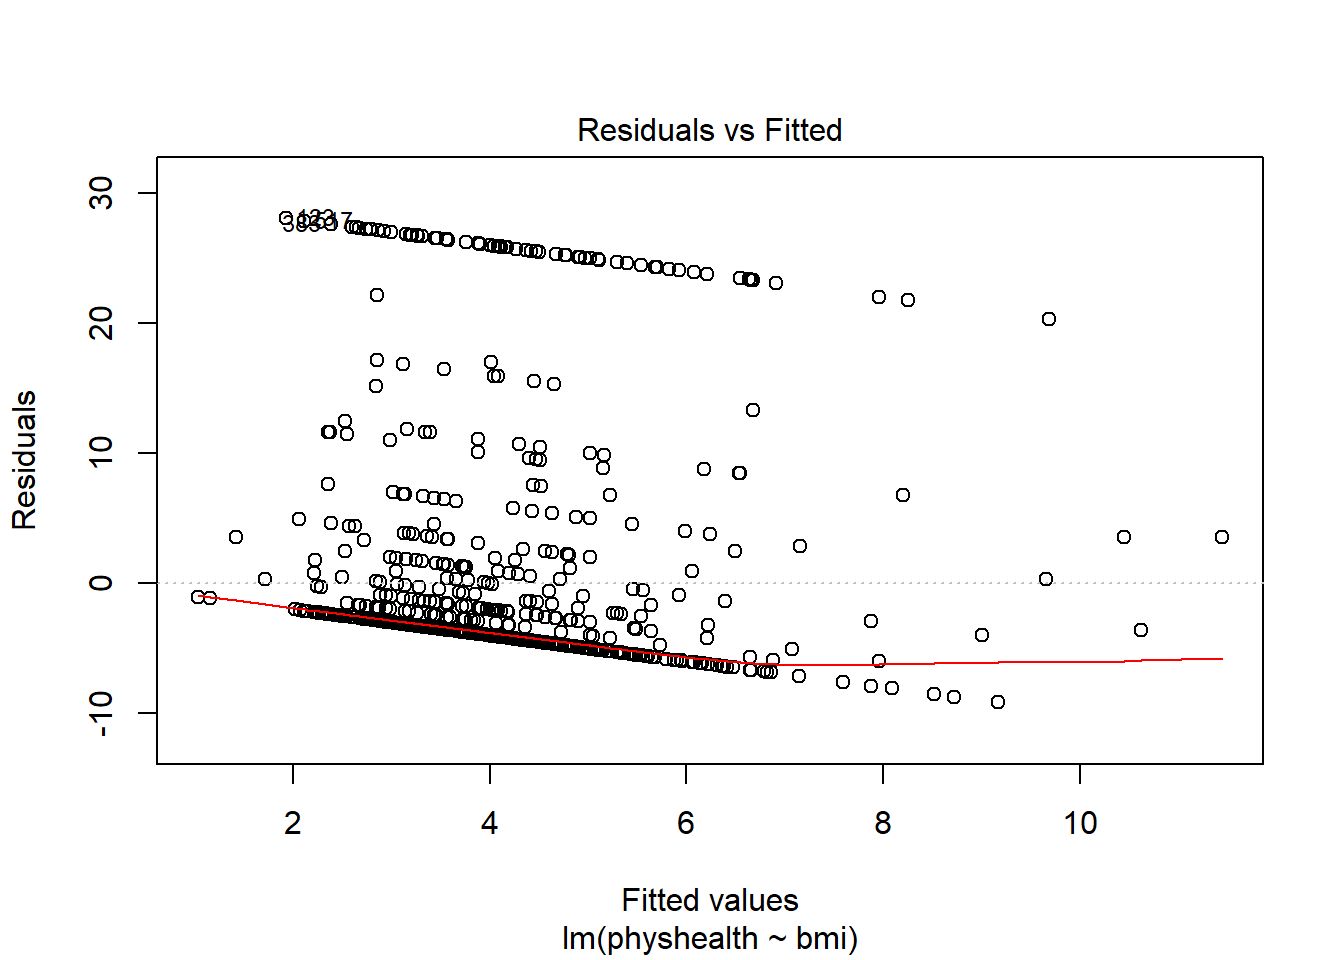
\includegraphics{bookdown-demo_files/figure-latex/chapter2_first_resid_plot_model_A-1.pdf}

This is a plot of residuals vs.~fitted values. The goal here is for this
plot to look like a random scatter of points, perhaps like a ``fuzzy
football'', and that's \textbf{not} what we have. Why?

If you prefer, here's a \texttt{ggplot2} version of a similar plot, now
looking at standardized residuals instead of raw residuals, and adding a
loess smooth and a linear fit to the result.

\begin{Shaded}
\begin{Highlighting}[]
\KeywordTok{ggplot}\NormalTok{(}\KeywordTok{augment}\NormalTok{(model_A), }\KeywordTok{aes}\NormalTok{(}\DataTypeTok{x =}\NormalTok{ .fitted, }\DataTypeTok{y =}\NormalTok{ .std.resid)) }\OperatorTok{+}
\StringTok{    }\KeywordTok{geom_point}\NormalTok{() }\OperatorTok{+}
\StringTok{    }\KeywordTok{geom_smooth}\NormalTok{(}\DataTypeTok{method =} \StringTok{"lm"}\NormalTok{, }\DataTypeTok{se =} \OtherTok{FALSE}\NormalTok{, }\DataTypeTok{col =} \StringTok{"red"}\NormalTok{, }\DataTypeTok{linetype =} \StringTok{"dashed"}\NormalTok{) }\OperatorTok{+}
\StringTok{    }\KeywordTok{geom_smooth}\NormalTok{(}\DataTypeTok{method =} \StringTok{"loess"}\NormalTok{, }\DataTypeTok{se =} \OtherTok{FALSE}\NormalTok{, }\DataTypeTok{col =} \StringTok{"navy"}\NormalTok{) }\OperatorTok{+}
\StringTok{    }\KeywordTok{theme_bw}\NormalTok{()}
\end{Highlighting}
\end{Shaded}

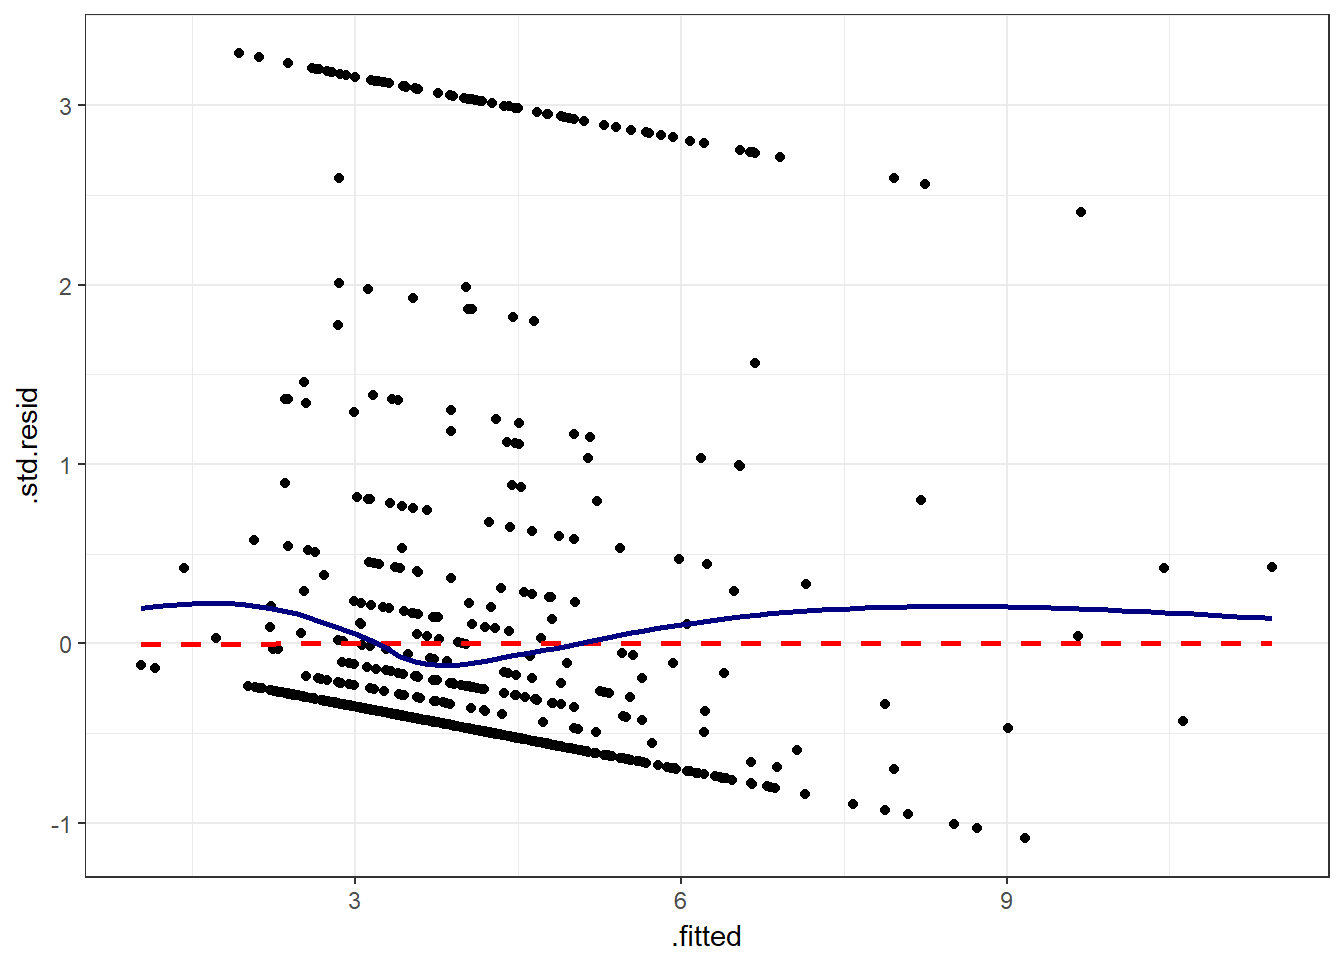
\includegraphics{bookdown-demo_files/figure-latex/chapter2_ggplot_first_resid_plot_model_A-1.pdf}

The problem we're having here becomes, I think, a little more obvious if
we look at what we're predicting. Does \texttt{physhealth} look like a
good candidate for a linear model?

\begin{Shaded}
\begin{Highlighting}[]
\KeywordTok{ggplot}\NormalTok{(smartcle2, }\KeywordTok{aes}\NormalTok{(}\DataTypeTok{x =}\NormalTok{ physhealth)) }\OperatorTok{+}
\KeywordTok{geom_histogram}\NormalTok{(}\DataTypeTok{bins =} \DecValTok{30}\NormalTok{, }\DataTypeTok{fill =} \StringTok{"dodgerblue"}\NormalTok{, }\DataTypeTok{color =} \StringTok{"royalblue"}\NormalTok{)}
\end{Highlighting}
\end{Shaded}

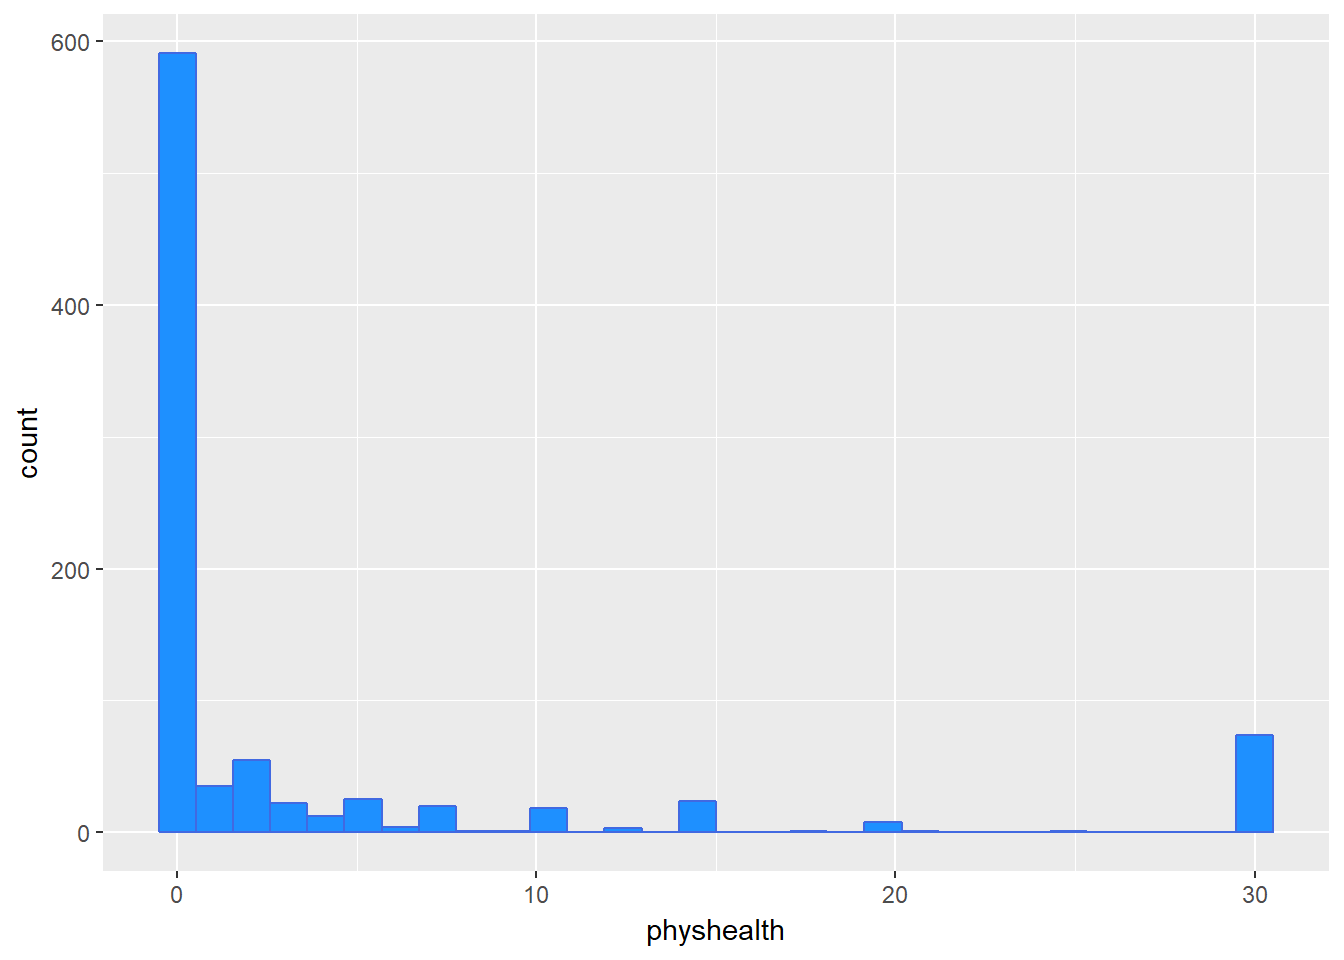
\includegraphics{bookdown-demo_files/figure-latex/histogram_of_physhealth_smartcle2-1.pdf}

\begin{Shaded}
\begin{Highlighting}[]
\NormalTok{smartcle2 }\OperatorTok\StringTok{ }\KeywordTok{count}\NormalTok{(physhealth }\OperatorTok{==}\StringTok{ }\DecValTok{0}\NormalTok{, physhealth }\OperatorTok{==}\StringTok{ }\DecValTok{30}\NormalTok{)}
\end{Highlighting}
\end{Shaded}

\begin{verbatim}
# A tibble: 3 x 3
  `physhealth == 0` `physhealth == 30`     n
  <lgl>             <lgl>              <int>
1 F                 F                    231
2 F                 T                     74
3 T                 F                    591
\end{verbatim}

No matter what model we fit, if we are predicting \texttt{physhealth},
and most of the data are values of 0 and 30, we have limited variation
in our outcome, and so our linear model will be somewhat questionable
just on that basis.

A normal Q-Q plot of the standardized residuals for our
\texttt{model\_A} shows this problem, too.

\begin{Shaded}
\begin{Highlighting}[]
\KeywordTok{plot}\NormalTok{(model_A, }\DataTypeTok{which =} \DecValTok{2}\NormalTok{)}
\end{Highlighting}
\end{Shaded}

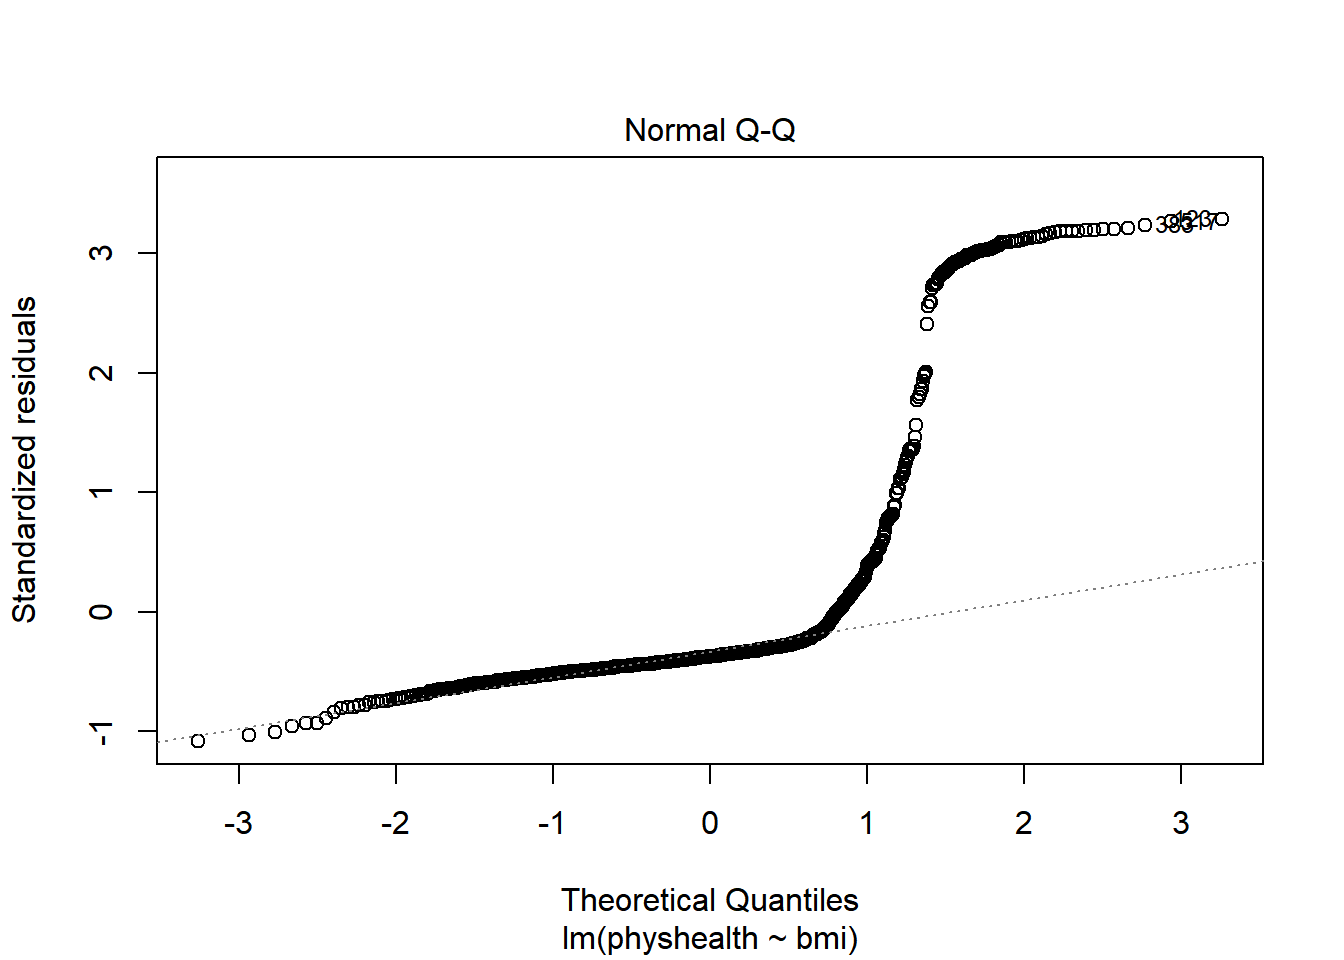
\includegraphics{bookdown-demo_files/figure-latex/chapter2_second_resid_plot_model_A-1.pdf}

We're going to need a method to deal with this sort of outcome, that has
both a floor and a ceiling. We'll get there eventually, but linear
regression alone doesn't look promising.

All right, so that didn't go anywhere great. Let's try again, with a new
outcome.

\section{A New Small Study}\label{a-new-small-study}

We'll begin by investigating the problem of predicting \texttt{bmi}, at
first with just three regression inputs: \texttt{sex}, \texttt{exerany}
and \texttt{sleephrs}, in our new \texttt{smartcle2} data set.

\begin{itemize}
\tightlist
\item
  The outcome of interest is \texttt{bmi}.
\item
  Inputs to the regression model are:

  \begin{itemize}
  \tightlist
  \item
    \texttt{female} = 1 if the subject is female, and 0 if they are male
  \item
    \texttt{exerany} = 1 if the subject exercised in the past 30 days,
    and 0 if they didn't
  \item
    \texttt{sleephrs} = hours slept in a typical 24-hour period (treated
    as quantitative)
  \end{itemize}
\end{itemize}

\subsection{Counting as exploratory data
analysis}\label{counting-as-exploratory-data-analysis}

Counting things can be amazingly useful.

\subsubsection{How many respondents had exercised in the past 30 days?
Did this vary by
sex?}\label{how-many-respondents-had-exercised-in-the-past-30-days-did-this-vary-by-sex}

\begin{Shaded}
\begin{Highlighting}[]
\NormalTok{smartcle2 }\OperatorTok\StringTok{ }\KeywordTok{count}\NormalTok{(female, exerany) }\OperatorTok\StringTok{ }\KeywordTok{mutate}\NormalTok{(}\DataTypeTok{percent =} \DecValTok{100}\OperatorTok{*}\NormalTok{n }\OperatorTok{/}\StringTok{ }\KeywordTok{sum}\NormalTok{(n))}
\end{Highlighting}
\end{Shaded}

\begin{verbatim}
# A tibble: 4 x 4
  female exerany     n percent
   <int>   <int> <int>   <dbl>
1      0       0    64    7.14
2      0       1   308   34.4 
3      1       0   145   16.2 
4      1       1   379   42.3 
\end{verbatim}

so we know now that 42.3\% of the subjects in our data were women who
exercised. Suppose that instead we want to find the percentage of
exercisers within each sex\ldots{}

\begin{Shaded}
\begin{Highlighting}[]
\NormalTok{smartcle2 }\OperatorTok
\StringTok{    }\KeywordTok{count}\NormalTok{(female, exerany) }\OperatorTok
\StringTok{    }\KeywordTok{group_by}\NormalTok{(female) }\OperatorTok
\StringTok{    }\KeywordTok{mutate}\NormalTok{(}\DataTypeTok{prob =} \DecValTok{100}\OperatorTok{*}\NormalTok{n }\OperatorTok{/}\StringTok{ }\KeywordTok{sum}\NormalTok{(n)) }
\end{Highlighting}
\end{Shaded}

\begin{verbatim}
# A tibble: 4 x 4
# Groups: female [2]
  female exerany     n  prob
   <int>   <int> <int> <dbl>
1      0       0    64  17.2
2      0       1   308  82.8
3      1       0   145  27.7
4      1       1   379  72.3
\end{verbatim}

and now we know that 82.8\% of the males exercised at least once in the
last 30 days, as compared to 72.3\% of the females.

\subsubsection{\texorpdfstring{What's the distribution of
\texttt{sleephrs}?}{What's the distribution of sleephrs?}}\label{whats-the-distribution-of-sleephrs}

We can count quantitative variables with discrete sets of possible
values, like \texttt{sleephrs}, which is captured as an integer (that
must fall between 0 and 24.)

\begin{Shaded}
\begin{Highlighting}[]
\NormalTok{smartcle2 }\OperatorTok\StringTok{ }\KeywordTok{count}\NormalTok{(sleephrs)}
\end{Highlighting}
\end{Shaded}

\begin{verbatim}
# A tibble: 14 x 2
   sleephrs     n
      <int> <int>
 1        1     5
 2        2     1
 3        3     6
 4        4    20
 5        5    63
 6        6   192
 7        7   276
 8        8   266
 9        9    38
10       10    22
11       11     2
12       12     2
13       16     2
14       20     1
\end{verbatim}

Of course, a natural summary of a quantitative variable like this would
be graphical.

\begin{Shaded}
\begin{Highlighting}[]
\KeywordTok{ggplot}\NormalTok{(smartcle2, }\KeywordTok{aes}\NormalTok{(sleephrs)) }\OperatorTok{+}
\StringTok{    }\KeywordTok{geom_histogram}\NormalTok{(}\DataTypeTok{binwidth =} \DecValTok{1}\NormalTok{, }\DataTypeTok{fill =} \StringTok{"dodgerblue"}\NormalTok{, }\DataTypeTok{col =} \StringTok{"darkred"}\NormalTok{)}
\end{Highlighting}
\end{Shaded}

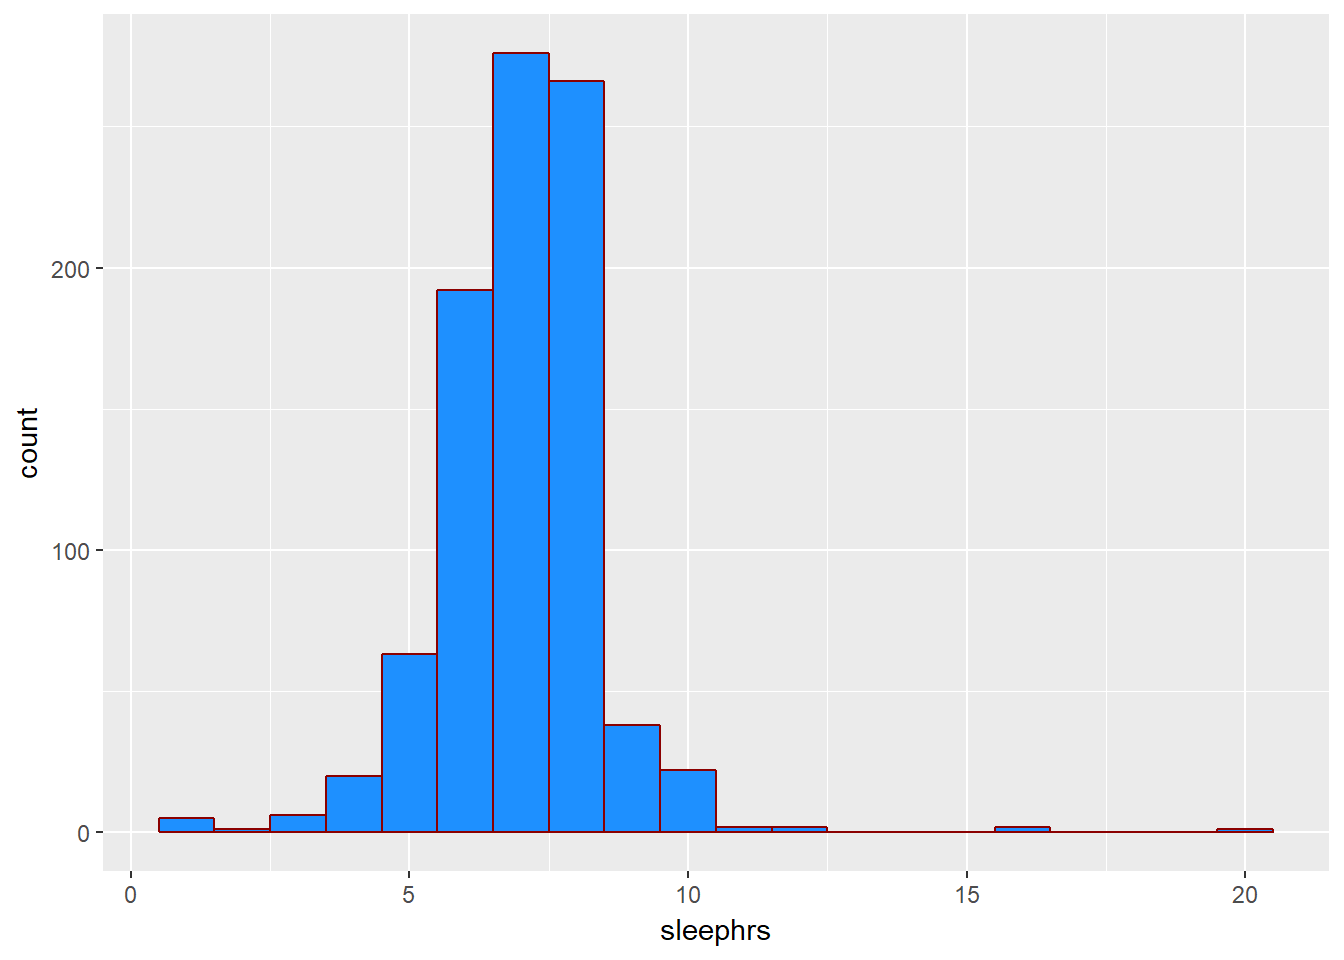
\includegraphics{bookdown-demo_files/figure-latex/c2_histogram_sleephrs_smartcle2-1.pdf}

\subsubsection{\texorpdfstring{What's the distribution of
\texttt{BMI}?}{What's the distribution of BMI?}}\label{whats-the-distribution-of-bmi}

\begin{Shaded}
\begin{Highlighting}[]
\KeywordTok{ggplot}\NormalTok{(smartcle2, }\KeywordTok{aes}\NormalTok{(bmi)) }\OperatorTok{+}
\StringTok{    }\KeywordTok{geom_histogram}\NormalTok{(}\DataTypeTok{bins =} \DecValTok{30}\NormalTok{, }\DataTypeTok{col =} \StringTok{"white"}\NormalTok{)}
\end{Highlighting}
\end{Shaded}

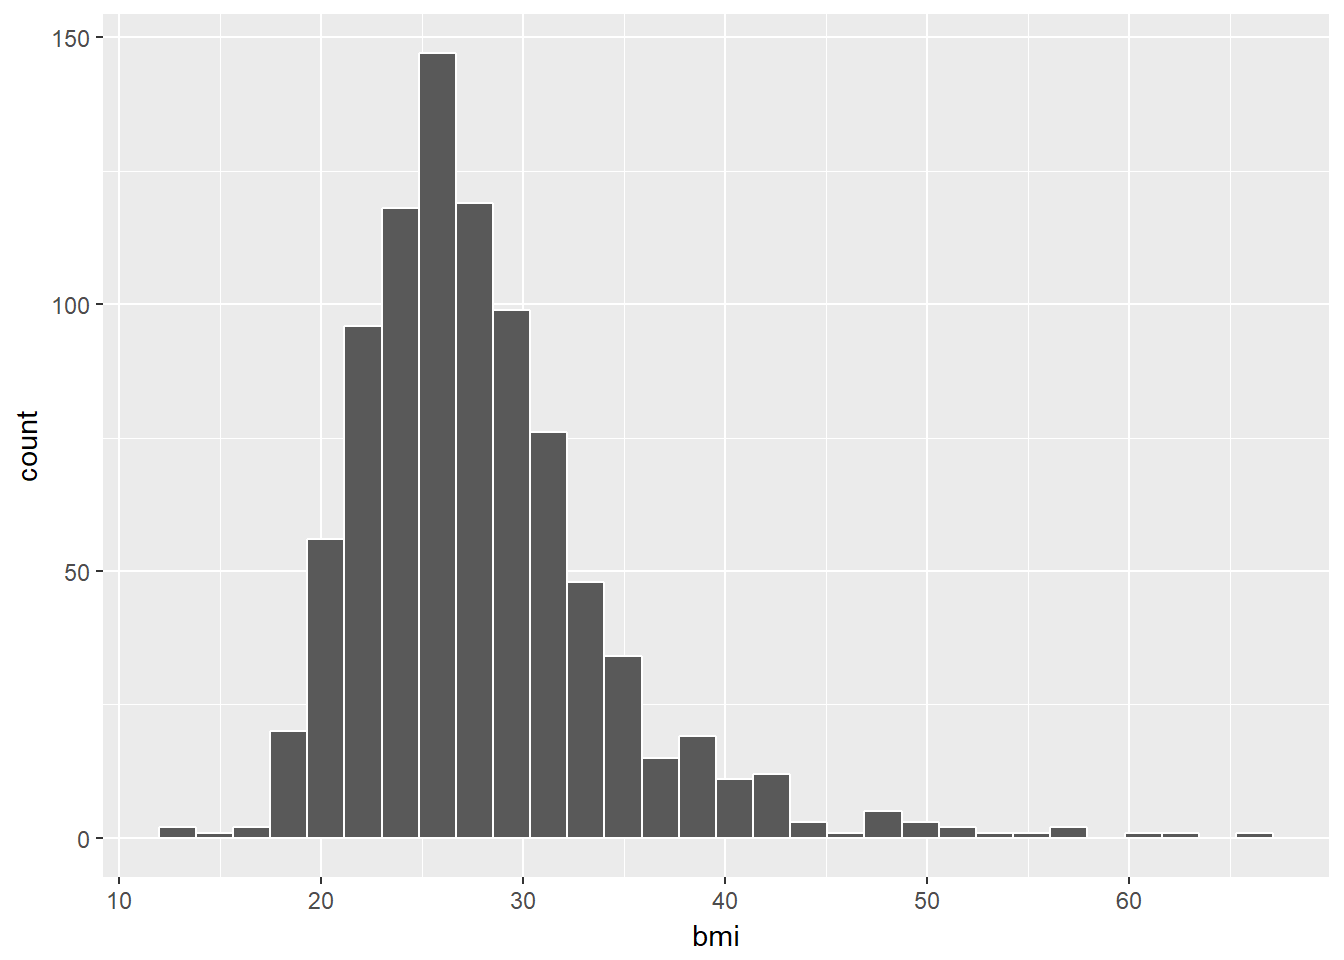
\includegraphics{bookdown-demo_files/figure-latex/c2_histogram_bmi_smartcle2-1.pdf}

\subsubsection{How many of the respondents have a BMI below
30?}\label{how-many-of-the-respondents-have-a-bmi-below-30}

\begin{Shaded}
\begin{Highlighting}[]
\NormalTok{smartcle2 }\OperatorTok\StringTok{ }\KeywordTok{count}\NormalTok{(bmi }\OperatorTok{<}\StringTok{ }\DecValTok{30}\NormalTok{) }\OperatorTok\StringTok{ }\KeywordTok{mutate}\NormalTok{(}\DataTypeTok{proportion =}\NormalTok{ n }\OperatorTok{/}\StringTok{ }\KeywordTok{sum}\NormalTok{(n))}
\end{Highlighting}
\end{Shaded}

\begin{verbatim}
# A tibble: 2 x 3
  `bmi < 30`     n proportion
  <lgl>      <int>      <dbl>
1 F            253      0.282
2 T            643      0.718
\end{verbatim}

\subsubsection{How many of the respondents who have a BMI \textless{} 30
exercised?}\label{how-many-of-the-respondents-who-have-a-bmi-30-exercised}

\begin{Shaded}
\begin{Highlighting}[]
\NormalTok{smartcle2 }\OperatorTok\StringTok{ }\KeywordTok{count}\NormalTok{(exerany, bmi }\OperatorTok{<}\StringTok{ }\DecValTok{30}\NormalTok{) }\OperatorTok
\StringTok{    }\KeywordTok{group_by}\NormalTok{(exerany) }\OperatorTok
\StringTok{    }\KeywordTok{mutate}\NormalTok{(}\DataTypeTok{percent =} \DecValTok{100}\OperatorTok{*}\NormalTok{n}\OperatorTok{/}\KeywordTok{sum}\NormalTok{(n))}
\end{Highlighting}
\end{Shaded}

\begin{verbatim}
# A tibble: 4 x 4
# Groups: exerany [2]
  exerany `bmi < 30`     n percent
    <int> <lgl>      <int>   <dbl>
1       0 F             88    42.1
2       0 T            121    57.9
3       1 F            165    24.0
4       1 T            522    76.0
\end{verbatim}

\subsubsection{Is obesity associated with sex, in these
data?}\label{is-obesity-associated-with-sex-in-these-data}

\begin{Shaded}
\begin{Highlighting}[]
\NormalTok{smartcle2 }\OperatorTok\StringTok{ }\KeywordTok{count}\NormalTok{(female, bmi }\OperatorTok{<}\StringTok{ }\DecValTok{30}\NormalTok{) }\OperatorTok
\StringTok{    }\KeywordTok{group_by}\NormalTok{(female) }\OperatorTok
\StringTok{    }\KeywordTok{mutate}\NormalTok{(}\DataTypeTok{percent =} \DecValTok{100}\OperatorTok{*}\NormalTok{n}\OperatorTok{/}\KeywordTok{sum}\NormalTok{(n))}
\end{Highlighting}
\end{Shaded}

\begin{verbatim}
# A tibble: 4 x 4
# Groups: female [2]
  female `bmi < 30`     n percent
   <int> <lgl>      <int>   <dbl>
1      0 F            105    28.2
2      0 T            267    71.8
3      1 F            148    28.2
4      1 T            376    71.8
\end{verbatim}

\subsubsection{\texorpdfstring{Comparing \texttt{sleephrs} summaries by
obesity
status}{Comparing sleephrs summaries by obesity status}}\label{comparing-sleephrs-summaries-by-obesity-status}

Can we compare the \texttt{sleephrs} means, medians and
75\textsuperscript{th} percentiles for respondents whose BMI is below 30
to the respondents whose BMI is not?

\begin{Shaded}
\begin{Highlighting}[]
\NormalTok{smartcle2 }\OperatorTok
\StringTok{    }\KeywordTok{group_by}\NormalTok{(bmi }\OperatorTok{<}\StringTok{ }\DecValTok{30}\NormalTok{) }\OperatorTok
\StringTok{    }\KeywordTok{summarize}\NormalTok{(}\KeywordTok{mean}\NormalTok{(sleephrs), }\KeywordTok{median}\NormalTok{(sleephrs), }
              \DataTypeTok{q75 =} \KeywordTok{quantile}\NormalTok{(sleephrs, }\FloatTok{0.75}\NormalTok{))}
\end{Highlighting}
\end{Shaded}

\begin{verbatim}
# A tibble: 2 x 4
  `bmi < 30` `mean(sleephrs)` `median(sleephrs)`   q75
  <lgl>                 <dbl>              <int> <dbl>
1 F                      6.93                  7  8.00
2 T                      7.06                  7  8.00
\end{verbatim}

\subsubsection{\texorpdfstring{The \texttt{skim} function within a
pipe}{The skim function within a pipe}}\label{the-skim-function-within-a-pipe}

The \textbf{skim} function works within pipes and with the other
\texttt{tidyverse} functions.

\begin{Shaded}
\begin{Highlighting}[]
\NormalTok{smartcle2 }\OperatorTok
\StringTok{    }\KeywordTok{group_by}\NormalTok{(exerany) }\OperatorTok
\StringTok{    }\KeywordTok{skim}\NormalTok{(bmi, sleephrs)}
\end{Highlighting}
\end{Shaded}

\begin{verbatim}
Skim summary statistics
 n obs: 896 
 n variables: 10 
 group variables: exerany 

Variable type: integer 
 exerany variable missing complete   n mean   sd p0 p25 median p75 p100
       0 sleephrs       0      209 209 7    1.85  1   6      7   8   20
       1 sleephrs       0      687 687 7.03 1.34  1   6      7   8   16

Variable type: numeric 
 exerany variable missing complete   n  mean   sd    p0   p25 median   p75
       0      bmi       0      209 209 29.57 7.46 18    24.11  28.49 33.13
       1      bmi       0      687 687 27.35 5.84 12.71 23.7   26.52 29.81
  p100
 66.06
 60.95
\end{verbatim}

\subsubsection{\texorpdfstring{The usual \texttt{summary} for a data
frame}{The usual summary for a data frame}}\label{the-usual-summary-for-a-data-frame}

Of course, we can use the usual \texttt{summary} to get some basic
information about the data, too.

\begin{Shaded}
\begin{Highlighting}[]
\KeywordTok{summary}\NormalTok{(smartcle2)}
\end{Highlighting}
\end{Shaded}

\begin{verbatim}
     SEQNO             physhealth      menthealth           genhealth  
 Min.   :2.016e+09   Min.   : 0.00   Min.   : 0.000   1_Excellent:155  
 1st Qu.:2.016e+09   1st Qu.: 0.00   1st Qu.: 0.000   2_VeryGood :306  
 Median :2.016e+09   Median : 0.00   Median : 0.000   3_Good     :295  
 Mean   :2.016e+09   Mean   : 3.99   Mean   : 2.693   4_Fair     :102  
 3rd Qu.:2.016e+09   3rd Qu.: 2.00   3rd Qu.: 2.000   5_Poor     : 38  
 Max.   :2.016e+09   Max.   :30.00   Max.   :30.000                    
      bmi            female         internet30        exerany      
 Min.   :12.71   Min.   :0.0000   Min.   :0.0000   Min.   :0.0000  
 1st Qu.:23.70   1st Qu.:0.0000   1st Qu.:1.0000   1st Qu.:1.0000  
 Median :26.80   Median :1.0000   Median :1.0000   Median :1.0000  
 Mean   :27.87   Mean   :0.5848   Mean   :0.8147   Mean   :0.7667  
 3rd Qu.:30.53   3rd Qu.:1.0000   3rd Qu.:1.0000   3rd Qu.:1.0000  
 Max.   :66.06   Max.   :1.0000   Max.   :1.0000   Max.   :1.0000  
    sleephrs         alcdays      
 Min.   : 1.000   Min.   : 0.000  
 1st Qu.: 6.000   1st Qu.: 0.000  
 Median : 7.000   Median : 1.000  
 Mean   : 7.022   Mean   : 4.834  
 3rd Qu.: 8.000   3rd Qu.: 5.000  
 Max.   :20.000   Max.   :30.000  
\end{verbatim}

\subsubsection{\texorpdfstring{The \texttt{describe} function in
\texttt{Hmisc}}{The describe function in Hmisc}}\label{the-describe-function-in-hmisc}

Or we can use the \texttt{describe} function from the \texttt{Hmisc}
package.

\begin{Shaded}
\begin{Highlighting}[]
\NormalTok{Hmisc}\OperatorTok{::}\KeywordTok{describe}\NormalTok{(smartcle2)}
\end{Highlighting}
\end{Shaded}

\begin{verbatim}
smartcle2 

 10  Variables      896  Observations
---------------------------------------------------------------------------
SEQNO 
        n   missing  distinct      Info      Mean       Gmd       .05 
      896         0       896         1 2.016e+09     345.7 2.016e+09 
      .10       .25       .50       .75       .90       .95 
2.016e+09 2.016e+09 2.016e+09 2.016e+09 2.016e+09 2.016e+09 

lowest : 2016000001 2016000002 2016000003 2016000004 2016000005
highest: 2016001031 2016001032 2016001033 2016001034 2016001036
---------------------------------------------------------------------------
physhealth 
       n  missing distinct     Info     Mean      Gmd      .05      .10 
     896        0       19    0.712     3.99    6.664        0        0 
     .25      .50      .75      .90      .95 
       0        0        2       15       30 
                                                                      
Value          0     1     2     3     4     5     6     7     8     9
Frequency    591    35    55    22    12    25     4    20     1     1
Proportion 0.660 0.039 0.061 0.025 0.013 0.028 0.004 0.022 0.001 0.001
                                                                
Value         10    12    14    15    18    20    21    25    30
Frequency     18     3    10    14     1     8     1     1    74
Proportion 0.020 0.003 0.011 0.016 0.001 0.009 0.001 0.001 0.083
---------------------------------------------------------------------------
menthealth 
       n  missing distinct     Info     Mean      Gmd      .05      .10 
     896        0       17    0.645    2.693    4.652        0        0 
     .25      .50      .75      .90      .95 
       0        0        2        8       20 
                                                                      
Value          0     1     2     3     4     5     6     7     8    10
Frequency    634    25    56    27    15    30     4    13     4    18
Proportion 0.708 0.028 0.062 0.030 0.017 0.033 0.004 0.015 0.004 0.020
                                                    
Value         14    15    18    20    23    29    30
Frequency      2    20     1     9     1     1    36
Proportion 0.002 0.022 0.001 0.010 0.001 0.001 0.040
---------------------------------------------------------------------------
genhealth 
       n  missing distinct 
     896        0        5 
                                                                      
Value      1_Excellent  2_VeryGood      3_Good      4_Fair      5_Poor
Frequency          155         306         295         102          38
Proportion       0.173       0.342       0.329       0.114       0.042
---------------------------------------------------------------------------
bmi 
       n  missing distinct     Info     Mean      Gmd      .05      .10 
     896        0      467        1    27.87    6.572    20.06    21.23 
     .25      .50      .75      .90      .95 
   23.70    26.80    30.53    35.36    39.30 

lowest : 12.71 13.34 14.72 16.22 17.30, highest: 56.89 57.04 60.95 61.84 66.06
---------------------------------------------------------------------------
female 
       n  missing distinct     Info      Sum     Mean      Gmd 
     896        0        2    0.728      524   0.5848   0.4862 

---------------------------------------------------------------------------
internet30 
       n  missing distinct     Info      Sum     Mean      Gmd 
     896        0        2    0.453      730   0.8147   0.3022 

---------------------------------------------------------------------------
exerany 
       n  missing distinct     Info      Sum     Mean      Gmd 
     896        0        2    0.537      687   0.7667   0.3581 

---------------------------------------------------------------------------
sleephrs 
       n  missing distinct     Info     Mean      Gmd      .05      .10 
     896        0       14    0.934    7.022    1.477        5        5 
     .25      .50      .75      .90      .95 
       6        7        8        8        9 
                                                                      
Value          1     2     3     4     5     6     7     8     9    10
Frequency      5     1     6    20    63   192   276   266    38    22
Proportion 0.006 0.001 0.007 0.022 0.070 0.214 0.308 0.297 0.042 0.025
                                  
Value         11    12    16    20
Frequency      2     2     2     1
Proportion 0.002 0.002 0.002 0.001
---------------------------------------------------------------------------
alcdays 
       n  missing distinct     Info     Mean      Gmd      .05      .10 
     896        0       22    0.909    4.834    7.189        0        0 
     .25      .50      .75      .90      .95 
       0        1        5       17       30 

lowest :  0  1  2  3  4, highest: 25 26 27 28 30
---------------------------------------------------------------------------
\end{verbatim}

\section{\texorpdfstring{Predicting
\texttt{bmi}}{Predicting bmi}}\label{predicting-bmi}

\subsection{\texorpdfstring{Does \texttt{female} predict \texttt{bmi}
well?}{Does female predict bmi well?}}\label{does-female-predict-bmi-well}

\subsubsection{Graphical Assessment}\label{graphical-assessment}

\begin{Shaded}
\begin{Highlighting}[]
\KeywordTok{ggplot}\NormalTok{(smartcle2, }\KeywordTok{aes}\NormalTok{(}\DataTypeTok{x =}\NormalTok{ female, }\DataTypeTok{y =}\NormalTok{ bmi)) }\OperatorTok{+}
\StringTok{    }\KeywordTok{geom_point}\NormalTok{()}
\end{Highlighting}
\end{Shaded}

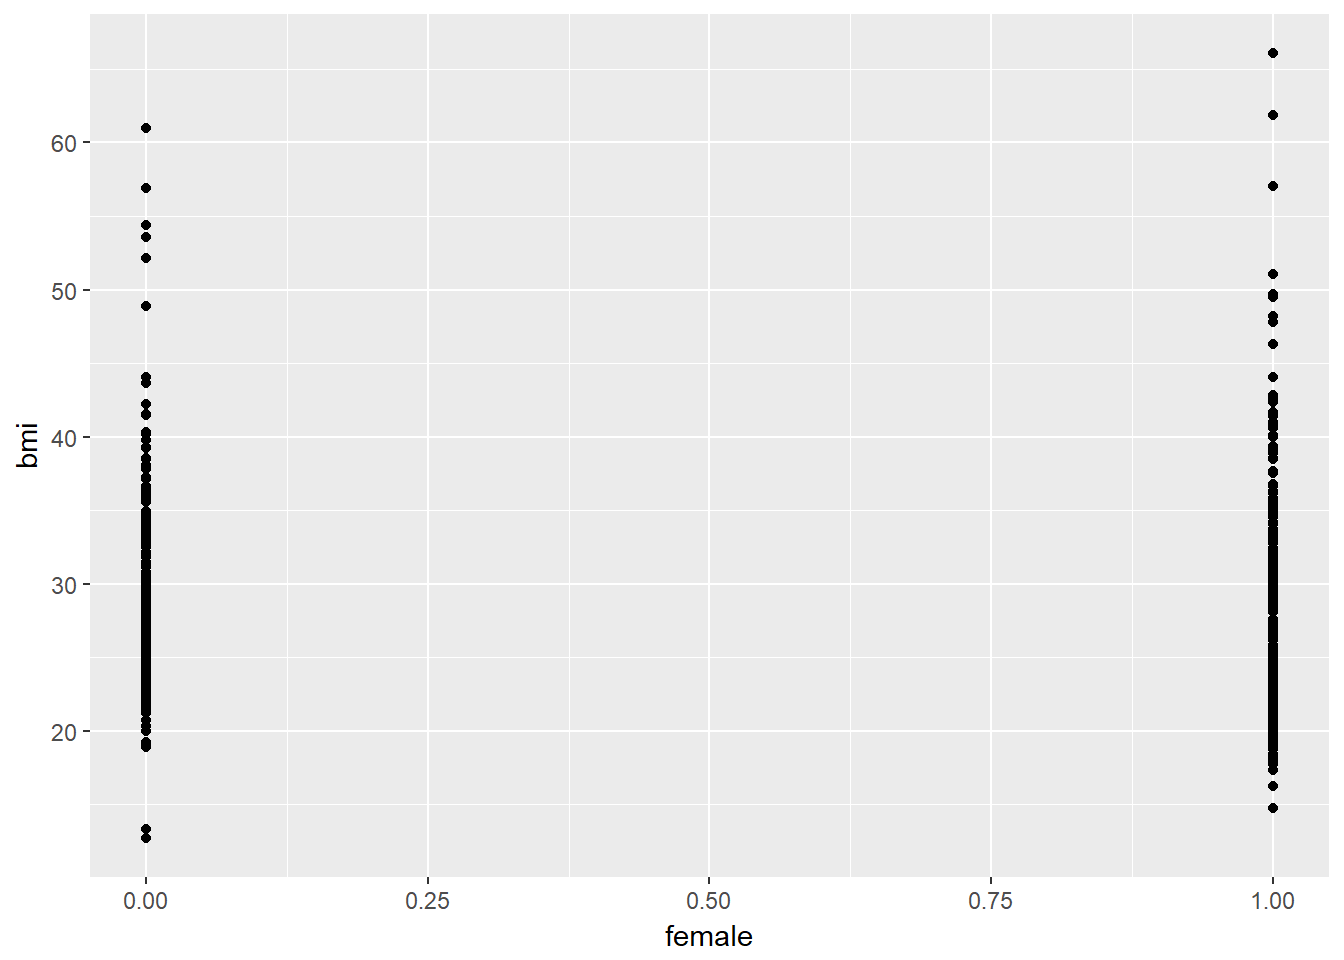
\includegraphics{bookdown-demo_files/figure-latex/c2_sex_bmi_plot1-1.pdf}

Not so helpful. We should probably specify that \texttt{female} is a
factor, and try another plotting approach.

\begin{Shaded}
\begin{Highlighting}[]
\KeywordTok{ggplot}\NormalTok{(smartcle2, }\KeywordTok{aes}\NormalTok{(}\DataTypeTok{x =} \KeywordTok{factor}\NormalTok{(female), }\DataTypeTok{y =}\NormalTok{ bmi)) }\OperatorTok{+}
\StringTok{    }\KeywordTok{geom_boxplot}\NormalTok{()}
\end{Highlighting}
\end{Shaded}

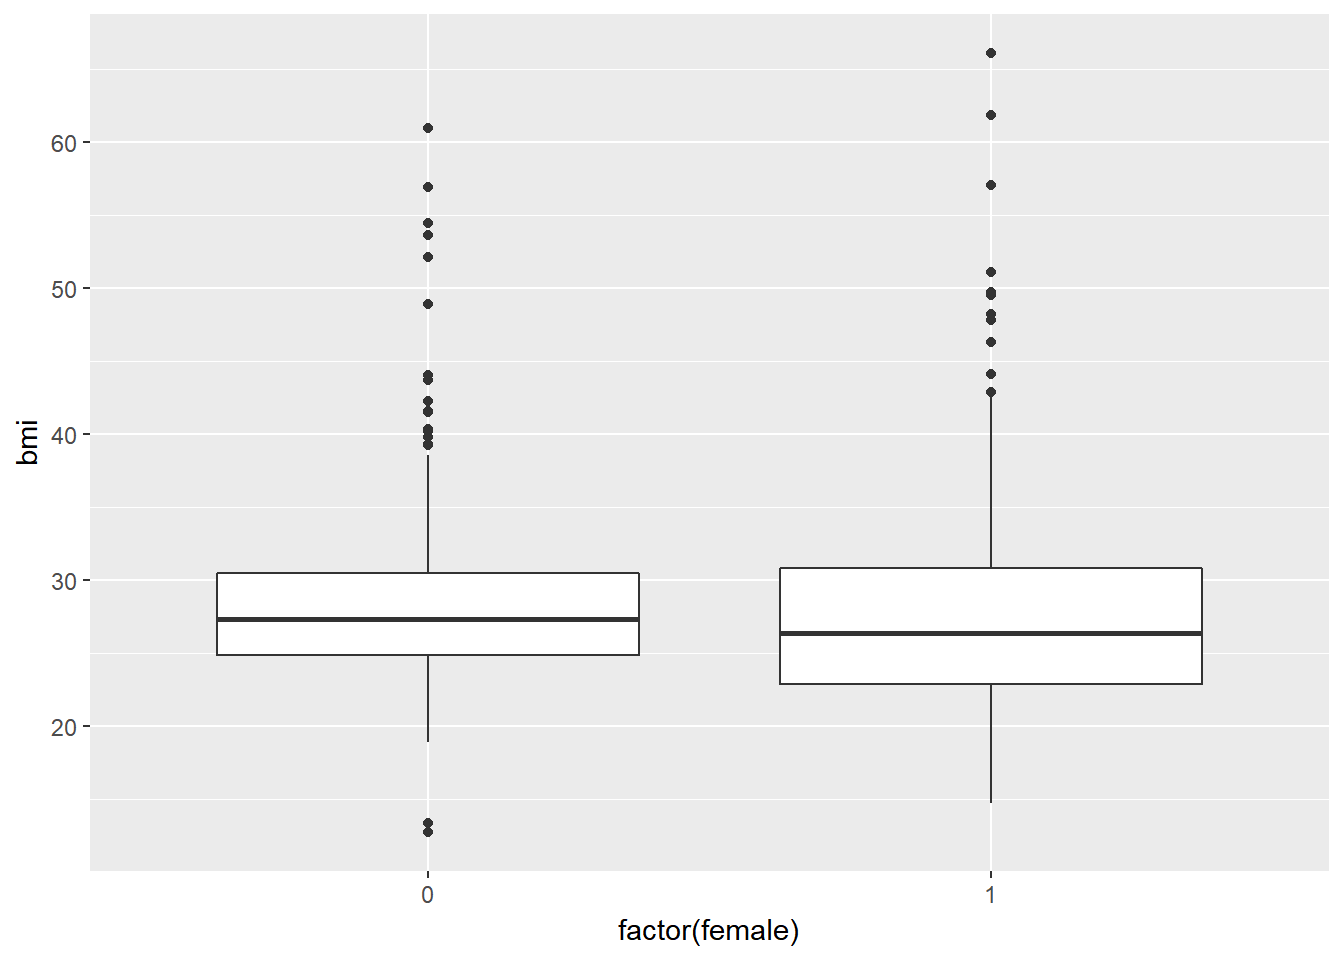
\includegraphics{bookdown-demo_files/figure-latex/c2_sex_bmi_plot2-1.pdf}

The median BMI looks a little higher for males. Let's see if a model
reflects that.

\subsubsection{\texorpdfstring{Model \texttt{c2\_m1}: A simple t-test
model}{Model c2\_m1: A simple t-test model}}\label{model-c2_m1-a-simple-t-test-model}

\begin{Shaded}
\begin{Highlighting}[]
\NormalTok{c2_m1 <-}\StringTok{ }\KeywordTok{lm}\NormalTok{(bmi }\OperatorTok{~}\StringTok{ }\NormalTok{female, }\DataTypeTok{data =}\NormalTok{ smartcle2)}
\NormalTok{c2_m1}
\end{Highlighting}
\end{Shaded}

\begin{verbatim}

Call:
lm(formula = bmi ~ female, data = smartcle2)

Coefficients:
(Intercept)       female  
    28.3600      -0.8457  
\end{verbatim}

\begin{Shaded}
\begin{Highlighting}[]
\KeywordTok{summary}\NormalTok{(c2_m1)}
\end{Highlighting}
\end{Shaded}

\begin{verbatim}

Call:
lm(formula = bmi ~ female, data = smartcle2)

Residuals:
    Min      1Q  Median      3Q     Max 
-15.650  -4.129  -1.080   2.727  38.546 

Coefficients:
            Estimate Std. Error t value Pr(>|t|)    
(Intercept)  28.3600     0.3274  86.613   <2e-16 ***
female       -0.8457     0.4282  -1.975   0.0485 *  
---
Signif. codes:  0 '***' 0.001 '**' 0.01 '*' 0.05 '.' 0.1 ' ' 1

Residual standard error: 6.315 on 894 degrees of freedom
Multiple R-squared:  0.004345,  Adjusted R-squared:  0.003231 
F-statistic: 3.902 on 1 and 894 DF,  p-value: 0.04855
\end{verbatim}

\begin{Shaded}
\begin{Highlighting}[]
\KeywordTok{confint}\NormalTok{(c2_m1)}
\end{Highlighting}
\end{Shaded}

\begin{verbatim}
                2.5 %      97.5 %
(Intercept) 27.717372 29.00262801
female      -1.686052 -0.00539878
\end{verbatim}

The model suggests, based on these 896 subjects, that

\begin{itemize}
\tightlist
\item
  our best prediction for males is BMI = 28.36 kg/m\textsuperscript{2},
  and
\item
  our best prediction for females is BMI = 28.36 - 0.85 = 27.51
  kg/m\textsuperscript{2}.
\item
  the mean difference between females and males is -0.85
  kg/m\textsuperscript{2} in BMI
\item
  a 95\% confidence (uncertainty) interval for that mean female - male
  difference in BMI ranges from -1.69 to -0.01
\item
  the model accounts for 0.4\% of the variation in BMI, so that knowing
  the respondent's sex does very little to reduce the size of the
  prediction errors as compared to an intercept only model that would
  predict the overall mean (regardless of sex) for all subjects.
\item
  the model makes some enormous errors, with one subject being predicted
  to have a BMI 38 points lower than his/her actual BMI.
\end{itemize}

Note that this simple regression model just gives us the t-test.

\begin{Shaded}
\begin{Highlighting}[]
\KeywordTok{t.test}\NormalTok{(bmi }\OperatorTok{~}\StringTok{ }\NormalTok{female, }\DataTypeTok{var.equal =} \OtherTok{TRUE}\NormalTok{, }\DataTypeTok{data =}\NormalTok{ smartcle2)}
\end{Highlighting}
\end{Shaded}

\begin{verbatim}

    Two Sample t-test

data:  bmi by female
t = 1.9752, df = 894, p-value = 0.04855
alternative hypothesis: true difference in means is not equal to 0
95 percent confidence interval:
 0.00539878 1.68605160
sample estimates:
mean in group 0 mean in group 1 
       28.36000        27.51427 
\end{verbatim}

\section{m2: Adding another predictor (two-way ANOVA without
interaction)}\label{m2-adding-another-predictor-two-way-anova-without-interaction}

When we add in the information about \texttt{exerany} to our original
model, we might first picture the data. We could look at separate
histograms,

\begin{Shaded}
\begin{Highlighting}[]
\KeywordTok{ggplot}\NormalTok{(smartcle2, }\KeywordTok{aes}\NormalTok{(}\DataTypeTok{x =}\NormalTok{ bmi)) }\OperatorTok{+}
\StringTok{    }\KeywordTok{geom_histogram}\NormalTok{(}\DataTypeTok{bins =} \DecValTok{30}\NormalTok{) }\OperatorTok{+}
\StringTok{    }\KeywordTok{facet_grid}\NormalTok{(female }\OperatorTok{~}\StringTok{ }\NormalTok{exerany, }\DataTypeTok{labeller =}\NormalTok{ label_both)}
\end{Highlighting}
\end{Shaded}

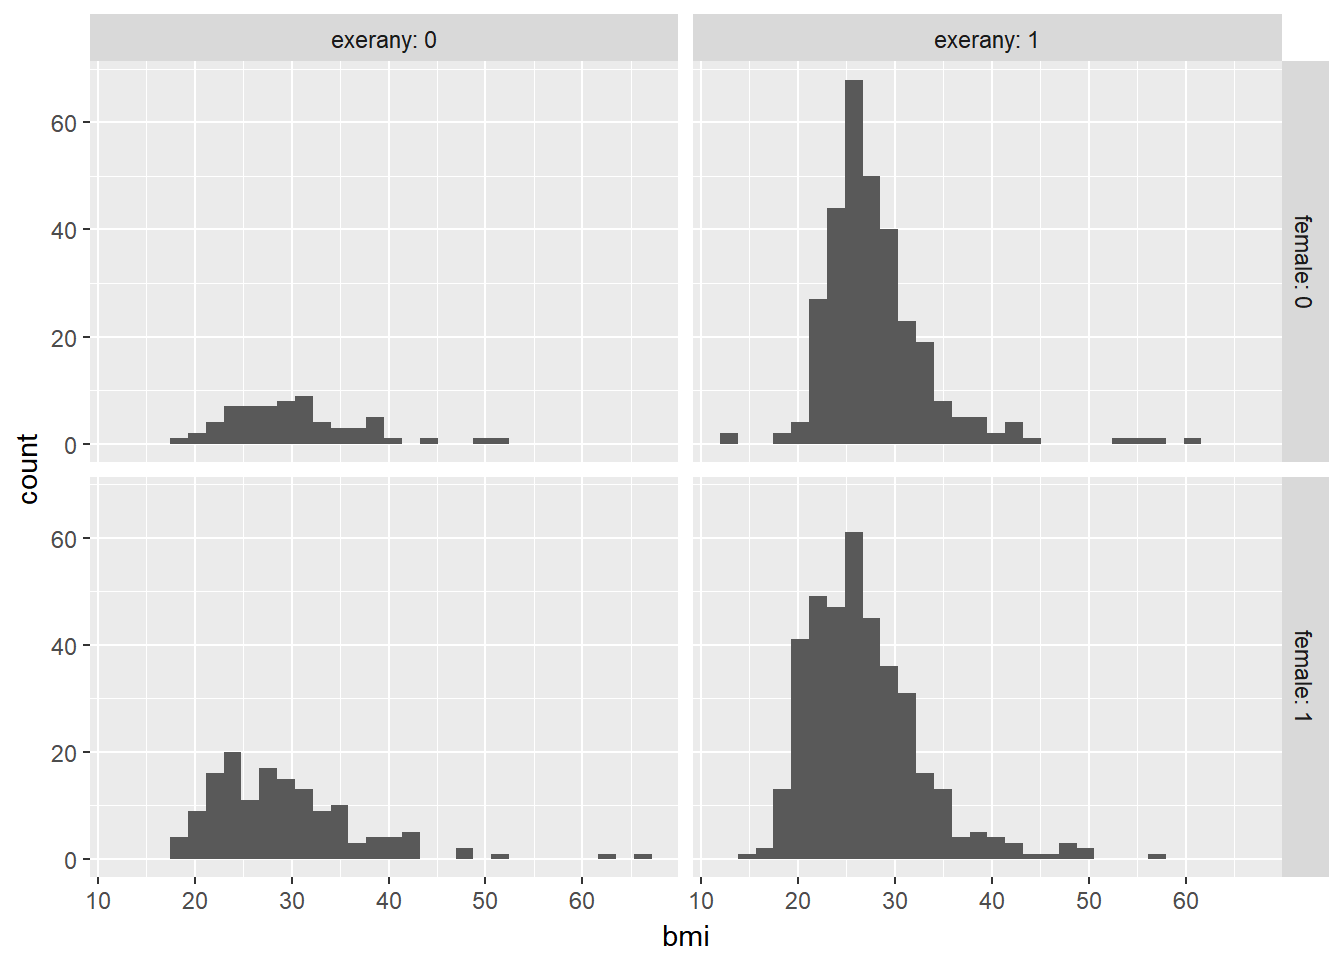
\includegraphics{bookdown-demo_files/figure-latex/c2_smartcle2_plot_bmi_hist_by_female_exerany-1.pdf}

or maybe boxplots?

\begin{Shaded}
\begin{Highlighting}[]
\KeywordTok{ggplot}\NormalTok{(smartcle2, }\KeywordTok{aes}\NormalTok{(}\DataTypeTok{x =} \KeywordTok{factor}\NormalTok{(female), }\DataTypeTok{y =}\NormalTok{ bmi)) }\OperatorTok{+}
\StringTok{    }\KeywordTok{geom_boxplot}\NormalTok{() }\OperatorTok{+}
\StringTok{    }\KeywordTok{facet_wrap}\NormalTok{(}\OperatorTok{~}\StringTok{ }\NormalTok{exerany, }\DataTypeTok{labeller =}\NormalTok{ label_both)}
\end{Highlighting}
\end{Shaded}

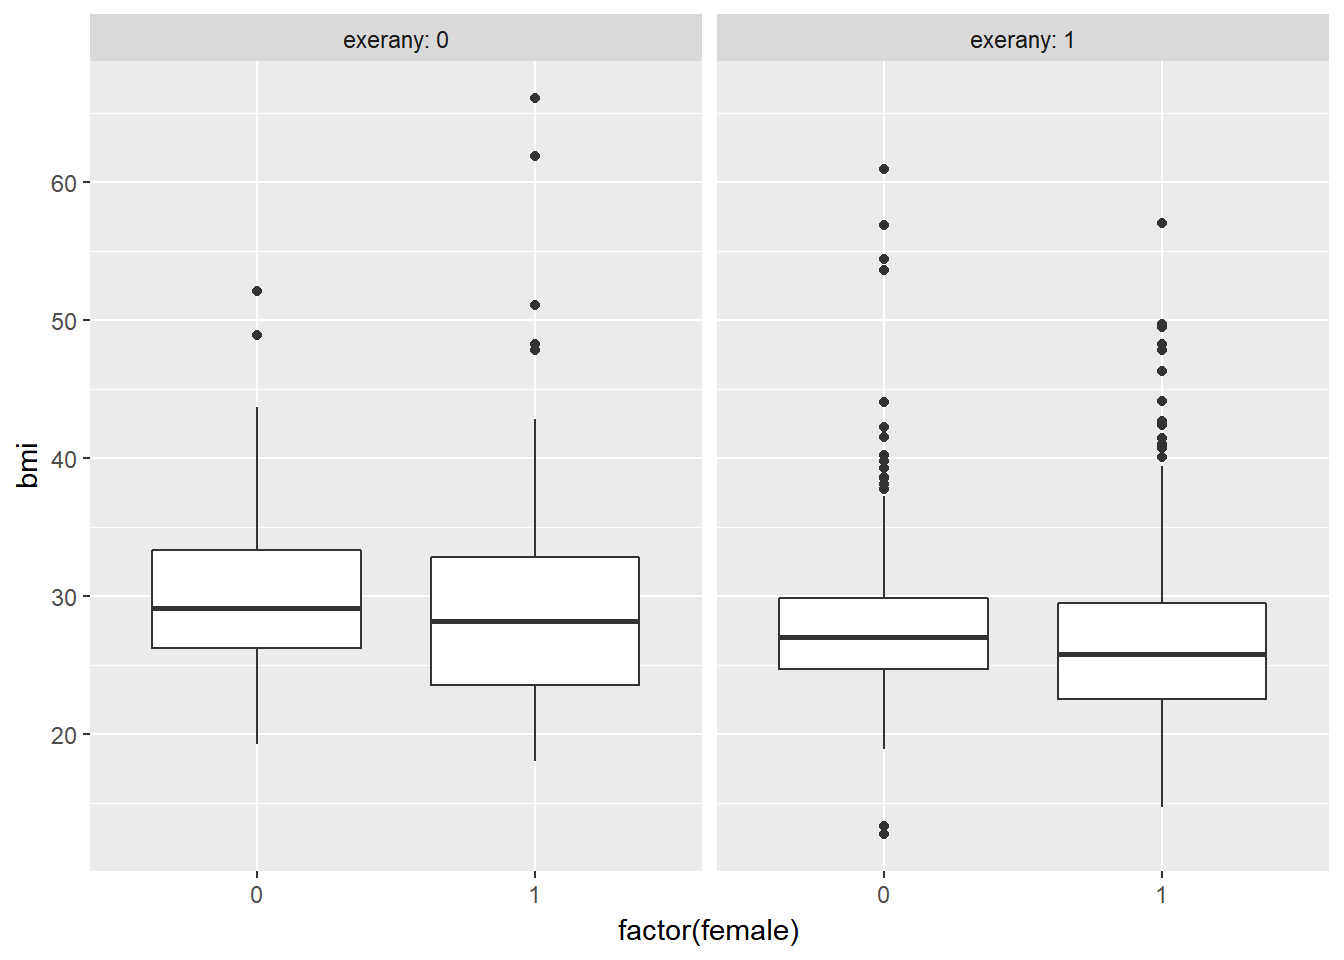
\includegraphics{bookdown-demo_files/figure-latex/c2_smartcle2_plot_bmi_box_by_female_exerany-1.pdf}

\begin{Shaded}
\begin{Highlighting}[]
\KeywordTok{ggplot}\NormalTok{(smartcle2, }\KeywordTok{aes}\NormalTok{(}\DataTypeTok{x =}\NormalTok{ female, }\DataTypeTok{y =}\NormalTok{ bmi))}\OperatorTok{+}
\StringTok{    }\KeywordTok{geom_point}\NormalTok{(}\DataTypeTok{size =} \DecValTok{3}\NormalTok{, }\DataTypeTok{alpha =} \FloatTok{0.2}\NormalTok{) }\OperatorTok{+}
\StringTok{    }\KeywordTok{theme_bw}\NormalTok{() }\OperatorTok{+}
\StringTok{    }\KeywordTok{facet_wrap}\NormalTok{(}\OperatorTok{~}\StringTok{ }\NormalTok{exerany, }\DataTypeTok{labeller =}\NormalTok{ label_both)}
\end{Highlighting}
\end{Shaded}

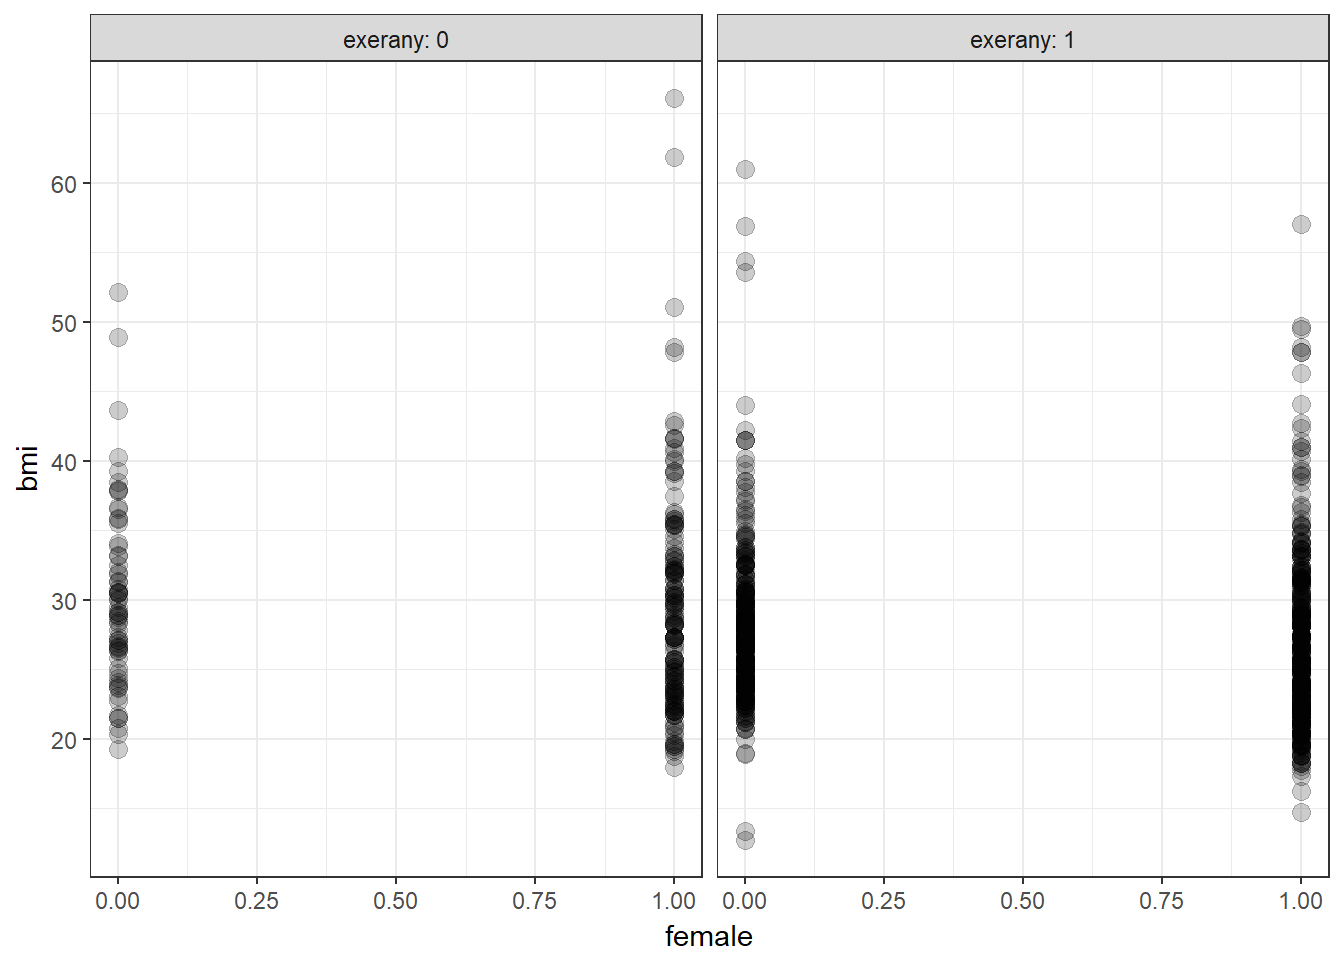
\includegraphics{bookdown-demo_files/figure-latex/c2_smartcle2_plot_bmi_points_by_female_exerany-1.pdf}

OK. Let's try fitting a model.

\begin{Shaded}
\begin{Highlighting}[]
\NormalTok{c2_m2 <-}\StringTok{ }\KeywordTok{lm}\NormalTok{(bmi }\OperatorTok{~}\StringTok{ }\NormalTok{female }\OperatorTok{+}\StringTok{ }\NormalTok{exerany, }\DataTypeTok{data =}\NormalTok{ smartcle2)}
\NormalTok{c2_m2}
\end{Highlighting}
\end{Shaded}

\begin{verbatim}

Call:
lm(formula = bmi ~ female + exerany, data = smartcle2)

Coefficients:
(Intercept)       female      exerany  
     30.334       -1.095       -2.384  
\end{verbatim}

This new model predicts only four predicted values:

\begin{itemize}
\tightlist
\item
  \texttt{bmi} = 30.334 if the subject is male and did not exercise (so
  \texttt{female} = 0 and \texttt{exerany} = 0)
\item
  \texttt{bmi} = 30.334 - 1.095 = 29.239 if the subject is female and
  did not exercise (\texttt{female} = 1 and \texttt{exerany} = 0)
\item
  \texttt{bmi} = 30.334 - 2.384 = 27.950 if the subject is male and
  exercised (so \texttt{female} = 0 and \texttt{exerany} = 1), and,
  finally
\item
  \texttt{bmi} = 30.334 - 1.095 - 2.384 = 26.855 if the subject is
  female and exercised (so both \texttt{female} and \texttt{exerany} =
  1).
\end{itemize}

For those who did not exercise, the model is:

\begin{itemize}
\tightlist
\item
  \texttt{bmi} = 30.334 - 1.095 \texttt{female}
\end{itemize}

and for those who did exercise, the model is:

\begin{itemize}
\tightlist
\item
  \texttt{bmi} = 27.95 - 1.095 \texttt{female}
\end{itemize}

Only the intercept of the \texttt{bmi-female} model changes depending on
\texttt{exerany}.

\begin{Shaded}
\begin{Highlighting}[]
\KeywordTok{summary}\NormalTok{(c2_m2)}
\end{Highlighting}
\end{Shaded}

\begin{verbatim}

Call:
lm(formula = bmi ~ female + exerany, data = smartcle2)

Residuals:
    Min      1Q  Median      3Q     Max 
-15.240  -4.091  -1.095   2.602  36.822 

Coefficients:
            Estimate Std. Error t value Pr(>|t|)    
(Intercept)  30.3335     0.5231   57.99  < 2e-16 ***
female       -1.0952     0.4262   -2.57   0.0103 *  
exerany      -2.3836     0.4965   -4.80 1.86e-06 ***
---
Signif. codes:  0 '***' 0.001 '**' 0.01 '*' 0.05 '.' 0.1 ' ' 1

Residual standard error: 6.239 on 893 degrees of freedom
Multiple R-squared:  0.02939,   Adjusted R-squared:  0.02722 
F-statistic: 13.52 on 2 and 893 DF,  p-value: 1.641e-06
\end{verbatim}

\begin{Shaded}
\begin{Highlighting}[]
\KeywordTok{confint}\NormalTok{(c2_m2)}
\end{Highlighting}
\end{Shaded}

\begin{verbatim}
                2.5 %     97.5 %
(Intercept) 29.306846 31.3602182
female      -1.931629 -0.2588299
exerany     -3.358156 -1.4090777
\end{verbatim}

The slopes of both \texttt{female} and \texttt{exerany} have confidence
intervals that are completely below zero, indicating that both
\texttt{female} sex and \texttt{exerany} appear to be associated with
reductions in \texttt{bmi}.

The R\textsuperscript{2} value suggests that just under 3\% of the
variation in \texttt{bmi} is accounted for by this ANOVA model.

In fact, this regression (on two binary indicator variables) is simply a
two-way ANOVA model without an interaction term.

\begin{Shaded}
\begin{Highlighting}[]
\KeywordTok{anova}\NormalTok{(c2_m2)}
\end{Highlighting}
\end{Shaded}

\begin{verbatim}
Analysis of Variance Table

Response: bmi
           Df Sum Sq Mean Sq F value    Pr(>F)    
female      1    156  155.61  3.9977   0.04586 *  
exerany     1    897  896.93 23.0435 1.856e-06 ***
Residuals 893  34759   38.92                      
---
Signif. codes:  0 '***' 0.001 '**' 0.01 '*' 0.05 '.' 0.1 ' ' 1
\end{verbatim}

\section{m3: Adding the interaction term (Two-way ANOVA with
interaction)}\label{m3-adding-the-interaction-term-two-way-anova-with-interaction}

Suppose we want to let the effect of \texttt{female} vary depending on
the \texttt{exerany} status. Then we need to incorporate an interaction
term in our model.

\begin{Shaded}
\begin{Highlighting}[]
\NormalTok{c2_m3 <-}\StringTok{ }\KeywordTok{lm}\NormalTok{(bmi }\OperatorTok{~}\StringTok{ }\NormalTok{female }\OperatorTok{*}\StringTok{ }\NormalTok{exerany, }\DataTypeTok{data =}\NormalTok{ smartcle2)}
\NormalTok{c2_m3}
\end{Highlighting}
\end{Shaded}

\begin{verbatim}

Call:
lm(formula = bmi ~ female * exerany, data = smartcle2)

Coefficients:
   (Intercept)          female         exerany  female:exerany  
       30.1359         -0.8104         -2.1450         -0.3592  
\end{verbatim}

So, for example, for a male who exercises, this model predicts

\begin{itemize}
\tightlist
\item
  \texttt{bmi} = 30.136 - 0.810 (0) - 2.145 (1) - 0.359 (0)(1) = 30.136
  - 2.145 = 27.991
\end{itemize}

And for a female who exercises, the model predicts

\begin{itemize}
\tightlist
\item
  \texttt{bmi} = 30.136 - 0.810 (1) - 2.145 (1) - 0.359 (1)(1) = 30.136
  - 0.810 - 2.145 - 0.359 = 26.822
\end{itemize}

For those who did not exercise, the model is:

\begin{itemize}
\tightlist
\item
  \texttt{bmi} = 30.136 - 0.81 \texttt{female}
\end{itemize}

But for those who did exercise, the model is:

\begin{itemize}
\tightlist
\item
  \texttt{bmi} = (30.136 - 2.145) + (-0.810 + (-0.359)) \texttt{female},
  or ,,,
\item
  \texttt{bmi} = 27.991 - 1.169 \texttt{female}
\end{itemize}

Now, both the slope and the intercept of the \texttt{bmi-female} model
change depending on \texttt{exerany}.

\begin{Shaded}
\begin{Highlighting}[]
\KeywordTok{summary}\NormalTok{(c2_m3)}
\end{Highlighting}
\end{Shaded}

\begin{verbatim}

Call:
lm(formula = bmi ~ female * exerany, data = smartcle2)

Residuals:
    Min      1Q  Median      3Q     Max 
-15.281  -4.101  -1.061   2.566  36.734 

Coefficients:
               Estimate Std. Error t value Pr(>|t|)    
(Intercept)     30.1359     0.7802  38.624   <2e-16 ***
female          -0.8104     0.9367  -0.865   0.3872    
exerany         -2.1450     0.8575  -2.501   0.0125 *  
female:exerany  -0.3592     1.0520  -0.341   0.7328    
---
Signif. codes:  0 '***' 0.001 '**' 0.01 '*' 0.05 '.' 0.1 ' ' 1

Residual standard error: 6.242 on 892 degrees of freedom
Multiple R-squared:  0.02952,   Adjusted R-squared:  0.02625 
F-statistic: 9.044 on 3 and 892 DF,  p-value: 6.669e-06
\end{verbatim}

\begin{Shaded}
\begin{Highlighting}[]
\KeywordTok{confint}\NormalTok{(c2_m3)}
\end{Highlighting}
\end{Shaded}

\begin{verbatim}
                   2.5 %     97.5 %
(Intercept)    28.604610 31.6672650
female         -2.648893  1.0280526
exerany        -3.827886 -0.4620407
female:exerany -2.423994  1.7055248
\end{verbatim}

In fact, this regression (on two binary indicator variables and a
product term) is simply a two-way ANOVA model with an interaction term.

\begin{Shaded}
\begin{Highlighting}[]
\KeywordTok{anova}\NormalTok{(c2_m3)}
\end{Highlighting}
\end{Shaded}

\begin{verbatim}
Analysis of Variance Table

Response: bmi
                Df Sum Sq Mean Sq F value    Pr(>F)    
female           1    156  155.61  3.9938   0.04597 *  
exerany          1    897  896.93 23.0207 1.878e-06 ***
female:exerany   1      5    4.54  0.1166   0.73283    
Residuals      892  34754   38.96                      
---
Signif. codes:  0 '***' 0.001 '**' 0.01 '*' 0.05 '.' 0.1 ' ' 1
\end{verbatim}

The interaction term doesn't change very much here. Its uncertainty
interval includes zero, and the overall model still accounts for just
under 3\% of the variation in \texttt{bmi}.

\section{\texorpdfstring{m4: Using \texttt{female} and \texttt{sleephrs}
in a model for
\texttt{bmi}}{m4: Using female and sleephrs in a model for bmi}}\label{m4-using-female-and-sleephrs-in-a-model-for-bmi}

\begin{Shaded}
\begin{Highlighting}[]
\KeywordTok{ggplot}\NormalTok{(smartcle2, }\KeywordTok{aes}\NormalTok{(}\DataTypeTok{x =}\NormalTok{ sleephrs, }\DataTypeTok{y =}\NormalTok{ bmi, }\DataTypeTok{color =} \KeywordTok{factor}\NormalTok{(female))) }\OperatorTok{+}
\StringTok{    }\KeywordTok{geom_point}\NormalTok{() }\OperatorTok{+}\StringTok{ }
\StringTok{    }\KeywordTok{guides}\NormalTok{(}\DataTypeTok{col =} \OtherTok{FALSE}\NormalTok{) }\OperatorTok{+}
\StringTok{    }\KeywordTok{geom_smooth}\NormalTok{(}\DataTypeTok{method =} \StringTok{"lm"}\NormalTok{, }\DataTypeTok{se =} \OtherTok{FALSE}\NormalTok{) }\OperatorTok{+}
\StringTok{    }\KeywordTok{facet_wrap}\NormalTok{(}\OperatorTok{~}\StringTok{ }\NormalTok{female, }\DataTypeTok{labeller =}\NormalTok{ label_both) }
\end{Highlighting}
\end{Shaded}

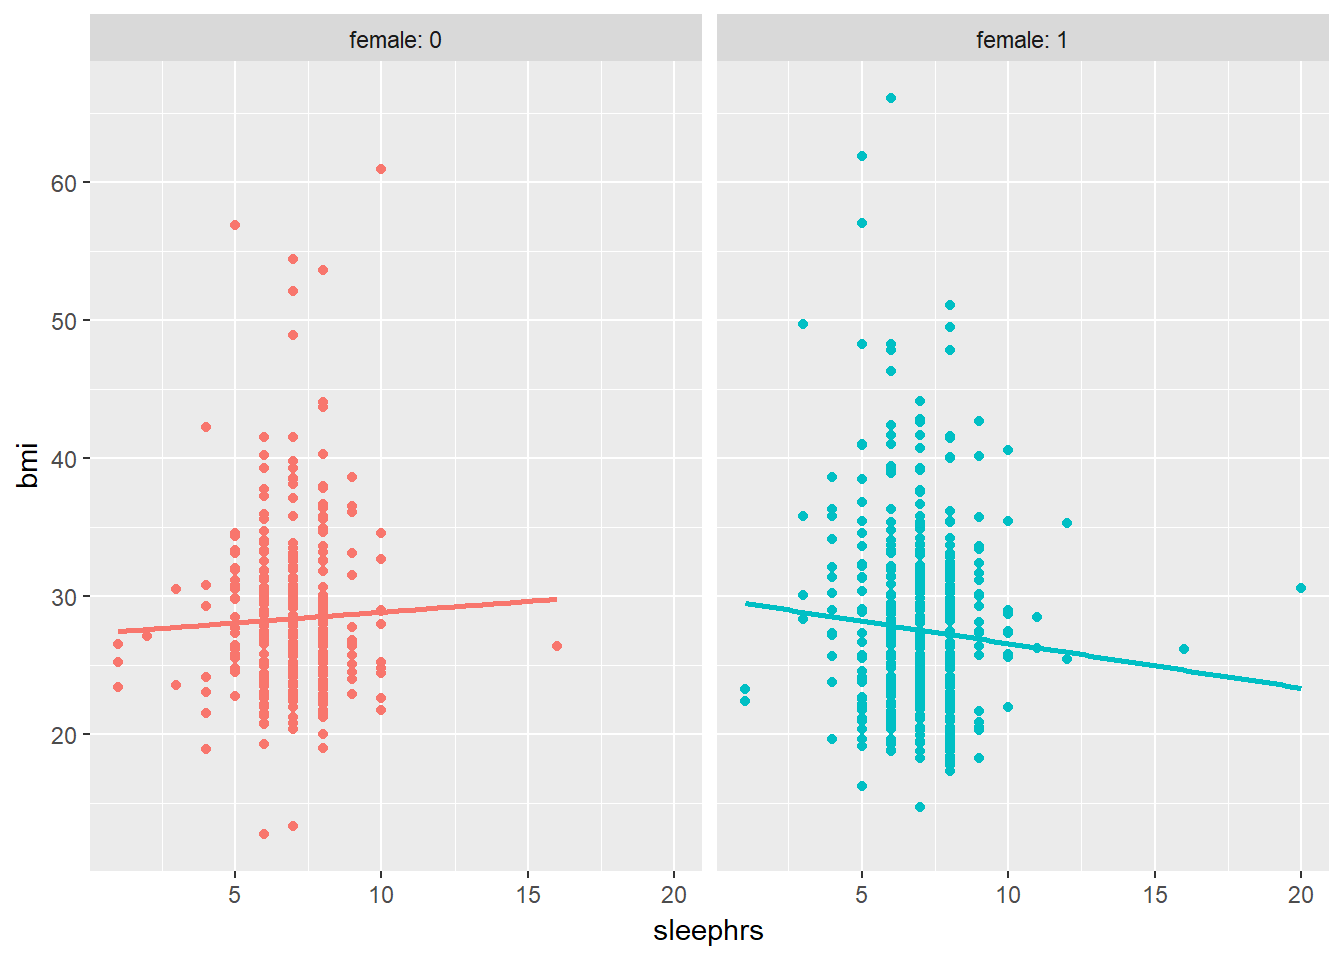
\includegraphics{bookdown-demo_files/figure-latex/graph_to_set_up_c2_m4-1.pdf}

Does the difference in slopes of \texttt{bmi} and \texttt{sleephrs} for
males and females appear to be substantial and important?

\begin{Shaded}
\begin{Highlighting}[]
\NormalTok{c2_m4 <-}\StringTok{ }\KeywordTok{lm}\NormalTok{(bmi }\OperatorTok{~}\StringTok{ }\NormalTok{female }\OperatorTok{*}\StringTok{ }\NormalTok{sleephrs, }\DataTypeTok{data =}\NormalTok{ smartcle2)}

\KeywordTok{summary}\NormalTok{(c2_m4)}
\end{Highlighting}
\end{Shaded}

\begin{verbatim}

Call:
lm(formula = bmi ~ female * sleephrs, data = smartcle2)

Residuals:
    Min      1Q  Median      3Q     Max 
-15.498  -4.179  -1.035   2.830  38.204 

Coefficients:
                Estimate Std. Error t value Pr(>|t|)    
(Intercept)      27.2661     1.6320  16.707   <2e-16 ***
female            2.5263     2.0975   1.204    0.229    
sleephrs          0.1569     0.2294   0.684    0.494    
female:sleephrs  -0.4797     0.2931  -1.636    0.102    
---
Signif. codes:  0 '***' 0.001 '**' 0.01 '*' 0.05 '.' 0.1 ' ' 1

Residual standard error: 6.31 on 892 degrees of freedom
Multiple R-squared:  0.008341,  Adjusted R-squared:  0.005006 
F-statistic: 2.501 on 3 and 892 DF,  p-value: 0.05818
\end{verbatim}

Does it seem as though the addition of \texttt{sleephrs} has improved
our model substantially over a model with \texttt{female} alone (which,
you recall, was \texttt{c2\_m1})?

Since the \texttt{c2\_m4} model contains the \texttt{c2\_m1} model's
predictors as a subset and the outcome is the same for each model, we
consider the models \emph{nested} and have some extra tools available to
compare them.

\begin{itemize}
\tightlist
\item
  I might start by looking at the basic summaries for each model.
\end{itemize}

\begin{Shaded}
\begin{Highlighting}[]
\KeywordTok{glance}\NormalTok{(c2_m4)}
\end{Highlighting}
\end{Shaded}

\begin{verbatim}
    r.squared adj.r.squared    sigma statistic    p.value df    logLik
1 0.008341404   0.005006229 6.309685   2.50104 0.05818038  4 -2919.873
       AIC      BIC deviance df.residual
1 5849.747 5873.736 35512.42         892
\end{verbatim}

\begin{Shaded}
\begin{Highlighting}[]
\KeywordTok{glance}\NormalTok{(c2_m1)}
\end{Highlighting}
\end{Shaded}

\begin{verbatim}
    r.squared adj.r.squared   sigma statistic    p.value df    logLik
1 0.004345169   0.003231461 6.31531  3.901534 0.04854928  2 -2921.675
      AIC      BIC deviance df.residual
1 5849.35 5863.744 35655.53         894
\end{verbatim}

\begin{itemize}
\tightlist
\item
  The R\textsuperscript{2} is twice as large for the model with
  \texttt{sleephrs}, but still very tiny.
\item
  The \emph{p} value for the global ANOVA test is actually less
  significant in \texttt{c2\_m4} than in \texttt{c2\_m1}.
\item
  Smaller AIC and smaller BIC statistics are more desirable. Here,
  there's little to choose from, but \texttt{c2\_m1} is a little better
  on each standard.
\item
  We might also consider a significance test by looking at an ANOVA
  model comparison. This is only appropriate because \texttt{c2\_m1} is
  nested in \texttt{c2\_m4}.
\end{itemize}

\begin{Shaded}
\begin{Highlighting}[]
\KeywordTok{anova}\NormalTok{(c2_m4, c2_m1)}
\end{Highlighting}
\end{Shaded}

\begin{verbatim}
Analysis of Variance Table

Model 1: bmi ~ female * sleephrs
Model 2: bmi ~ female
  Res.Df   RSS Df Sum of Sq      F Pr(>F)
1    892 35512                           
2    894 35656 -2   -143.11 1.7973 0.1663
\end{verbatim}

The addition of the \texttt{sleephrs} term picked up 143 in the sum of
squares column, at a cost of two degrees of freedom, yielding a \emph{p}
value of 0.166, suggesting that this isn't a significant improvement
over the model that just did a t-test on \texttt{female}.

\section{m5: What if we add more
variables?}\label{m5-what-if-we-add-more-variables}

We can boost our R\textsuperscript{2} a bit, to over 5\%, by adding in
two new variables, related to whether or not the subject (in the past 30
days) used the internet, and on how many days the subject drank
alcoholic beverages.

\begin{Shaded}
\begin{Highlighting}[]
\NormalTok{c2_m5 <-}\StringTok{ }\KeywordTok{lm}\NormalTok{(bmi }\OperatorTok{~}\StringTok{ }\NormalTok{female }\OperatorTok{+}\StringTok{ }\NormalTok{exerany }\OperatorTok{+}\StringTok{ }\NormalTok{sleephrs }\OperatorTok{+}\StringTok{ }\NormalTok{internet30 }\OperatorTok{+}\StringTok{ }\NormalTok{alcdays,}
         \DataTypeTok{data =}\NormalTok{ smartcle2)}
\KeywordTok{summary}\NormalTok{(c2_m5)}
\end{Highlighting}
\end{Shaded}

\begin{verbatim}

Call:
lm(formula = bmi ~ female + exerany + sleephrs + internet30 + 
    alcdays, data = smartcle2)

Residuals:
    Min      1Q  Median      3Q     Max 
-16.147  -3.997  -0.856   2.487  35.965 

Coefficients:
            Estimate Std. Error t value Pr(>|t|)    
(Intercept) 30.84066    1.18458  26.035  < 2e-16 ***
female      -1.28801    0.42805  -3.009   0.0027 ** 
exerany     -2.42161    0.49853  -4.858 1.40e-06 ***
sleephrs    -0.14118    0.13988  -1.009   0.3131    
internet30   1.38916    0.54252   2.561   0.0106 *  
alcdays     -0.10460    0.02595  -4.030 6.04e-05 ***
---
Signif. codes:  0 '***' 0.001 '**' 0.01 '*' 0.05 '.' 0.1 ' ' 1

Residual standard error: 6.174 on 890 degrees of freedom
Multiple R-squared:  0.05258,   Adjusted R-squared:  0.04726 
F-statistic: 9.879 on 5 and 890 DF,  p-value: 3.304e-09
\end{verbatim}

\begin{enumerate}
\def\labelenumi{\arabic{enumi}.}
\tightlist
\item
  Here's the ANOVA for this model. What can we study with this?
\end{enumerate}

\begin{Shaded}
\begin{Highlighting}[]
\KeywordTok{anova}\NormalTok{(c2_m5)}
\end{Highlighting}
\end{Shaded}

\begin{verbatim}
Analysis of Variance Table

Response: bmi
            Df Sum Sq Mean Sq F value    Pr(>F)    
female       1    156  155.61  4.0818   0.04365 *  
exerany      1    897  896.93 23.5283 1.453e-06 ***
sleephrs     1     33   32.90  0.8631   0.35313    
internet30   1    178  178.33  4.6779   0.03082 *  
alcdays      1    619  619.26 16.2443 6.044e-05 ***
Residuals  890  33928   38.12                      
---
Signif. codes:  0 '***' 0.001 '**' 0.01 '*' 0.05 '.' 0.1 ' ' 1
\end{verbatim}

\begin{enumerate}
\def\labelenumi{\arabic{enumi}.}
\setcounter{enumi}{1}
\tightlist
\item
  Consider the revised output below. Now what can we study?
\end{enumerate}

\begin{Shaded}
\begin{Highlighting}[]
\KeywordTok{anova}\NormalTok{(}\KeywordTok{lm}\NormalTok{(bmi }\OperatorTok{~}\StringTok{ }\NormalTok{exerany }\OperatorTok{+}\StringTok{ }\NormalTok{internet30 }\OperatorTok{+}\StringTok{ }\NormalTok{alcdays }\OperatorTok{+}\StringTok{ }\NormalTok{female }\OperatorTok{+}\StringTok{ }\NormalTok{sleephrs,}
         \DataTypeTok{data =}\NormalTok{ smartcle2))}
\end{Highlighting}
\end{Shaded}

\begin{verbatim}
Analysis of Variance Table

Response: bmi
            Df Sum Sq Mean Sq F value    Pr(>F)    
exerany      1    795  795.46 20.8664 5.618e-06 ***
internet30   1    212  211.95  5.5599 0.0185925 *  
alcdays      1    486  486.03 12.7496 0.0003752 ***
female       1    351  350.75  9.2010 0.0024891 ** 
sleephrs     1     39   38.83  1.0186 0.3131176    
Residuals  890  33928   38.12                      
---
Signif. codes:  0 '***' 0.001 '**' 0.01 '*' 0.05 '.' 0.1 ' ' 1
\end{verbatim}

\begin{enumerate}
\def\labelenumi{\arabic{enumi}.}
\setcounter{enumi}{2}
\tightlist
\item
  What does the output below let us conclude?
\end{enumerate}

\begin{Shaded}
\begin{Highlighting}[]
\KeywordTok{anova}\NormalTok{(}\KeywordTok{lm}\NormalTok{(bmi }\OperatorTok{~}\StringTok{ }\NormalTok{exerany }\OperatorTok{+}\StringTok{ }\NormalTok{internet30 }\OperatorTok{+}\StringTok{ }\NormalTok{alcdays }\OperatorTok{+}\StringTok{ }\NormalTok{female }\OperatorTok{+}\StringTok{ }\NormalTok{sleephrs, }
         \DataTypeTok{data =}\NormalTok{ smartcle2),}
      \KeywordTok{lm}\NormalTok{(bmi }\OperatorTok{~}\StringTok{ }\NormalTok{exerany }\OperatorTok{+}\StringTok{ }\NormalTok{female }\OperatorTok{+}\StringTok{ }\NormalTok{alcdays, }
         \DataTypeTok{data =}\NormalTok{ smartcle2))}
\end{Highlighting}
\end{Shaded}

\begin{verbatim}
Analysis of Variance Table

Model 1: bmi ~ exerany + internet30 + alcdays + female + sleephrs
Model 2: bmi ~ exerany + female + alcdays
  Res.Df   RSS Df Sum of Sq      F  Pr(>F)  
1    890 33928                              
2    892 34221 -2    -293.2 3.8456 0.02173 *
---
Signif. codes:  0 '***' 0.001 '**' 0.01 '*' 0.05 '.' 0.1 ' ' 1
\end{verbatim}

\begin{enumerate}
\def\labelenumi{\arabic{enumi}.}
\setcounter{enumi}{3}
\tightlist
\item
  What does it mean for the models to be ``nested''?
\end{enumerate}

\section{m6: Would adding self-reported health
help?}\label{m6-would-adding-self-reported-health-help}

And we can do even a bit better than that by adding in a
multi-categorical measure: self-reported general health.

\begin{Shaded}
\begin{Highlighting}[]
\NormalTok{c2_m6 <-}\StringTok{ }\KeywordTok{lm}\NormalTok{(bmi }\OperatorTok{~}\StringTok{ }\NormalTok{female }\OperatorTok{+}\StringTok{ }\NormalTok{exerany }\OperatorTok{+}\StringTok{ }\NormalTok{sleephrs }\OperatorTok{+}\StringTok{ }\NormalTok{internet30 }\OperatorTok{+}\StringTok{ }\NormalTok{alcdays }\OperatorTok{+}\StringTok{ }\NormalTok{genhealth,}
         \DataTypeTok{data =}\NormalTok{ smartcle2)}
\KeywordTok{summary}\NormalTok{(c2_m6)}
\end{Highlighting}
\end{Shaded}

\begin{verbatim}

Call:
lm(formula = bmi ~ female + exerany + sleephrs + internet30 + 
    alcdays + genhealth, data = smartcle2)

Residuals:
    Min      1Q  Median      3Q     Max 
-16.331  -3.813  -0.838   2.679  34.166 

Coefficients:
                    Estimate Std. Error t value Pr(>|t|)    
(Intercept)         26.49498    1.31121  20.206  < 2e-16 ***
female              -0.85520    0.41969  -2.038 0.041879 *  
exerany             -1.61968    0.50541  -3.205 0.001400 ** 
sleephrs            -0.12719    0.13613  -0.934 0.350368    
internet30           2.02498    0.53898   3.757 0.000183 ***
alcdays             -0.08431    0.02537  -3.324 0.000925 ***
genhealth2_VeryGood  2.10537    0.59408   3.544 0.000415 ***
genhealth3_Good      4.08245    0.60739   6.721 3.22e-11 ***
genhealth4_Fair      4.99213    0.80178   6.226 7.37e-10 ***
genhealth5_Poor      3.11025    1.12614   2.762 0.005866 ** 
---
Signif. codes:  0 '***' 0.001 '**' 0.01 '*' 0.05 '.' 0.1 ' ' 1

Residual standard error: 5.993 on 886 degrees of freedom
Multiple R-squared:  0.1115,    Adjusted R-squared:  0.1024 
F-statistic: 12.35 on 9 and 886 DF,  p-value: < 2.2e-16
\end{verbatim}

\begin{enumerate}
\def\labelenumi{\arabic{enumi}.}
\item
  If Harry and Marty have the same values of \texttt{female},
  \texttt{exerany}, \texttt{sleephrs}, \texttt{internet30} and
  \texttt{alcdays}, but Harry rates his helath as Good, and Marty rates
  his as Fair, then what is the difference in the predictions? Who is
  predicted to have a larger BMI, and by how much?
\item
  What does this normal probability plot of the residuals suggest?
\end{enumerate}

\begin{Shaded}
\begin{Highlighting}[]
\KeywordTok{plot}\NormalTok{(c2_m6, }\DataTypeTok{which =} \DecValTok{2}\NormalTok{)}
\end{Highlighting}
\end{Shaded}

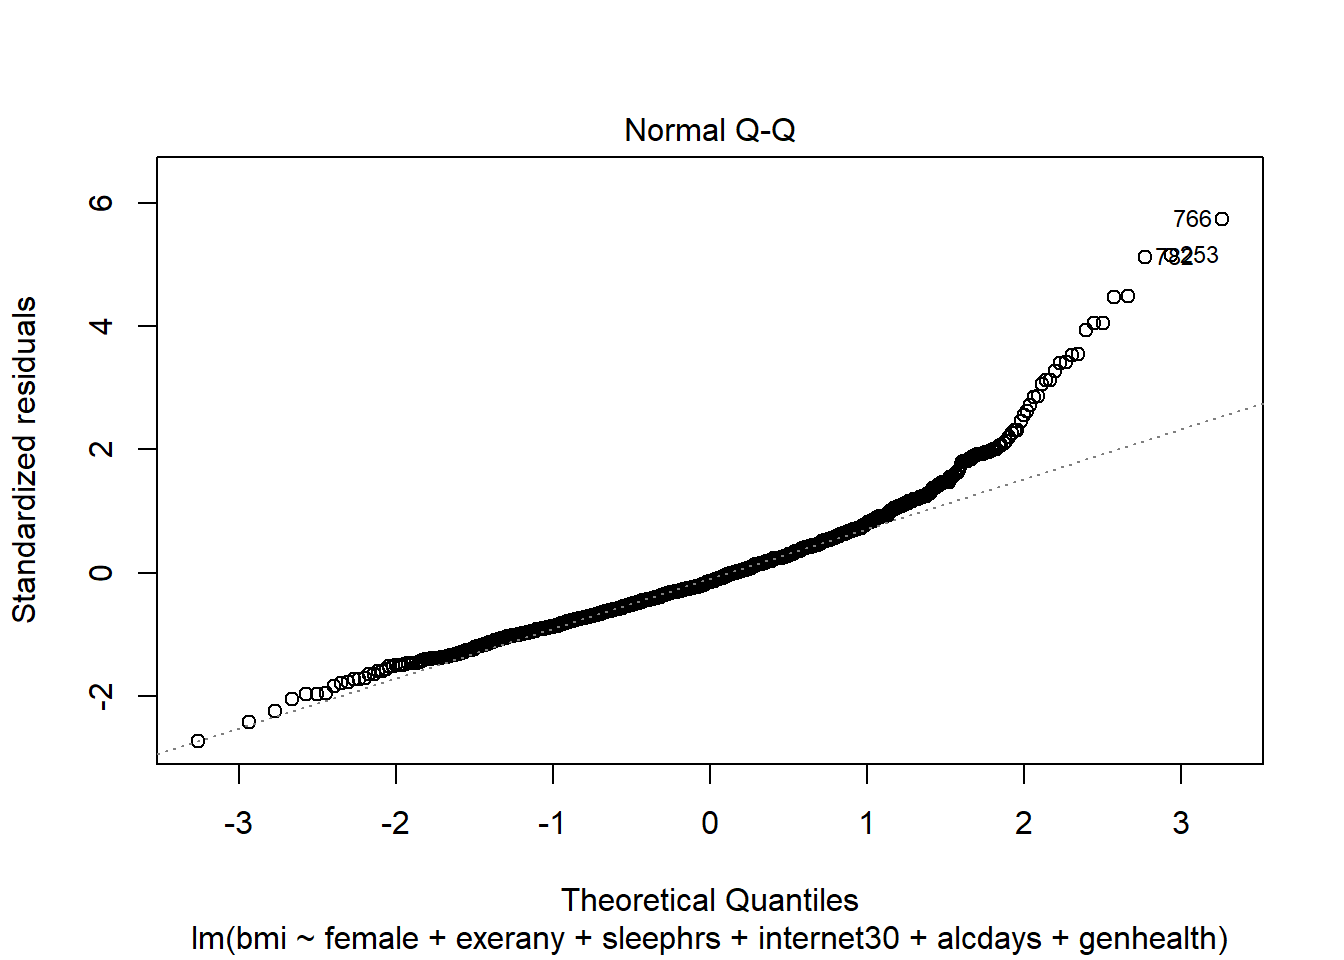
\includegraphics{bookdown-demo_files/figure-latex/unnamed-chunk-11-1.pdf}

\section{m7: What if we added days of work
missed?}\label{m7-what-if-we-added-days-of-work-missed}

\begin{Shaded}
\begin{Highlighting}[]
\NormalTok{c2_m7 <-}\StringTok{ }\KeywordTok{lm}\NormalTok{(bmi }\OperatorTok{~}\StringTok{ }\NormalTok{female }\OperatorTok{+}\StringTok{ }\NormalTok{exerany }\OperatorTok{+}\StringTok{ }\NormalTok{sleephrs }\OperatorTok{+}\StringTok{ }\NormalTok{internet30 }\OperatorTok{+}\StringTok{ }\NormalTok{alcdays }\OperatorTok{+}\StringTok{ }
\StringTok{                }\NormalTok{genhealth }\OperatorTok{+}\StringTok{ }\NormalTok{physhealth }\OperatorTok{+}\StringTok{ }\NormalTok{menthealth,}
         \DataTypeTok{data =}\NormalTok{ smartcle2)}
\KeywordTok{summary}\NormalTok{(c2_m7)}
\end{Highlighting}
\end{Shaded}

\begin{verbatim}

Call:
lm(formula = bmi ~ female + exerany + sleephrs + internet30 + 
    alcdays + genhealth + physhealth + menthealth, data = smartcle2)

Residuals:
    Min      1Q  Median      3Q     Max 
-16.060  -3.804  -0.890   2.794  33.972 

Coefficients:
                    Estimate Std. Error t value Pr(>|t|)    
(Intercept)         25.88208    1.31854  19.629  < 2e-16 ***
female              -0.96435    0.41908  -2.301 0.021616 *  
exerany             -1.43171    0.50635  -2.828 0.004797 ** 
sleephrs            -0.08033    0.13624  -0.590 0.555583    
internet30           2.00267    0.53759   3.725 0.000207 ***
alcdays             -0.07997    0.02528  -3.163 0.001614 ** 
genhealth2_VeryGood  2.09533    0.59238   3.537 0.000425 ***
genhealth3_Good      3.90949    0.60788   6.431 2.07e-10 ***
genhealth4_Fair      4.27152    0.83986   5.086 4.47e-07 ***
genhealth5_Poor      1.26021    1.31556   0.958 0.338361    
physhealth           0.06088    0.03005   2.026 0.043064 *  
menthealth           0.06636    0.03177   2.089 0.037021 *  
---
Signif. codes:  0 '***' 0.001 '**' 0.01 '*' 0.05 '.' 0.1 ' ' 1

Residual standard error: 5.964 on 884 degrees of freedom
Multiple R-squared:  0.1219,    Adjusted R-squared:  0.111 
F-statistic: 11.16 on 11 and 884 DF,  p-value: < 2.2e-16
\end{verbatim}

\begin{enumerate}
\def\labelenumi{\arabic{enumi}.}
\tightlist
\item
  How do the assumptions behind this model look?
\end{enumerate}

\begin{Shaded}
\begin{Highlighting}[]
\KeywordTok{plot}\NormalTok{(c2_m7, }\DataTypeTok{which =} \DecValTok{1}\NormalTok{)}
\end{Highlighting}
\end{Shaded}

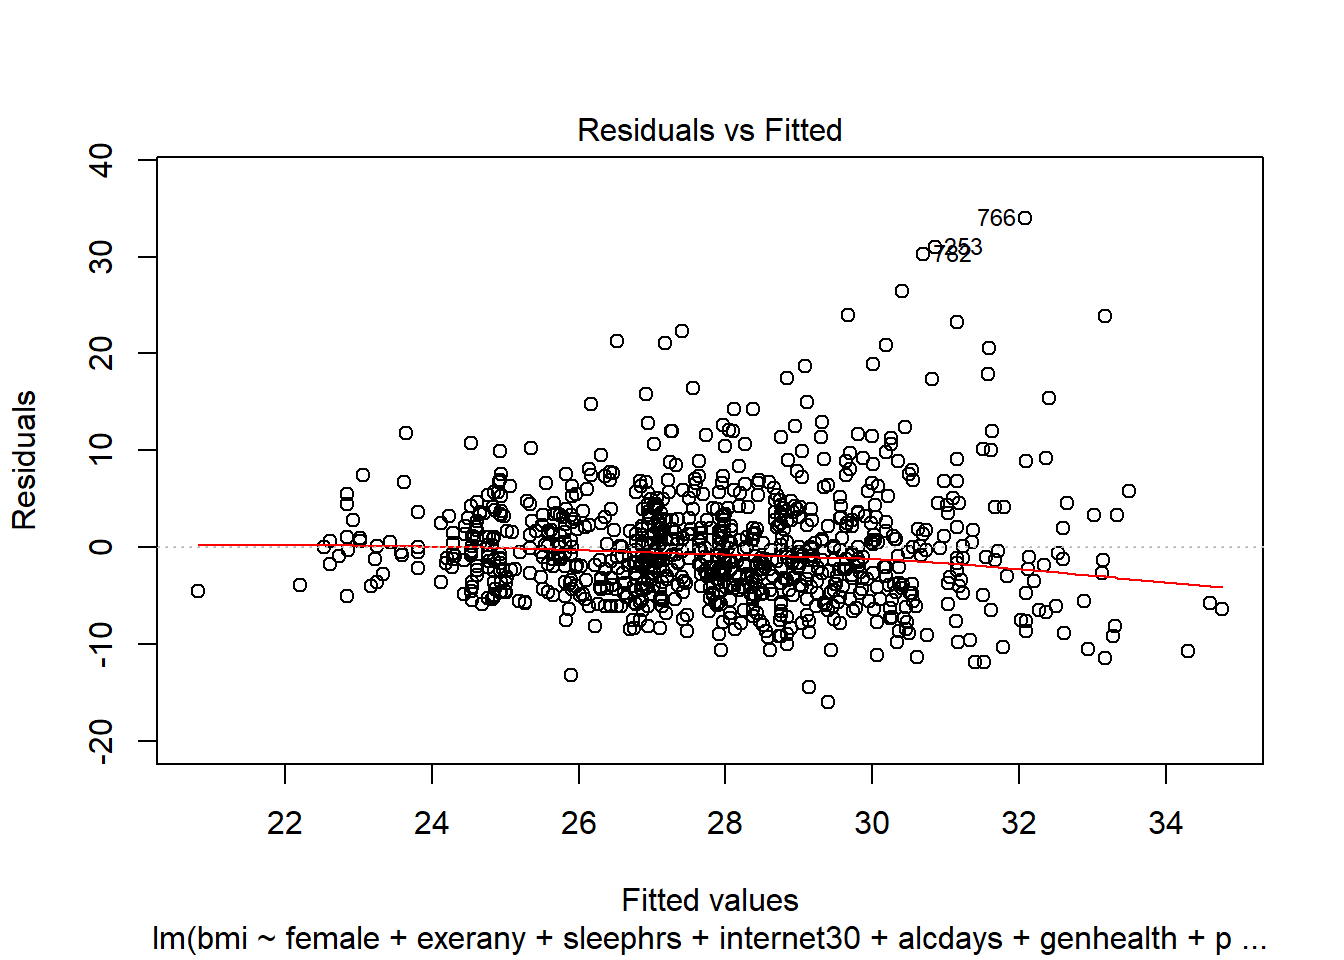
\includegraphics{bookdown-demo_files/figure-latex/unnamed-chunk-13-1.pdf}

\begin{enumerate}
\def\labelenumi{\arabic{enumi}.}
\setcounter{enumi}{1}
\tightlist
\item
  What can we conclude from the plot below?
\end{enumerate}

\begin{Shaded}
\begin{Highlighting}[]
\KeywordTok{plot}\NormalTok{(c2_m7, }\DataTypeTok{which =} \DecValTok{5}\NormalTok{)}
\end{Highlighting}
\end{Shaded}

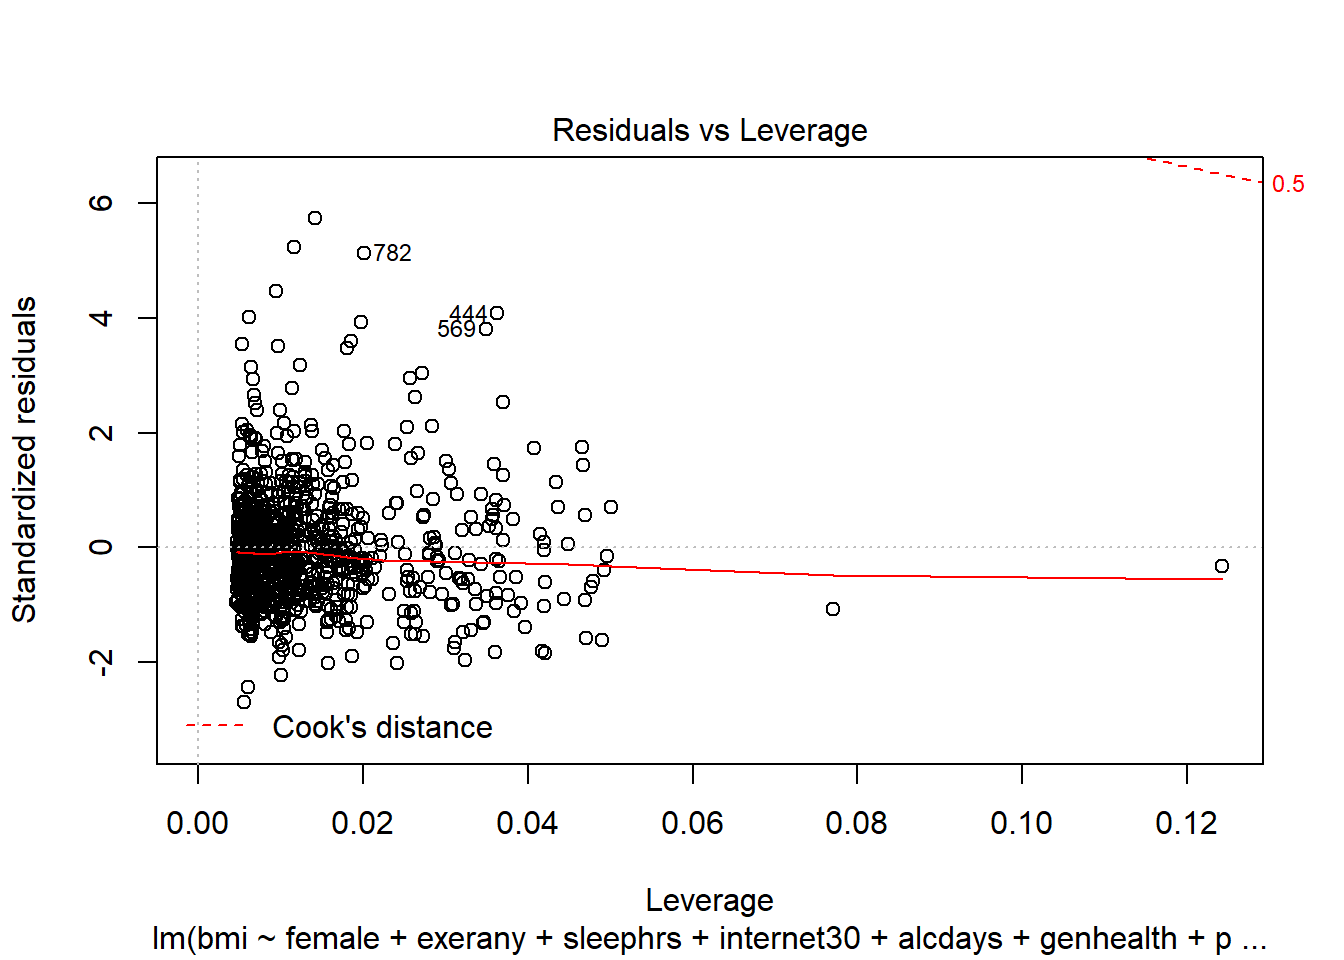
\includegraphics{bookdown-demo_files/figure-latex/unnamed-chunk-14-1.pdf}

\section{How might we validate this
model?}\label{how-might-we-validate-this-model}

Here's some early code for that issue, which is built on some material
by David Robinson at \url{https://rpubs.com/dgrtwo/cv-modelr}

This bit of code performs 10-crossfold separation (splits the data into
10 exclusive partitions and uses each partition for a test vs.~training
split), then maps a modeling step to the training data (which is 10\% of
the full data), and then fits the resulting model on the new data with
augment from the \texttt{broom} package. We've selected the variables so
that the model we'll fit is the \texttt{m2\_c7} model from above.

\begin{Shaded}
\begin{Highlighting}[]
\KeywordTok{set.seed}\NormalTok{(}\DecValTok{4320118}\NormalTok{)}

\NormalTok{models <-}\StringTok{ }\NormalTok{smartcle2 }\OperatorTok
\StringTok{    }\KeywordTok{select}\NormalTok{(bmi, female, exerany, sleephrs, }
\NormalTok{           internet30, alcdays, genhealth) }\OperatorTok
\StringTok{    }\KeywordTok{crossv_kfold}\NormalTok{(}\DataTypeTok{k =} \DecValTok{10}\NormalTok{) }\OperatorTok
\StringTok{    }\KeywordTok{mutate}\NormalTok{(}\DataTypeTok{model =} \KeywordTok{map}\NormalTok{(train, }\OperatorTok{~}\StringTok{ }\KeywordTok{lm}\NormalTok{(bmi }\OperatorTok{~}\StringTok{ }\NormalTok{., }\DataTypeTok{data =}\NormalTok{ .)))}

\NormalTok{predictions <-}\StringTok{ }\NormalTok{models }\OperatorTok
\StringTok{    }\KeywordTok{unnest}\NormalTok{(}\KeywordTok{map2}\NormalTok{(model, test, }\OperatorTok{~}\StringTok{ }\KeywordTok{augment}\NormalTok{(.x, }\DataTypeTok{newdata =}\NormalTok{ .y)))}

\NormalTok{predictions}
\end{Highlighting}
\end{Shaded}

\begin{verbatim}
# A tibble: 896 x 10
   .id     bmi female exerany sleephrs internet30 alcdays genhealth  
   <chr> <dbl>  <int>   <int>    <int>      <int>   <int> <fct>      
 1 01     24.1      0       1        7          1       2 1_Excellent
 2 01     36.4      0       1        8          1       0 4_Fair     
 3 01     32.1      1       0        4          1       5 2_VeryGood 
 4 01     27.3      0       1        8          1       0 1_Excellent
 5 01     28.0      0       1        7          1       4 2_VeryGood 
 6 01     22.5      1       1        7          1       3 2_VeryGood 
 7 01     26.3      0       1        7          1       1 1_Excellent
 8 01     22.4      0       1        8          1       4 1_Excellent
 9 01     19.3      1       0        6          1       0 3_Good     
10 01     24.2      1       0        6          0       0 3_Good     
# ... with 886 more rows, and 2 more variables: .fitted <dbl>, .se.fit
#   <dbl>
\end{verbatim}

The results are a set of predictions (one for each of the original
observations) based on the splits into training and test groups
(remember there are 10 of them, indexed by \texttt{.id}) that describe
the complete set of 896 respondents again.

What this lets us now do is calculate the root Mean Squared Prediction
Error (RMSE) and Mean Absolute Prediction Error (MAE) for this model
(the \texttt{c2\_m7} model) across these observations, and also to
compare that error to a model that simply predicts the mean \texttt{bmi}
across all patients (the \texttt{intercept\ only} model.) In practice,
we could consider two distinct models in doing this work.

\begin{Shaded}
\begin{Highlighting}[]
\NormalTok{predictions }\OperatorTok
\StringTok{    }\KeywordTok{summarize}\NormalTok{(}\DataTypeTok{RMSE_c2_m7 =} \KeywordTok{sqrt}\NormalTok{(}\KeywordTok{mean}\NormalTok{((bmi }\OperatorTok{-}\StringTok{ }\NormalTok{.fitted) }\OperatorTok{^}\DecValTok{2}\NormalTok{)),}
              \DataTypeTok{MAE_c2_m7 =} \KeywordTok{mean}\NormalTok{(}\KeywordTok{abs}\NormalTok{(bmi }\OperatorTok{-}\StringTok{ }\NormalTok{.fitted)),}
              \DataTypeTok{RMSE_interceptonly =} \KeywordTok{sqrt}\NormalTok{(}\KeywordTok{mean}\NormalTok{((bmi }\OperatorTok{-}\StringTok{ }\KeywordTok{mean}\NormalTok{(bmi))}\OperatorTok{^}\DecValTok{2}\NormalTok{)),}
              \DataTypeTok{MAE_interceptonly =} \KeywordTok{mean}\NormalTok{(}\KeywordTok{abs}\NormalTok{(bmi }\OperatorTok{-}\StringTok{ }\KeywordTok{mean}\NormalTok{(bmi))))}
\end{Highlighting}
\end{Shaded}

\begin{verbatim}
# A tibble: 1 x 4
  RMSE_c2_m7 MAE_c2_m7 RMSE_interceptonly MAE_interceptonly
       <dbl>     <dbl>              <dbl>             <dbl>
1       6.03      4.40               6.32              4.59
\end{verbatim}

Another thing we could do with this is to graph the size of the errors
we see in our model.

\begin{Shaded}
\begin{Highlighting}[]
\NormalTok{predictions }\OperatorTok
\StringTok{    }\KeywordTok{mutate}\NormalTok{(}\DataTypeTok{errors =}\NormalTok{ bmi }\OperatorTok{-}\StringTok{ }\NormalTok{.fitted) }\OperatorTok
\StringTok{    }\KeywordTok{ggplot}\NormalTok{(., }\KeywordTok{aes}\NormalTok{(}\DataTypeTok{x =}\NormalTok{ errors)) }\OperatorTok{+}
\StringTok{    }\KeywordTok{geom_histogram}\NormalTok{(}\DataTypeTok{bins =} \DecValTok{30}\NormalTok{, }\DataTypeTok{fill =} \StringTok{"darkviolet"}\NormalTok{, }\DataTypeTok{col =} \StringTok{"yellow"}\NormalTok{) }\OperatorTok{+}\StringTok{ }
\StringTok{    }\KeywordTok{labs}\NormalTok{(}\DataTypeTok{title =} \StringTok{"Cross-Validated Errors in Prediction of BMI"}\NormalTok{,}
         \DataTypeTok{subtitle =} \StringTok{"Using a model (`c2_m7`) including 6 regression inputs"}\NormalTok{,}
         \DataTypeTok{caption =} \StringTok{"SMART BRFSS 2016 data for Cleveland-Elyria MMSA, n = 896"}\NormalTok{,}
         \DataTypeTok{x =} \StringTok{"Error in predicting BMI"}\NormalTok{)}
\end{Highlighting}
\end{Shaded}

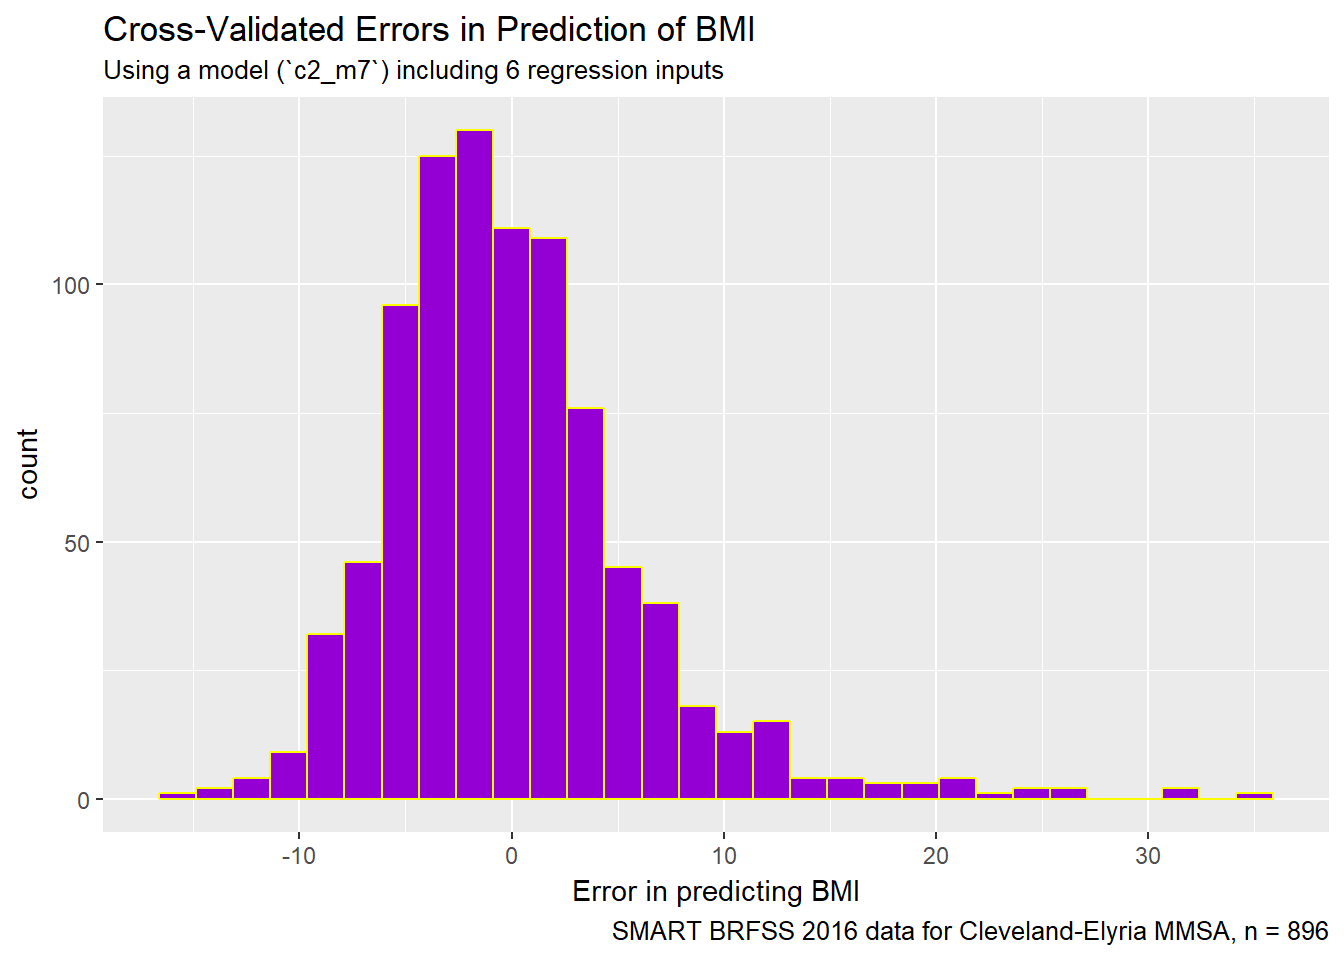
\includegraphics{bookdown-demo_files/figure-latex/unnamed-chunk-17-1.pdf}

\section{Coming Soon to this
Space\ldots{}}\label{coming-soon-to-this-space}

\begin{itemize}
\tightlist
\item
  Would stepwise regression help us build a better model for
  \texttt{bmi}?

  \begin{itemize}
  \tightlist
  \item
    Is there a better approach for variable selection?
  \end{itemize}
\item
  How should we think about potential transformations of these
  predictors?

  \begin{itemize}
  \tightlist
  \item
    What's a Spearman rho-squared plot, and how might it help us decide
    how to spend degrees of freedom on non-linear terms better?
  \end{itemize}
\end{itemize}

\bibliography{text.bib}


\end{document}
